\chapter{Plan Execution and Monitoring}
\label{sec:plan_execution_and_monitoring}

Ghallab et al. point out several types of deliberation functions required for the successful deployment of autonomous artificial agents in diverse environments,
such as \textit{planning}, \textit{acting}, \textit{monitoring}, \textit{goal reasoning}, \textit{reasoning about sensing and information gathering}, and \textit{learning}. \cite{GNT:2016} This chapter deals with arguably the most
fundamental - \textit{planning}, \textit{acting} and \textit{monitoring}. Although, it is not about the plan generation itself, but rather about the handling and execution of given plans.
A key aspect of dealing with some of the potential issues introduced in section \ref{sec:challenges_for_lta} is going to be that the robot will not be able to
complete its missions without preempting the plan execution from time to time. Either due to insufficient battery capacity or other unmanageable conditions such as 
drastic weather changes that force the robot to interrupt its task. As Harris et al. remark: \textquote{\textit{Fixed plans may fail if states encountered during execution do not
sufficiently reflect the assumptions made during plan generation}}. \cite{Harris:2021} Although the overall route may always be the same for the same field, there are certain stopping
conditions that cause the robot to interrupt its active scanning tour and possibly drive back to its base, i.e., the mobile container.
There are generally two relevant perspectives. First, such stops have to be considered at planning time by acknowledging charge stops as crucial part of the plan.
Of course, this is only covering plannable stops such as expected battery consumption and is not able to deal with unplanned situations.
Therefore, a second perspective comes into play, that will be particularly relevant in this work - the execution time.
Just as important as the planning itself is the execution of the generated plan as well as monitoring the execution. Execution monitoring enables a robotic system to
recognize and classify failure situations caused by unexpected internal (robot) or external (environment) states. \cite{Pettersson:2005}
The idea is that the robot executes a given plan and is somehow capable of realizing that it has to interrupt the execution due to some unexpected condition.
In such a case, the robot needs to be able to save the current state of the plan execution and continue precisely with this state after the reason 
for the interruption has been resolved. Consequently, the robot has to be prepared to pause and resume the execution of a given plan, which is far from 
trivial, since the original plan may no longer be applicable for various reasons. This aspect is discussed further in section \ref{sec:plan_interruption_section}.
In this work, \textit{monitoring} is not meant to monitor plan execution in the sense of evaluating
pre- and post-conditions of specific high-level actions and the like, but is to be understood in a more general sense to monitor aspects of the robot system as well as its environment
that have been identified as critical to successful long-term autonomous deployment (cf. sec. \ref{sec:challenges_for_lta}). Essentially, the things that are implicitly part of the plan,
like working sensors and a reasonable battery state of charge. \cite{Ingrand:2017} Based on the challenges identified in section \ref{sec:challenges_for_lta}, this includes the use of
proprioceptive as well exteroceptive sensors and information. As Hawes et al. put it: \textquote{\textit{A key strategy for
delivering long-term robustness is the monitoring of system behavior, from the individual component level up to navigation and task behaviors, as well as the ability to restart
system elements on demand}}. \cite{Hawes:2017} Likewise, Furgale et al. assert that long-term autonomous robots need introspection capabilities to recognize internal problems in
the interest of safety. \cite{Furgale:2015} Ingrand et al. perfectly summarize the view of monitoring in this work: \textquote{\textit{Compares what is predicted regarding the robot
activities to what is observed in the world. It detects and interprets discrepancies, performs diagnosis and triggers recovery actions when needed.}} \cite{Ingrand:2017}
As with planning, monitoring always raises the question of the level of the robot architecture at which it is carried out. The idea of this thesis is essentially to do it at an abstract level
defined by the rough notion of being as universal as possible, to achieve some form of reusability while being applicable and useful in the context under consideration. Obviously,
monitoring also takes place at other levels of abstraction, such as monitoring WiFi signal strength or monitoring within \code{move_base_flex}, which reports errors. There is simply
no fundamental answer to the question of where monitoring should take place. Presumably, one could break it down to the fact that monitoring is necessary at all levels of abstraction,
at least in the sense of error treatment.\newline

\noindent
The potential challenges identified in section \ref{sec:challenges_for_lta}, and their subtypes, are generally classified into two categories in this thesis according to their severity:
Those that cause contingencies and those that lead to catastrophes. The essence of these two categories has already been anticipated by the first two classes of problems in the
concluding remarks of section \ref{sec:challenges_for_lta}. Contingencies refer to cases where the robot is confronted with an unexpected event or problem, but its ability to act is
basically preserved, so that it can try to solve the problem itself, e.g., by returning to base. Catastrophes, on the other hand, refer to cases where the robot is no longer capable of
acting or solving the issue, necessitating human intervention. It is roughly equivalent to the definition of Ross et al. described in \cite{Honig:2018}, where
failures are divided into anticipated errors, exceptional errors, and unrecoverable errors based on the recoverability of the system. The ideas are more based on a high-level planning
perspective, as the first two refer to simple backtracking and replanning, respectively, while the last refers to cases where the plan is no longer feasible and replanning is not an
option. Nevertheless, the first two in combination correspond quite well to the view of contingencies in this thesis - contingencies can be dealt with. Similarly, unrecoverable errors
correspond to catastrophes in this work. They also consider socially recoverable failures where the robot relies on assistance from other operators (humans or other robots), which
is also encountered in this work, namely in the case of the catastrophe situations (cf. sec. \ref{sec:fallback_solution}).\newline

\noindent
Initially, section \ref{sec:plan_generation} introduces the plan generation and format. This is followed by section \ref{sec:execution_monitoring_smach_architecture} on the
architecture of the developed execution monitoring state machine. Subsequently, section \ref{sec:black_box} describes a black box to learn from experience that is already part of
the architecture. Section \ref{sec:plan_interruption_section} explains how the problem of plan interruption and resumption is addressed in this work. Eventually, section
\ref{sec:sim_and_mon_of_lta_challenges} presents the developed monitoring and simulation approaches for the identified challenges, and section \ref{sec:solutions_for_lta_challenges}
concludes the chapter with proposed resolutions.

\section{Plan Generation and Format}
\label{sec:plan_generation}

Long-term autonomous robot operation commonly includes following some sort of plan $\pi$. Planning is the process of selecting and ordering actions that must be performed to
achieve an objective. \cite{GNT:2016} While actions generally refer to processes that change the state of the robot or its environment, they can be considered at different
levels of abstraction. \cite{Ingrand:2017} However, since the actual planning is not part of this work, it is assumed that
plans are provided and usable, e.g., handcrafted by a human operator or generated by a planner from the literature.
For the purpose of parsing a plan $\pi$ and making it retrievable via a service call, a ROS node was developed.
In order for the node to parse the plans, they must be formulated in the following CSV format.
Let $A \coloneqq \{$\code{drive_to(lat, lng, theta)}, \code{return_to_base}, \code{charge}, \code{scan}$\}$ be the set of available actions in the considered scenario
described in section \ref{sec:prototype_scenario}.
Each line in a provided CSV file represents one action $a \in A$ of a plan $\pi$. The actions \code{return_to_base}, \code{charge} and \code{scan} have no parameters,
but \code{drive_to(lat, lng, theta)} needs the additional arguments latitude ($lat$), longitude ($lng$), and orientation ($\theta$) of the target pose. As anticipated in section
\ref{sec:prototype_scenario}, \code{drive_to(lat, lng, theta)} causes the robot to drive to the specified latitude and longitude, and take the specified
orientation. Analogously, \code{return_to_base} directs the robot to move to a user-configurable base position. \code{charge} in the simplified case with the charge patch is simply
a call that charges the battery when the robot is located at the corresponding coordinates. Leaving aside the simplifying assumption of charging at the charge patch presented in
section \ref{sec:prototype_scenario} and considering the realistic case with the container infrastructure (cf. sec. \ref{sec:docking_solution}), there are two other implicit actions
- \code{dock} always follows \code{return_to_base} and lets the robot dock to the inductive charging station inside the container and \code{undock} follows \code{scan} and reverses
the docking procedure. Finally, \code{scan} initiates a scanning operation at the robot's current position, using either the \textit{RIEGL} sensor in practice or the dummy node
(cf. sec. \ref{sec:dummy_scanning_node}) in simulation, which saves a simulated \code{LaserScan}\footnote{\textcolor{link-color}{\url{https://docs.ros.org/en/melodic/api/sensor_msgs/html/msg/LaserScan.html}}} or \code{PointCloud2}\footnote{\textcolor{link-color}{\url{https://docs.ros.org/en/lunar/api/sensor_msgs/html/msg/PointCloud2.html}}} to disk, depending on the configuration.
An example for a simple plan is shown in figure \ref{fig:plan_example}.
When the robot executes this plan, it drives to the four specified locations in sequence and records scans.
Afterwards, it returns to the base and recharges its battery. However, acting requires a lot more than only processing abstract actions provided by a plan (cf. sec.
\ref{sec:execution_monitoring_smach_architecture}). \cite{Ingrand:2017}

\vfill
\pagebreak

\begin{figure}[H]
    \centering
    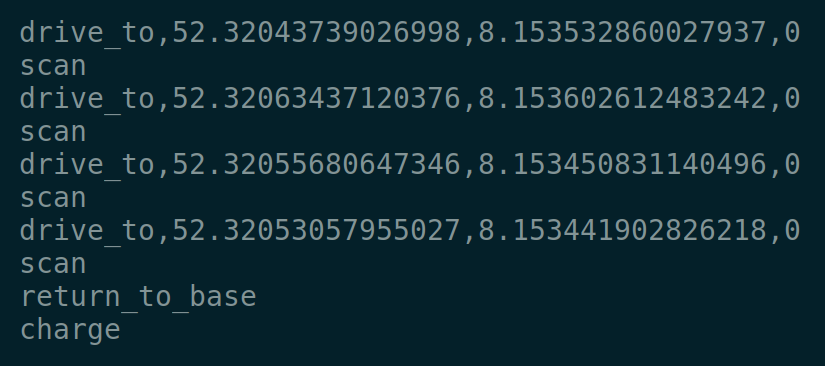
\includegraphics[width=0.5\textwidth]{img/plan_example.png}
    \caption{\textsc{Sample Plan}}
    \label{fig:plan_example}
\end{figure}
\noindent

\section{Execution Monitoring State Machine Architecture}
\label{sec:execution_monitoring_smach_architecture}

Before introducing the developed architecture for plan execution, i.e., \textit{acting} and \textit{monitoring}, it is useful to briefly consider the abstract idea of a general autonomous actor and
classify how these modules fit into the overall construction. Figure \ref{fig:GNT_actor} shows the conceptual view of such an actor based on a visualization by Ghallab et al.
and fig. \ref{fig:MSC_actor} applies this concept to the specific scenario studied in this work.
\begin{figure}[H]
    \centering
    \begin{subfigure}[b]{0.49\textwidth}
        \centering
        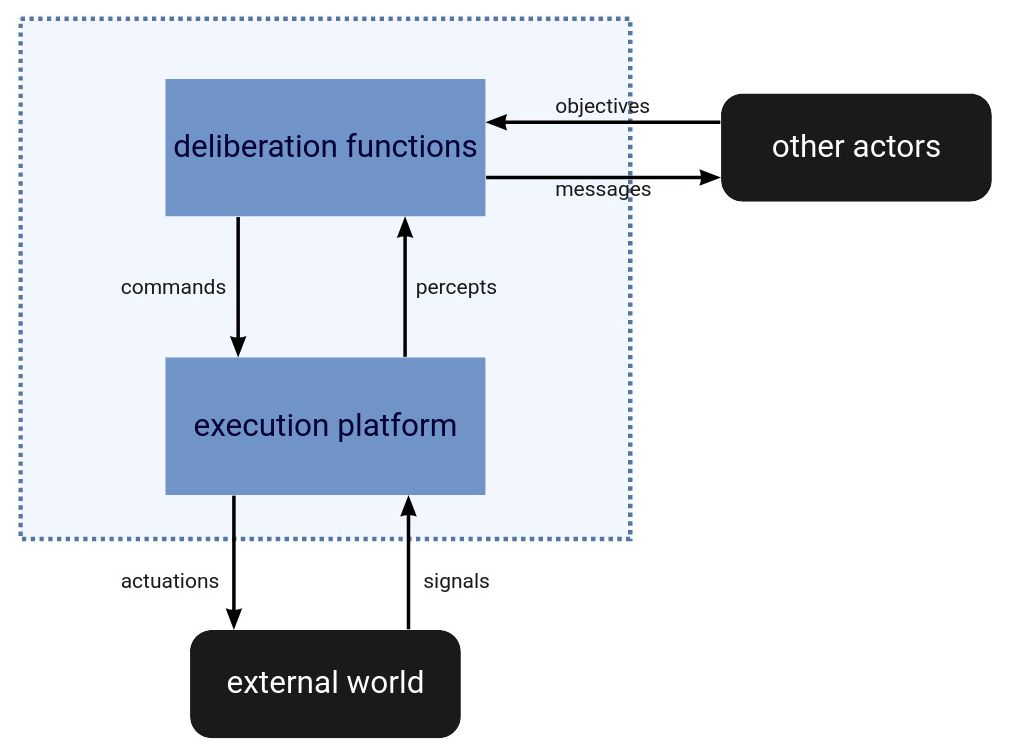
\includegraphics[width=\textwidth]{img/GNT_actor_new.png}
        \caption{\textsc{Actor based on Ghallab et al. \cite{GNT:2016}}}
        \label{fig:GNT_actor}
    \end{subfigure}
    \hfill
    \begin{subfigure}[b]{0.49\textwidth}
        \centering
        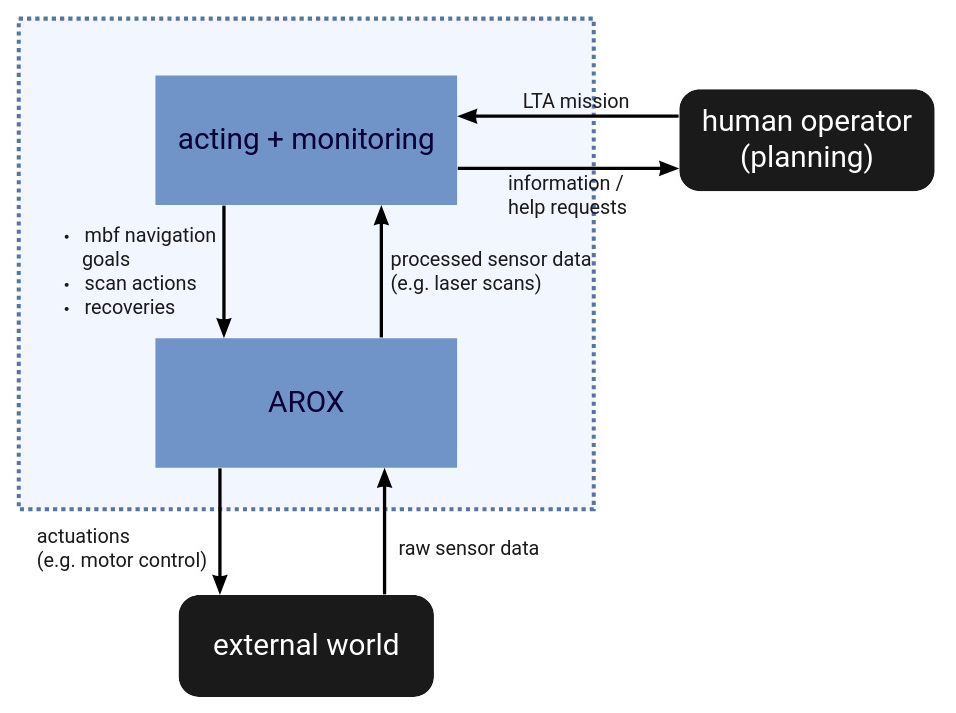
\includegraphics[width=\textwidth]{img/MSC_actor_new.png}
        \caption{\textsc{Applied to the Scenario from Sec. \ref{sec:prototype_scenario}}}
        \label{fig:MSC_actor}
    \end{subfigure}
\caption{\textsc{Abstract Architecture of Autonomous Actors}}
\label{fig:abstract_actor}
\end{figure}
\noindent
As anticipated before and visualized in fig. \ref{fig:abstract_actor}, the deliberation functions studied in this work are \textit{acting} and \textit{monitoring}. Furthermore, \textit{planning} plays a role,
but is only relevant for retrieving and executing plans that are provided by a human operator, i.e., the human operator is essentially the planning component in this scenario.
Moreover, the human operator is the only other actor with whom the robot must interact. The communication between the robot and the operator will be discussed in detail later (cf. sec.
\ref{sec:fallback_solution}), but the general idea is that it is a bidirectional channel that allows the operator to send LTA missions to the robot and, on the
other hand, allows the robot to transmit status information and help requests to the operator. Processed sensor data, mainly in the form of laser scans, is provided to the
acting and monitoring modules by the AROX execution platform presented in section \ref{sec:robotic_system}. Responsible for initiating the actual execution of low-level actions
are also the deliberation functions that are capable of sending commands such as \code{move_base_flex} navigation goals or recovery instructions to the AROX system.
Obviously, the AROX interacts with its environment via its sensors and actuators.\newline
Plan execution, as well as robot operation monitoring, i.e., the \textquote{deliberation functions} module in fig. \ref{fig:abstract_actor}, is modeled as a high-level hierarchically
structured state machine, whose architecture is shown in fig. \ref{fig:high_level_smach}. The capability of a certain degree of fault tolerance is usually not directly integrated
into the control architecture, if considered at all. \cite{Khalastchi:2018} This is different in this thesis.
The architecture is implemented using the SMACH\footnote{ROS-independent Python
library to build hierarchical state machines \cite{smach}} library. The main objectives of monitoring are to detect deviations between what is expected and what is observed
(fault detection), diagnosis of the reasons for such deviations (identification), and provision of recovery options. \cite{Ingrand:2017}
If the behavior of a robotic system is plan-based, i.e., the operations of the robot are determined by some kind of plan, this is very meaningful for monitoring because the current
state of plan execution provides context and thus certain expectations. \cite{Khalastchi:2018} If, for instance, the robot is recording a scan in front of a plant, it may be useful
to start sensor monitoring, i.e., to check whether this operation results in a reasonable-looking scan that is successfully saved to disk.
\begin{figure}[H]
    \centering
    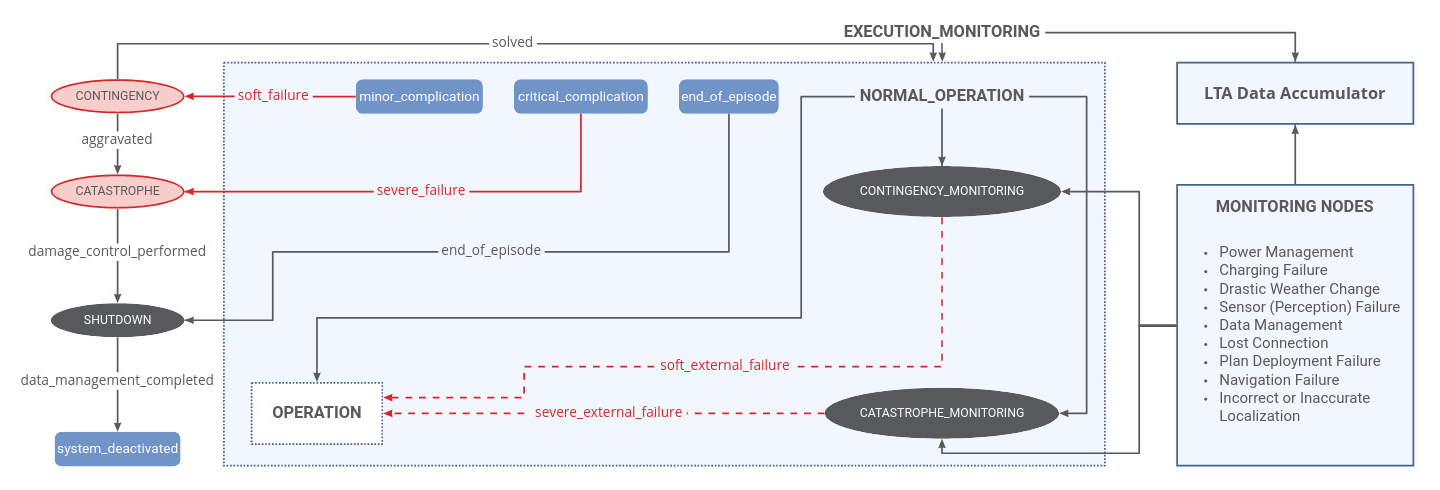
\includegraphics[width=\textwidth]{img/SMACH_high_level.png}
    \caption{\textsc{Architecture of the Hierarchical State Machine (High-Level)}}
    \label{fig:high_level_smach}
\end{figure}
\noindent
As depicted in figure \ref{fig:high_level_smach}, the robot starts in the state \code{NORMAL_OPERATION} in the high-level hierarchical state machine \code{EXECUTION_MONITORING}.
\code{EXECUTION_MONITORING} coordinates the entire robot operation and is composed of the states \code{NORMAL_OPERATION}, \code{CONTINGENCY}, \code{CATASTROPHE}, and \code{SHUTDOWN}.
\code{CONTINGENCY} and \code{CATASTROPHE} essentially refer to type $(1)$ and type $(2)$ in the classification in fig. \ref{fig:problem_types}, respectively.
\code{NORMAL_OPERATION} is represented by an embedded state machine named \code{OPERATION}, visualized in figure \ref{fig:low_level_smach}, as well as the two
parallel running execution monitoring states (cf. ROS \code{MonitorState}\footnote{\textcolor{link-color}{\url{https://wiki.ros.org/smach/Tutorials/MonitorState}}}) \code{CONTINGENCY_MONITORING} and \code{CATASTROPHE_MONITORING}, 
implemented as a concurrence container (cf. SMACH \code{Concurrence}\footnote{\textcolor{link-color}{\url{https://wiki.ros.org/smach/Tutorials/Concurrence\%20container}}}).
These parallel running states are used to monitor the robot's operation and to interrupt it when a problematic situation requiring special treatment is detected
(indicated by the dashed arrows in figure \ref{fig:high_level_smach}).
When this case occurs, based on how severe the problem is, the respective procedure will interrupt \code{OPERATION} and provide for the outcome \code{critical_complication} or
\code{minor_complication}, which will then result in a state transition to the appropriate states in which the issue will be addressed. There is quite a bit behind
\code{CONTINGENCY}, namely the handling of the problem based on the problem type that is communicated along with the message of the interruption.
If \code{CONTINGENCY} is able to solve the issue, \code{NORMAL_OPERATION} will resume (cf. \textquote{solved} arrow). In case of \code{critical_complication} or if the robot is not able to
solve the problem (cf. \textquote{aggravated} arrow), it ends up in the \code{CATASTROPHE} state, the human operator is notified, a backup is made if necessary, etc., and then the robot shuts down.
The interrupts of \code{OPERATION} are initiated by the monitoring nodes, which are shown on the right in fig. \ref{fig:high_level_smach}, and which detect problems as universally
as possible for each identified problem category.
Although a monitoring solution could in principle also be implemented sequentially, it seems more natural to choose a parallel approach, since a sequential option
would have the disadvantage that no monitoring takes place while a task / algorithm is being executed, but only afterwards.
It is desirable to be able to intervene at any time during the execution of a task when a monitoring procedure running in parallel is triggered and causes a change of state.\newline

\noindent
During the state \code{OPERATION}, i.e., in the nested state machine visualized in figure \ref{fig:low_level_smach}, the robot can be either in the state \code{IDLE}, 
in which it is waiting for a plan, or in \code{EXECUTE_PLAN}, in which it is executing a given plan $\pi$. The embedded state machine \code{OPERATION} has 
four possible outcomes - \code{end_of_episode}, \code{minor_complication}, \code{critical_complication}, and \code{preempted}. 
It starts in the \code{IDLE} state and remains there as long as no plan is provided via a ROS service.
There are two common options for the robot to leave the state. The first is via a message on a ROS topic indicating that the end of the current long-term episode
has been reached, resulting in an overall outcome of \code{end_of_episode} for \code{NORMAL_OPERATION} followed by \code{SHUTDOWN} (cf. fig. \ref{fig:high_level_smach}). The second is to receive a plan $\pi$ that results in a state
transition to \code{EXECUTE_PLAN}. Additionally, the external parallel running monitoring states \code{CONTINGENCY_MONITORING} and \code{CATASTROPHE_MONITORING}
are capable of interrupting the \code{IDLE} state at any time (cf. state preemption\footnote{\textcolor{link-color}{\url{https://wiki.ros.org/smach/Tutorials/State\%20Preemption\%20Implementation}}}) due to external problems leading to the outcome \code{preempted}.
In \code{EXECUTE_PLAN}, there are five possible outcomes, two of which result in state transitions and three of which cause \code{OPERATION} to return to the parent state machine.
The first possible outcome is \code{action_completed}, which indicates that an action $a \in \pi$  was completed successfully and causes the same state (\code{EXECUTE_PLAN}) to be
executed again with the reduced plan $\pi \coloneqq \pi \backslash \{a\}$, i.e., the rest of the plan is executed. The next possible outcome is \code{plan_completed}, which means that the entire
plan $\pi$ has been successfully processed, i.e., $\pi = \emptyset$, and causes a transition back to the \code{IDLE} state.
These were the possible outcomes that cause a state transition. Now there are the three remaining outcomes that cause a return to the parent state machine. 
First, \code{soft_failure}, which means that something went wrong, e.g., an action $a \in \pi$ was not performed successfully, but the robot should be able to handle the problem. 
Second, there is the potential outcome \code{severe_failure}, which represents situations where the robot is unable to solve the problem itself.
Finally, the last potential outcome is again \code{preempted} based on some external issue indicated by \code{CONTINGENCY_MONITORING} or \code{CATASTROPHE_MONITORING} and
detected by one of the monitoring nodes.
In summary, there are two types of problems, low-level problems that are detected directly at this level, e.g., by simple error treatment, which then lead to an interruption based
on the severity of the issue, in this case \code{soft_failure} or \code{severe_failure}, which is then passed up to the high-level SMACH and handled accordingly.
The other, much more common case is that a problem is detected by the monitoring nodes (cf. \code{external_problem}) with the consequence that execution is simply interrupted here
and the problem is solved superordinately. Then \code{OPERATION} is restarted.
\begin{figure}[H]
    \centering
    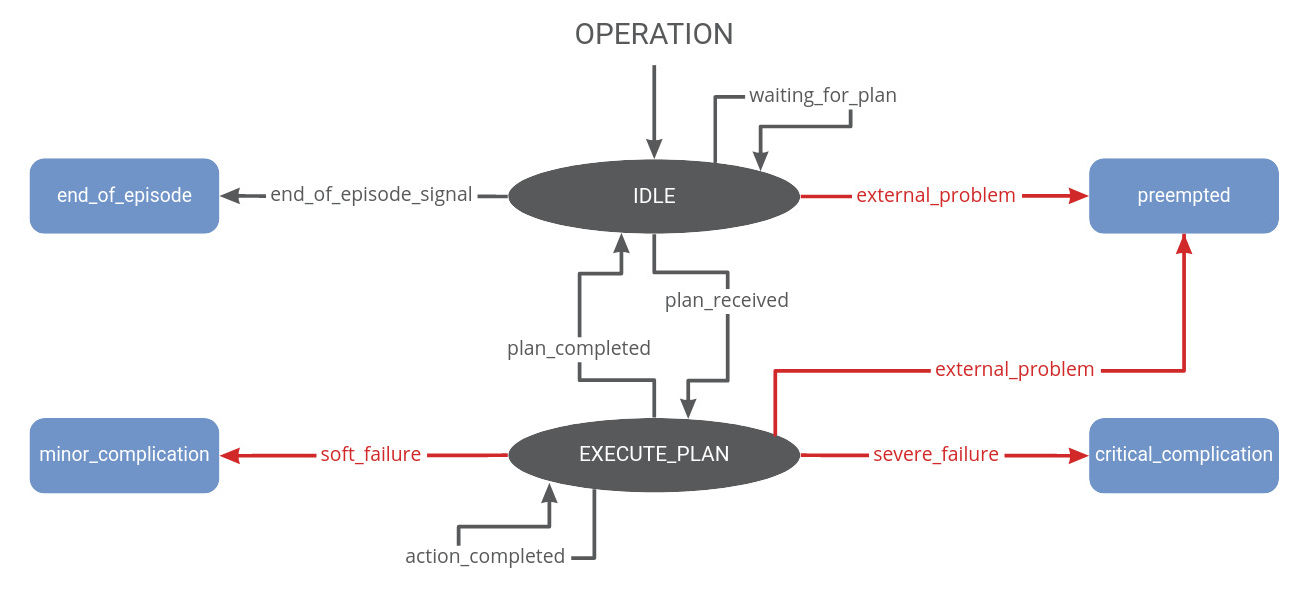
\includegraphics[width=0.8\textwidth]{img/SMACH_low_level.png}
    \caption{\textsc{Architecture of the Embedded State Machine (Low-Level)}}
    \label{fig:low_level_smach}
\end{figure}
\noindent
Now that the control flow of \code{NORMAL_OPERATION} and, in particular, \code{OPERATION} has been clarified, we return to the parent state machine shown 
in figure \ref{fig:high_level_smach}.
As mentioned, when \code{NORMAL_OPERATION} returns \code{end_of_episode}, the parent state machine transitions to the \code{SHUTDOWN} state and the 
robot's work for that long-term episode is complete, which means that the robot performs data management and then the system is deactivated.
Essentially, in a long-term episode in the considered scenario, the robot should stay in \code{NORMAL_OPERATION} as 
long as the episode is running or an error / problem has occurred, either an error that it is able to deal with itself or even a more severe issue that requires the 
intervention of a human operator. Accordingly, if \code{NORMAL_OPERATION}, i.e., the embedded state machine together with the parallel running monitoring states has the outcome 
\code{minor_complication}, the robot enters the state \code{CONTINGENCY}, which means that it has detected a soft failure, e.g., a sensor failure, but its ability to act
is preserved, it is for example able to drive back to the base in safety mode or repeat the scan attempt. However, if \code{NORMAL_OPERATION} returns \code{critical_complication}, there is a severe 
failure that is unsolvable for the robot, perhaps even for the operator, and the robot transitions to \code{CATASTROPHE}. If it is still possible, the robot saves the current 
state of the plan execution, sends an emergency signal, e.g., communicates the problem to the operator, and shuts down, i.e., transitions to \code{SHUTDOWN}.
There are, of course, situations in which the robot can no longer do anything, such as when the battery is completely discharged.
In principle, such cases also fall under the category of catastrophe, but since monitoring then no longer works, there is nothing left to do there.\newline
To be clear, \code{NORMAL_OPERATION} can manage problems in two ways.
First, a problem may occur during plan execution in the child state machine, in such a case \code{OPERATION} returns \code{critical_complication} or 
\code{minor_complication} to the parent state machine based on the problem severity and a corresponding state transition takes place.
In addition, there are the described parallel monitoring states, which are responsible for issues that are not directly related to plan execution, but are of a more general nature.
If these detect an issue, they are able to interrupt \code{OPERATION} and also return \code{critical_complication} or \code{minor_complication} to the parent state machine
\code{EXECUTION_MONITORING}. It is trivial to interrupt \code{OPERATION} when no task is currently being executed, i.e., no scan is being recorded and no navigation target 
is being approached. However, it is obvious that potential problems do not wait for the completion of such tasks, but can also occur during the execution of an action $a \in \pi$.
Therefore, the \code{drive_to(lat, lng, theta)} and \code{scan} actions are implemented as a ROS \code{SimpleActionClient}\footnote{\textcolor{link-color}{\url{http://wiki.ros.org/actionlib}}} that can be interrupted at any time
by calling the \code{cancel_all_goals()} method, which immediately interrupts all running goals. It is quite important that the robot is able to preempt the plan 
execution at all times, e.g., does not continue to drive to its goal, but should instantly stop the \code{move_base_flex} goal execution and start following the
recovery instructions.\newline
The general difference between the \code{CONTINGENCY} and \code{CATASTROPHE} states is the robot's ability to act. 
In a catastrophe case, it is no longer really capable of acting in the sense of driving back to its base, managing the problem itself, etc. 
An example for a catastrophic case would be that the robot falls over. It is then unable to recover, but it is of course still able to communicate the problem
and save the state, in full possession of its ``mental'' powers, so to speak. Whereas a lightning strike, as an extreme example, could cause the robot to have a 
complete breakdown and nothing to work at all. The boundaries there are not quite sharp, there are many edge cases.
The following somewhat more mundane example, considering the robot's battery, will illustrate the concepts.
In \code{NORMAL_OPERATION}, the battery does not discharge precisely according to the plan. There may be some fluctuations due to temperature, for example.
The power management monitoring node would initiate a transition to the state \code{CONTINGENCY} when it detects that the battery is already too low to complete the plan until the
next charge stop, but the robot is still able to recover, i.e., drive back to its base, recharge, and continue the plan execution. However, it would proceed to \code{CATASTROPHE} if it
detects that the battery is so low that it can already tell that it is not possible to reach the base and recharge. The robot is then still able to communicate the problem and save the
state, but it is definitely not able to recover. This leads to a message to \code{CATASTROPHE_MONITORING}, then to an external failure, which interrupts \code{OPERATION} with a
\code{critical_complication} and causes the high-level state machine to transition to \code{CATASTROPHE}. The problem is communicated and the robot shuts down. The extreme case,
where nothing can be done, would be that the battery suddenly just breaks. Finally, there is also the case that first a \code{CONTINGENCY} is launched as the problem still seems to be
solvable based on current estimations and then it turns out that it in fact is not. For instance, when the discharge rate is furthermore increased. In such a case, it turns out during
the solution that it does not work anymore, i.e., the assumption was wrong, it is no longer solvable, then it comes to the \textquote{aggravated} case, i.e., the problem worsens and then
becomes a \code{CATASTROPHE}. Additionally shown in fig. \ref{fig:high_level_smach} is the data accumulator that logs all relevant information from the execution and monitoring nodes.
On the one hand for debugging purposes, but also to be able to learn from it later on, which will be discussed in section \ref{sec:black_box}.

\section{Black Box to Learn from Experience}
\label{sec:black_box}

From a software engineering perspective, it makes sense to create an interface for machine learning or general analysis in the architecture, even if it is not yet explicitly used.
This interface is intended for a concrete configuration, e.g., the AROX system with its sensors (cf. section \ref{sec:robotic_system}), the rationale being to learn from experience. The robot operates in an environment for an
extended period of time. Therefore, it is very valuable to collect data about the robot, its interaction with the environment, faults, etc. through extensive logging, with special
emphasis on fault context. Whenever something goes wrong, it is interesting to learn the reason for this problem. For a specific sensor setup, one could use learning techniques or
statistical methods in general to infer that a particular effect occurs experientially. For instance, experience might show that a particular sensor failure occurs repeatedly when
driving for more than $4$ hours at a temperature above $32$\textdegree{}C. A further example could be that the robot always has a failure after passing a certain waypoint.
To determine this, it would be necessary to always log the current location of the robot along with a problematic situation. This list could be arbitrarily extended.
In general, the objective is to avoid certain behaviors that have frequently led to failures in the past. Information about such effects can only be
obtained through runtime experience, which shows how relevant such information are and how crucial it is to collect them. So gathering information should go along with long-term
operation.\newline

\noindent
The actual learning of such effects is beyond the scope of this thesis. Yet, the creation of an appropriate interface in the architecture and the collection of information
are part of the developed framework. The idea of gathering information and learning from it is natural, because that is essentially what a human operator would do as well, gaining
experience and improving over time. Essentially, in a problematic situation, it is a matter of logging what the associated relevant circumstances are. Of course, this would just be
the output of the system and the input to some sort of learning or analysis software. Nonetheless, if some regularities have been learned or identified from the logged data, they can
be exploited and it should be possible to feed that information back to the system, i.e., the path in the other direction. Unfortunately, since this is usually information of the type
\textit{in the event of $X$, do $Y$}, it is not trivial to feed it back automatically and actually apply it in a meaningful way. It would be possible to report back messages that
indicate problems based on learned regularities, but it is not as simple to create a way to automatically generate an appropriate response from the robot to avoid the problem. There
can be an arbitrary number of possible actions that are required, and the only truly viable solution is to provide a general and easily extensible framework so that learned
regularities can be implemented as advanced monitoring and resolution methods. Now, one could argue that such a feedback option would still be valuable for the learned messages that
indicate issues. However, this does not help significantly, as these messages have already been logged in erroneous situations, which have thus inevitably already been detected by
the existing monitoring solutions. The broad idea of learning from experience in long-term autonomous operation is not new, of course, and some examples have already been given in the
literature review in section \ref{sec:literature_review}. Hawes et al. \cite{Hawes:2017} also emphasize the usefulness of the information gathered in long-term autonomous operation for both learning and troubleshooting
purposes. For information gathering, they use \code{mongodb_store}\footnote{\textcolor{link-color}{\url{https://wiki.ros.org/mongodb\_store}}}, a ROS tool for storing data from a ROS system (messages,
configurations, etc.) in a \textit{MongoDB} instance, i.e., a document-oriented database. To achieve systematic and reusable logging and general data acquisition, this tool is also
used in this thesis. For this purpose, a \code{data_accumulator} node was written to capture the relevant data during LTA missions and store it in the database.\newline

\noindent
Initially, a
\code{MessageStoreProxy} object is created to enable updating and maintenance of the \textit{MongoDB} database. Various logging categories are defined to semantically group the
collected data. Each component of the monitoring framework, i.e., each node, can initiate logging to the database under a specific category based on ROS topics provided by the
\code{data_accumulator}. To store an entry under a category or name, the \code{insert_named("name", entry)} method of the \code{MessageStoreProxy} is used. It is obviously relevant
to log contingency and catastrophe situations, which is why \code{/contingency_preemption} and \code{/catastrophe_preemption}, the topics to initiate interruptions via the parallel
monitoring nodes introduced in section \ref{sec:execution_monitoring_smach_architecture}, lead directly to a database entry under the categories \code{contingency} and
\code{catastrophe}, respectively. The content of this entry is in each case the message describing the problem that occurred. Whenever a contingency or
catastrophe situation is logged, the node triggers a method \code{log_failure_circumstances()} because, as mentioned earlier, the particular circumstances of a problematic
situation, i.e., the potential factors leading to the problem, can be very revealing. For the moment, the specific additional contextual information comprises, in addition to the
information logged anyway, the position of the robot in longitude and latitude obtained from \code{/fix} (cf. sec. \ref{sec:sim_and_mon_gnss_connection_problems}), as well as the
number of tasks completed, the current operating time, the charge level and the current charge cycle. This
list can be extended in the future as needed. All this information is stored summarized in a JSON dump under the category \code{failure_circumstances}. Numerous insightful but less
critical information about the robot and its environment is logged under the category \code{robot_info}, received as messages on a topic with the same name. When conducting
experiments in a simulated environment, it is also vital to know precisely when error situations have been simulated. Therefore, all nodes simulating problem conditions can report
under the topic \code{/sim_info} once they do so, at which time the messages are stored in the database. The \code{/action_info} topic is responsible for logging the also very
relevant information about the currently executed action. Moreover, there are \code{/operator_communication} and \code{/resolution} that store all exchanged messages between the
operator and the robot, as well as all executed resolution methods. It is furthermore important to keep track of missions,
which is why new messages via \code{/arox/ongoing_operation} are also logged. Finally, for debugging purposes, there is a \code{/show_db_entries} topic that allows to list
all database entries for the current LTA mission or the entries under a particular category specified by the string message published to the topic.\newline

\noindent
The path for the
database can be configured in the launch file. Once a \textit{MongoDB} server is running with the generated database, i.e., \code{mongod --dbpath ROS_db --storageEngine=wiredTiger},
a \textit{MongoDB} client can connect and examine the logged data. It can be visualized and queried in JSON, for example, as shown in fig. \ref{fig:database_entries}.
This shows, for instance, a contingency due to a failed docking attempt. This is immediately followed by the explicit error conditions, e.g., state of charge, tasks completed, charge
cycle, position and operating time. Besides, many aspects that are logged at the same time under \code{robot_info} are not displayed here. Subsequently, the resolution follows, the
charging failure resolver is started together with the information describing the problem.
\begin{figure}[H]
    \centering
    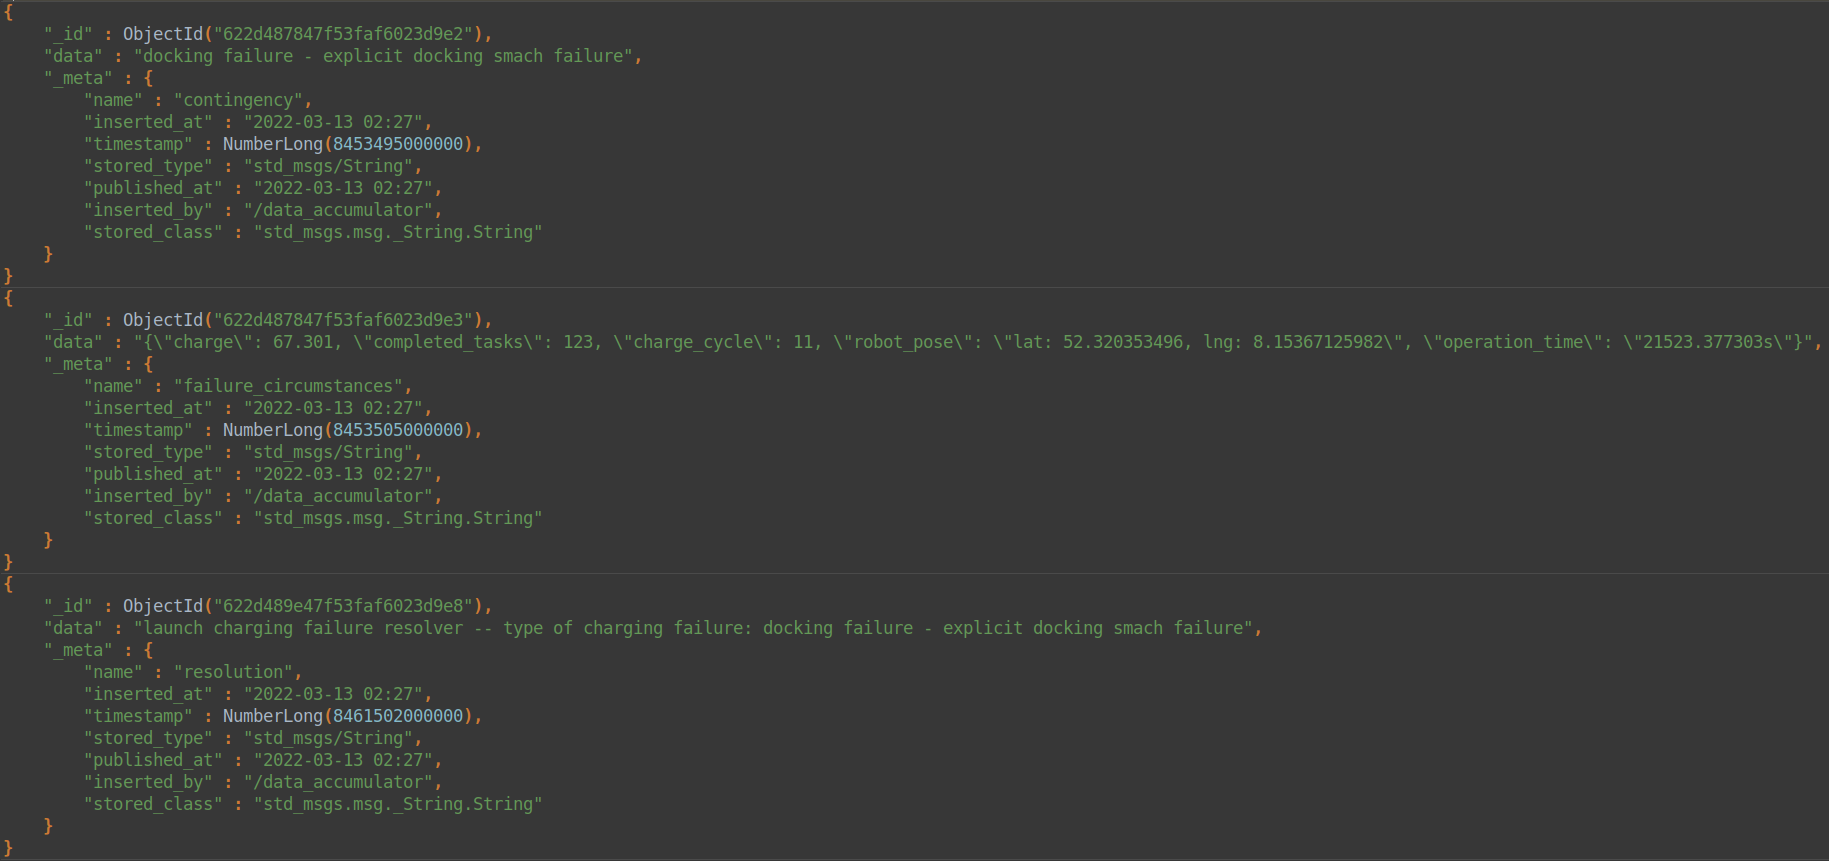
\includegraphics[width=\textwidth]{img/database_entries.png}
    \caption{\textsc{Database Entries Shown in} \textit{MongoDB} \textsc{Client}}
    \label{fig:database_entries}
\end{figure}

\section{Interruption and Resumption of Normal Operation}
\label{sec:plan_interruption_section}

\textquote{\textit{Plans must be executed according to some strategy. This must account for action failure, plan failure due to ignorance or change in a dynamic environment,
and changing mission requirements.}}
\cite{Cashmore:2015}
In order to handle unexpected problematic situations, the robot must be able to stop and resume its normal operation in general
and plan execution in particular, i.e., to save the current state of the plan execution and resume exactly that state after the reason
for the interruption has been resolved. The idea is that whenever the monitoring nodes introduced in section \ref{sec:execution_monitoring_smach_architecture} or the plan execution
itself detect a problem, \code{CONTINGENCY_MONITORING} or \code{CATASTROPHE_MONITORING} should trigger such an interruption.
As seen in section \ref{sec:execution_monitoring_smach_architecture}, there are two states in \code{OPERATION} that the robot can be in during a long-term episode without any problems
- \code{IDLE} or \code{EXECUTE_PLAN}. In the \code{IDLE} state, where it waits for the plan generator described in section \ref{sec:plan_generation} to provide a plan $\pi$,
it is straightforward, the normal operation is interrupted, the high-level state machine transitions to \code{CONTINGENCY} or \code{CATASTROPHE} depending
on the severity of the problem, and then, i.e., when the minor problem is resolved, it transitions back to \code{IDLE} or shuts down in the case of \code{CATASTROPHE}.\newline
The more interesting case, of course, is such an interruption of the normal operation when the robot is in the low-level state \code{EXECUTE_PLAN}.
In this case, a plan execution must be interrupted.
During the \code{EXECUTE_PLAN} state, the currently executed plan $\pi$ is always stored in the \code{userdata} field of the state.
SMACH states always provide a so-called \code{userdata} field, which is essentially the input and output data of a SMACH state.
Initially, when \code{IDLE} receives a plan $\pi$ from the plan generator, it passes it as \code{userdata} to the \code{EXECUTE_PLAN} state. Then, whenever \code{EXECUTE_PLAN}
successfully completes an action $a \in \pi$, the reduced plan, i.e., $\pi \coloneqq \pi \backslash \{a\}$, is passed to the next iteration of the same state.
Therefore, based on this architecture, the current state of the plan execution is always stored in the \code{userdata} of the SMACH. To comply with this fact, a certain situation
must be handled. If a plan execution is interrupted during the execution of an action $a \in \pi$, the action $a$ is already removed from the plan $\pi$, i.e., the \code{userdata},
by the latest \textit{pop} operation, and since the execution of $a$ must be repeated when the normal operation resumes, $a$ must be reattached to $\pi$ before transitioning
to \code{CONTINGENCY} or \code{CATASTROPHE}. Thus, $\pi \coloneqq a.\pi$ (concatenation of action and plan). Yet, there is a special case: If an interruption occurs during a \code{scan}
action and the interruption involves leaving the scan position, the robot must return to that position before repeating the scan, which means that the last \code{drive_to} action
before the scan must also be repeated. Of course, when the robot transitions back to \code{NORMAL_OPERATION} after solving a contingency, it starts again in \code{IDLE}, which is why \code{IDLE}
always looks for existing unfinished plans $\pi$ in the \code{userdata} first. If there is one, i.e., $\pi \in$ \code{userdata.input_plan}, $\pi \neq \emptyset$, it does not prompt the
plan generator for a new plan, but continues the previously preempted and only partially completed plan $\pi$.
The catastrophe case works analogously to the \code{IDLE} state.\newline

\noindent
Of course, it is not necessarily always feasible to simply execute the rest of the plan afterwards, since the planned charge stops may no longer be sufficient. However, if the
interruption of the plan involves returning to the base and seeking shelter, this is not a problem, since such a recovery can always be accompanied by recharging, so that the
battery is fully charged when the robot resumes its operation. In such a case, it might even be feasible to remove some of the next planned charge stops. If a charge stop is one
of the actions immediately following, this simple plan modification is performed. Nevertheless, there are cases in which the robot does not return to the base and has to consume
unplanned resources, so that the a priori planned charge stops are rendered insufficient. This problem, though, is addressed by the integrated battery monitoring module described
in section \ref{sec:battery_monitoring}, which detects this and initiates a return to base. In conclusion, the continuation of plan execution works either way.

\vfill
\pagebreak

\section{Simulation and Monitoring of LTA Challenges}
\label{sec:sim_and_mon_of_lta_challenges}

Now that the overall architecture of the execution monitoring state machine has been described (cf. section \ref{sec:execution_monitoring_smach_architecture}) and it is clear how to
interrupt the operation, we can turn to the actual monitoring methods for the potential hinderances for long-term autonomous systems introduced in section \ref{sec:challenges_for_lta}.
The idea is to implement a specific monitoring procedure for each of the selected LTA challenge categories that runs in parallel to the high-level state machine. Whenever such a
procedure is triggered, i.e., a specific issue
is recognized, the problem gets reported via the \code{MonitorState}, causing a transition to \code{CONTINGENCY} or \code{CATASTROPHE} based on the severity of the problem.
Depending on the nature of the issue, the information about the required solution method is conveyed via the message published to the topic of the \code{MonitorState}.
Thus, the long-term goal is to have a resolver node for each of the potential failures, which is executed in \code{CONTINGENCY} or \code{CATASTROPHE} depending on the
failure case at hand. While in the case of contingencies these nodes actually refer to problem solving, in catastrophe cases they are more for damage control, since catastrophes
by definition cannot be solved by the robot itself.
It is useful to distinguish between internal and external exceptional situations that require special treatment, i.e., issues concerning the robotic
system itself or the environmental conditions. \cite{Hawes:2017}
The entire process is essentially the same for all potential LTA challenges - fault simulation, monitoring, and subsequent remediation.
An important aspect is that the focus is not on the reasons for problems occurring, but only on detection. There can be arbitrarily many reasons why certain aspects of the system
are not functioning properly, and it is unrealistic to contemplate them all. The critical point is to recognize that there is an issue, not why.
If the robot had the chance to recognize a causality, it could specifically pursue it, but this is typically not the case.
Accordingly, the approach is always to think about how to determine that something is dysfunctional, which greatly reduces the number of possibilities.
For instance, the number of ways a laser scanner can malfunction is much smaller than the number of reasons for malfunction.\newline

\noindent
Initially, it will be demonstrated that in the
prototypical scenario, the mission can no longer be completed successfully if these errors occur (cf. section \ref{sec:experiments}). After launching the monitoring nodes, the
problems should be detected and either resolved by the robot or reported to the operator so that the mission can continue. All of the failure simulations are implemented in a way that
allows them to be triggered by publishing to a certain topic in order to enable automation of these failure cases in subsequent experiments (cf. section \ref{sec:experiments}).
In the following, the simulation of the selected LTA problems is presented along with the monitoring solutions developed for each.

\subsection{Power Management}
\label{sec:sim_and_mon_power_management}

Power management issues are addressed based on the integrated battery watchdog module described in section \ref{sec:battery_monitoring}, which monitors the state of the battery
and acts as a fail-safe. The integrated watchdog module constantly publishes one of three states on the topic \code{/watchdog}. \code{"NORM"} indicates that the energy consumption is
as expected and no problem has been detected. In contrast, \code{"CONT"} and \code{"CATO"} represent situations in which the a priori planned charge stops are no longer feasible. In the
event of a contingency, i.e., \code{"CONT"}, an immediate return to the base station is required in order to still be able to reach it. Even more severe, in a catastrophe situation, i.e.,
\code{"CATO"}, it is no longer possible to reach the base station due to the battery charge level. The monitoring node simply subscribes to the \code{/watchdog} topic and initiates
appropriate responses based on the signals sent by the battery watchdog module. In case of a \code{"CONT"} message, \code{/contingency_preemption} is used to initiate a contingency
and communicate the specific reason. Likewise, in case of \code{"CATO"}, a catastrophe is triggered with \code{/catastrophe_preemption}. The node distinguishes between catastrophe
and contingency monitoring, since a contingency can be followed by a catastrophe situation. Thus, when a contingency occurs, active monitoring is suspended for \code{"CONT"} messages,
but the node continues to check for \code{"CATO"}. In fact, it is quite natural for a contingency to precede a catastrophe, since it is rather rare for the battery to suddenly drop in
such a way as to eliminate the possibility of returning to base. Therefore, catastrophe events should be able to interrupt contingencies, so monitoring must remain active during
contingencies. Monitoring for both is re-enabled when the robot is fully charged, indicated by a message on \code{/fully_charged}.\newline
For the power management monitoring node to be
applicable, a system must either incorporate the integrated battery watchdog module presented in section \ref{sec:battery_monitoring} or provide a similar module that publishes the
three expected states on the \code{/watchdog} topic. Additionally, a fully charged battery is expected to be communicated via the \code{/fully_charged} topic.\newline

\noindent
Power management problems can be simulated quite easily based on a controllable battery consumption model that can be manipulated at will. In general, the discharge rates for certain
activity modes, e.g., scanning and traversing, can be configured context-dependently. Both problem cases are simulated by creating a
\code{dynamic_reconfigure}\footnote{\textcolor{link-color}{\url{https://wiki.ros.org/dynamic\_reconfigure}}} client and manipulating the discharge rate of the robot's battery.
Depending on the simulation case, i.e., contingency or catastrophe, different
user-configurable discharge rates are set. After the expected event is triggered, the discharge rate is reset to the default value. This is particularly relevant for contingency
cases, as otherwise a catastrophe would often follow due to the increased discharge rate. Power management failure simulation can be enabled using the following ROS topics:
\begin{itemize}
    \item \textbf{contingency:} \code{/sim_power_management_contingency}
    \item \textbf{catastrophe:} \code{/sim_power_management_catastrophe}
\end{itemize}
These failures can be addressed with the resolution methods described in section \ref{sec:power_management_resolver}.

\subsection{Charging Failure}
\label{sec:sim_and_mon_charging_failures}

As anticipated in section \ref{sec:challenges_for_lta}, docking to the charging station may fail or the charging process itself may not start after docking. Both cases should be
detected by the robot so that an appropriate response can be initiated, e.g., notification of the human operator. Thus, charging failures are not only considered explicitly, but also
as situations that imply charging failure (failed docking) or prevent successful continuation of the mission after charging (failed undocking). In general, the following remarks on docking,
undocking and charging refer to the integrated base station and charging infrastructure as well as the state machines for docking and undocking presented in section
\ref{sec:docking_solution}. Initially, it should be pointed out again that the failure cases identified in this thesis are not always strictly separated from each other. For instance,
based on their nature, (un)docking errors could sometimes already be covered by navigation error monitoring, e.g., in the event of a sustained recovery (cf. section \ref{sec:sim_and_mon_navigation_failures}).
However, this does not cover all types of docking and undocking problems.\newline
The first type of docking error is an explicit error returned by the docking state machine that can be caused
by various problems, such as not being able to detect the container in the laser scan of the robot's surroundings. Likewise, explicit errors can be communicated by the undocking state
machine, which is started after the charging process is complete. To notify the monitoring procedure of such errors, the operation state machine, which catches them as part of general
error treatment, publishes them on the topic \code{/explicit_charging_failure} to which the monitoring procedure is subscribed. In this case, the monitoring node triggers a
contingency via \code{/contingency_preemption} and communicates the reason for the problem. Finally, there is the case that the charging process does not start after successful
docking, i.e., the battery charge does not increase. A failed charging process can be detected based on a specific time in the state of charge without increasing the charge level
of the battery. Specifically, the current state of charge is constantly tracked via \code{/arox/battery_param}, on which messages of type \code{arox_battery_params.msg} appear,
containing the fields \code{float64 charge}, \code{int64 charging_cycle}, \code{string battery_operation}, \code{float64 operation_time}, and \\
\code{int8 env_condition}. In case a charge action is performed, which is communicated by the operation state machine via \code{/charge_action}, the current charge level is stored,
the procedure sleeps for a user-specified time and afterwards compares the current charging state with the previously stored one. If the most recent state of charge is not higher
than the one stored at the start of charging, a contingency is initiated because the battery is not charging despite the robot being docked to the charging station.\newline
For a system to
use the charging failure monitoring node, it must either use the docking solution described in section \ref{sec:docking_solution} for explicit docking failures, or, if it uses a
different docking solution, communicate its explicit docking failures via \code{/explicit_charging_failure}. Moreover, to use actual charge monitoring, it must employ the battery
watchdog described in section \ref{sec:battery_monitoring} or publish its own system's data in the expected format, i.e., as \code{arox_battery_params.msg}. The naming scheme, which
includes references to the AROX system, is somewhat misleading given the idea of a certain universality, but is retained at this point to remain compatible with the battery watchdog
module.\newline

\noindent
The identified failure modes can be simulated using the following approaches. Docking errors can be easily simulated by having the robot move to an inappropriate location before
docking so that it cannot detect the container because it is not in its environment. For this purpose, the user-configurable location to which the robot is supposed to move when
executing an action \code{return_to_base} is exchanged with an inappropriate destination. The idea of this location is generally to be approximately in front of the base station
so that it can be detected in a laser scan. Thus, the substitute position will be a completely different one, meaning that the detection of the container will inevitably fail.
This exemplifies cases where the detection part of docking fails. An example that causes the navigation portion of the docking process to fail would be raising the ramp of the
container so that there is no way for the robot to enter after successful detection. To achieve this, the joint position $j \in \mathbb{R}$ of the entry ramp of the container must be adjusted
accordingly by publishing a suitable value in radians to \code{/container/ramp_position_controller/command}. Figure \ref{fig:joint_positions} depicts the feasible joint position
range $j \in [0, \frac{\pi}{2}]$ of the container ramp. Accordingly, to fully raise the ramp and thus close the container, a value of $j = 0$ must be published.
\begin{figure}[H]
    \centering
    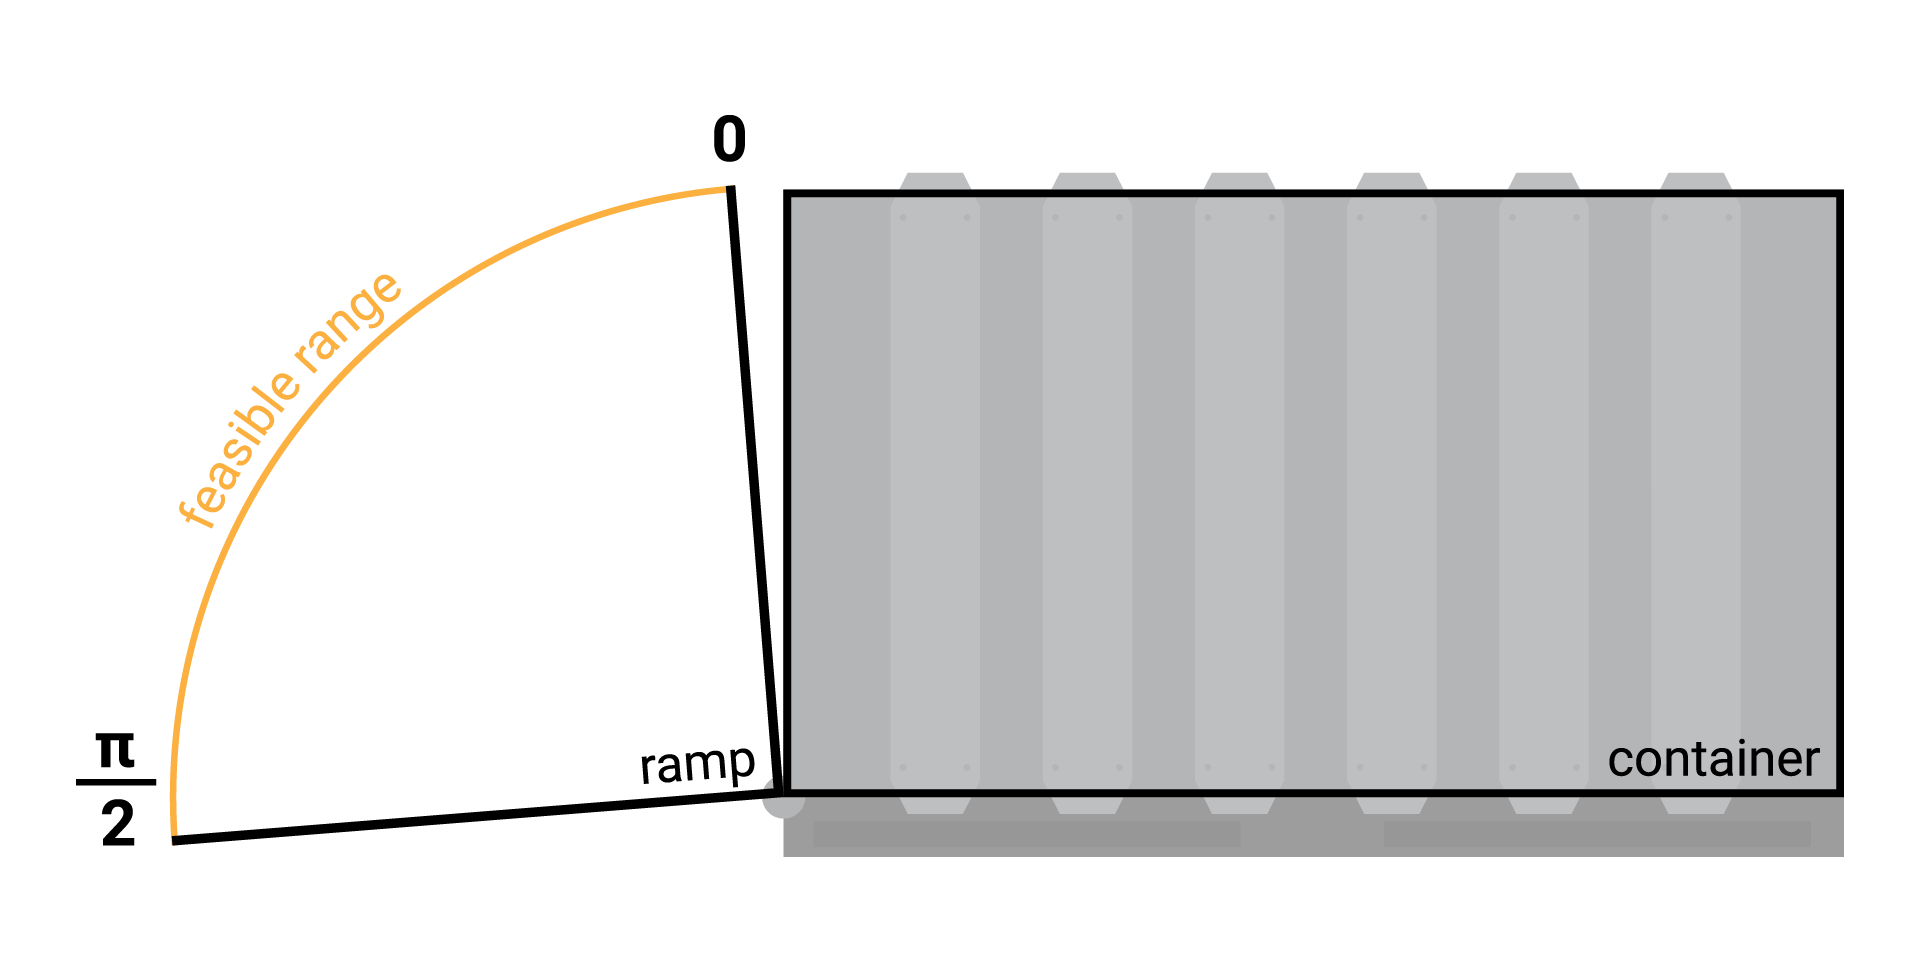
\includegraphics[width=0.75\textwidth]{img/joint_position_container.png}
    \caption{\textsc{Joint Positions of the Entrance Ramp}}
    \label{fig:joint_positions}
\end{figure}
\noindent
A closed container case could in principle also be detected by the navigation monitoring solution described in section \ref{sec:sim_and_mon_navigation_failures}, but such situations
are also recognized by the docking state machine, which returns an error after several entry attempts. Therefore, it is not determined which monitoring procedure is triggered first,
as this depends on the situation and environment, but generally one of the two nodes will be triggered and initiate resolution. Undocking errors are in principle not very diverse,
since it is only a question of leaving the container. They can therefore be simulated simply by a raised ramp, so that the robot is locked inside the container. This is in turn achieved
by publishing $j = 0$ to \code{/container/ramp_position_controller/command} while the robot is inside the container. To ensure that the robot is actually inside the container when
this case is simulated, the execution of the simulation does not follow immediately after initiation, but waits until the next \code{charge} action indicated by the operation
state machine is executed. A noteworthy aspect of the \textquote{ramp-based} simulations is that the robot cannot solve the problem itself. Ultimately, a failed charge is also quite trivial to simulate
based on a controllable battery consumption and recharge model. Charging failure simulation can be enabled using the following ROS topics:
\begin{itemize}
    \item \textbf{undocking failure (raised ramp):} \code{/sim_undocking_failure}
    \item \textbf{docking failure (raised ramp):} \code{/sim_docking_failure_raised_ramp}
    \item \textbf{docking failure (wrong base pose):} \code{/sim_docking_failure_base_pose}
    \item \textbf{charging failure:} \code{/sim_charging_failure}
\end{itemize}
These issues can be addressed with the resolution methods described in section \ref{sec:charging_failure_resolver}.

\subsection{Drastic Weather Change}
\label{sec:sim_and_mon_drastic_weather}

There are two ways to incorporate weather information, either by having the robot detect it with its own sensors or by utilizing external weather information. In any case,
it would be good to identify extreme weather conditions that could affect the proper functioning of the system in order to react accordingly, i.e., return to the base station and
seek shelter. Since we live in a world where local weather information is quite readily available and the robot's sensing capabilities would also be limited in its ability to
reasonably detect it, external weather information is used. In addition, realistic simulation of weather phenomena is a difficult task that would shift the focus of the work.
Thus, the robot does not detect extreme weather conditions itself through its sensors, but relies on external local weather data. To retrieve local weather information, a \textit{Python}
wrapper of the \textit{OpenWeatherMap} API\footnote{\textcolor{link-color}{\url{https://openweathermap.org/api}}} is used, guaranteeing cross-platform applicability.\newline

\noindent
Initially, the weather monitoring node
establishes a connection to the \textit{OpenWeatherMap} API. If successful, it continuously requests local weather data at a user-configurable frequency, e.g., every half hour.
As weather data should be based on the current location of the robot, the node maintains a subscription to the \code{/fix} topic described in section
\ref{sec:sim_and_mon_gnss_connection_problems}, through which \code{NavSatFix}\footnote{\textcolor{link-color}{\url{https://docs.ros.org/en/api/sensor\_msgs/html/msg/NavSatFix.html}}} messages containing the latitude and longitude of the robot's currently presumed position arrive as
new GNSS data is made available. These coordinates are used to retrieve local weather information from the \textit{OpenWeatherMap} API. After parsing the data relevant for
monitoring, the actual monitoring at the user-specified frequency begins.\newline
First, the current rain volume $r_v$ in $mm/h$ is monitored based on two cases: If $7.6 > r_v > 2.6$,
the rain is considered moderate and manageable, so an information is published to the operator, but the robot continues its work. When $r_v \geq 7.6$, the rain is considered heavy,
causing the robot to interrupt its mission and launch a contingency. This classification of precipitation intensity stems from the \textit{American Meteorological Society's
Glossary of Meteorology}\footnote{\textcolor{link-color}{\url{https://glossary.ametsoc.org/wiki/Rain}}}. Analogously, the current snow volume $s_v$ is monitored in $mm/h$. When $2.0 > s_v > 0.5$, it is
considered bearable and only the operator is informed about the situation, but if $s_v \geq 2.0$, an interruption of the work is initiated. The next aspect monitored is the wind speed,
where \textit{OpenWeatherMap} distinguishes between a general wind speed and a gust speed. The former refers to a prolonged wind speed and the latter to sudden gusts of wind.
Since both can be dangerous for the operation of the robot, they are monitored together and summarized as wind speed $w_s$ in $m/s$ in the following. If $14.0 > w_s > 11.0$, the
robot continues its work but informs the operator of a \textquote{strong breeze}. When $20.0 > w_s \geq 14.0$, the robot still continues its work, but informs the operator of a gale
and that it is starting to get critical. When $28.0 > w_s \geq 20.0$, the robot interrupts its mission and informs the operator of a strong gale and the risk of structural damage.
Moreover, at $33.0 > w_s \geq 28.0$, the robot reports a storm force and a very high risk of structural damage and aborts its mission. Finally, at $w_s \geq 33.0$, it aborts its operations
and reports a hurricane and a very high risk of severe and extensive structural damage. Wind speed classification limits are based on wind speed estimates from the \textit{US Department of
Commerce's National Weather Service}\footnote{\textcolor{link-color}{\url{https://www.weather.gov/pqr/wind}}}. Furthermore, the temperature is monitored in \textdegree{}C based on $t_{min}$ and $t_{max}$,
the minimum and maximum temperatures measured in the robot's further surroundings, as well as $t$, the current temperature at the robot's location. It is reasonable to assume both
an upper and a lower limit for the temperature in the robot's working environment. As such lower and upper bounds depend heavily on the robotic system in question as well as its
sensor equipment, the limits are user-configurable. By default, a contingency due to excessive temperatures is initiated when $t > 40$ or $t_{max} > 40$. Likewise, the robot
interrupts its mission due to extreme cold when $t < -5$ or $t_{min} < -5$, e.g., because this could be problematic for the system's battery. The \textit{OpenWeatherMap} API
additionally provides a weather condition code\footnote{\textcolor{link-color}{\url{https://openweathermap.org/weather-conditions}}} for each situation, which is well-suited for systematic monitoring.
Based on these codes, it is easy to interrupt the mission for all possible variants of thunderstorms. Besides the specific checks for precipitation amounts mentioned above,
there are also codes for variations of heavy rain and snow that are used as indicator for contingencies. Additionally, codes for squalls, tornados, and atmospheric features
such as mist, smoke, or fog are used to interrupt the mission. Eventually, the \textit{OpenWeatherMap} information also contains the sunrise and sunset times. Since the robot
requires daylight for its missions, it also interrupts them when it approaches or even exceeds sunset or when it tries to start before sunrise. As anticipated in section
\ref{sec:lta_problems_not_considered}, the inclusion of this information covers the neglected problem category of \textquote{certain dynamics}, at least in this sense.\newline
Of course, all upper and lower bounds
for the attributes of the current weather situation are in principle configurable by the user, but are set to reasonable default values from the literature.
In all contingency
cases, the weather monitoring node publishes a message on the \code{/contingency_preemption} topic indicating the particular type of weather condition and causing a transition to
the \code{CONTINGENCY} state where an appropriate resolution method is selected and launched. Afterwards, it transitions to a kind of passive monitoring mode where it no longer
triggers contingencies etc., but only waits until the weather situation is moderate again and reports this on the topic \code{/moderate_weather}. In addition, it listens to a
topic where the resolver provides its results. If successful, the weather monitoring transitions to active monitoring again.
Similarly, the information that does not require interruption of the mission is transmitted via the \code{/robot_info} topic. Aside from the
information relevant to monitoring, there is some other information that may be of interest to the operator. Therefore, a full weather report can be configured to be communicated
to the operator at specified intervals, e.g., once a day. Beyond those already discussed, this information includes observation time, a general status description, the cloudiness
percentage, the humidity, the atmospheric pressure and the wind direction.\newline
In order for a system to utilize the weather monitoring node, it should provide \code{NavSatFix} data on
the \code{/fix} topic, as the weather information is based on the current location of the robot. Alternatively, the values for latitude and longitude can be configured explicitly.
Furthermore, an internet connection is required to connect to the \textit{OpenWeatherMap} API.\newline

\noindent
As always, in order to evaluate the monitoring procedures, a simulation of the various scenarios must be provided. This simulation takes place in the parser for
\textit{OpenWeatherMap} data. Based on the developed weather monitoring node, it is fairly trivial to simulate the occurrence of such extreme weather conditions by simply setting
the attributes to extreme values, e.g., a heavy rain scenario can be simulated by setting the corresponding rain volume $r_v = 8$. Likewise, a heavy snow situation can be simulated
by setting $s_v = 3$. The simulation of the remaining extreme weather events can be triggered analogously. Weather-related challenges for LTA can be dealt with using the resolver
described in section \ref{sec:weather_resolver} and the simulation of extreme weather events can be activated / deactivated via the following ROS topics:
\begin{itemize}
    \item \textbf{heavy rain:} \code{/toggle_rain_sim}
    \item \textbf{heavy snow:} \code{/toggle_snow_sim}
    \item \textbf{gale:} \code{/toggle_wind_sim}
    \item \textbf{low temperature:} \code{/toggle_low_temp_sim}
    \item \textbf{thunderstorm:} \code{/toggle_thunderstorm_sim}
    \item \textbf{sunset:} \code{/toggle_sunset_sim}
\end{itemize}

\subsection{Sensor (Perception) Failure}
\label{sec:sim_and_mon_sensor_failures}

Since the scenario described in section \ref{sec:prototype_scenario} assumes a representation of a \code{scan} action, but the work does not really depend
on realistic scan data, a pragmatic solution for the simulation is required. The result is the dummy scanning node introduced in section \ref{sec:dummy_scanning_node}.
The actual monitoring and simulation of sensor failures is described in the subsequent section \ref{sec:sensor_mon_and_sim}.

\subsubsection{Dummy Scanning Node}
\label{sec:dummy_scanning_node}

The dummy scanning node implements a ROS \code{SimpleActionServer}\footnote{\textcolor{link-color}{\url{http://wiki.ros.org/actionlib}}} that simulates the results of the
\textit{RIEGL} lidar sensor (cf. fig. \ref{fig:arox_system}).
It is expected that a \code{scan} action will trigger an incoming \code{LaserScan} on the topic \code{/RIEGL}, which will then be
written to a file to also have some form of data management. Since the \textit{Velodyne} lidar sensor (cf. fig. \ref{fig:arox_system}) is already part of the simulation and the nature of the incoming data
is essentially the same, a \code{scan} action just leads to one republished \textit{Velodyne} scan under the \code{/RIEGL} topic using \code{rospy.wait_for_message()},
which merely creates a subscription to the topic, receives one message, and then unsubscribes. The incoming data is basically a list of distance values for certain angle-height 
combinations along with arbitrary many metadata such as minimum angle, maximum angle, scanning time, and identifier. Thus, the dummy node enables the \textit{Velodyne} sensor
to briefly pretend to be a \textit{RIEGL} sensor. This approach has the useful side effect of making it relatively easy to simulate sensor failures by simply stopping to
republish the \textit{Velodyne} after a \code{scan} action.\newline
The actual real \textit{RIEGL} sensor scans are of data type \code{PointCloud2}, and the monitoring solutions described in section \ref{sec:sensor_mon_and_sim}
are capable of processing incoming scans of types \code{LaserScan} as well as \code{PointCloud2}. It is configurable in which form the data should be received. 
Generally, the sensor can make the scans available to the ROS system via a topic, i.e., the sensor publishes the scans, e.g., on \code{/RIEGL}.

\subsubsection{Monitoring and Simulation of Sensor Failures}
\label{sec:sensor_mon_and_sim}

Obviously, total sensor failures are realistic in practice for any lidar sensor, or even any sensor in general, due to a hardware fault, an interrupted
power supply, or a variety of other reasons. Yet, there are more subtle failures than just a total breakdown, and the incoming scan data should be checked for plausibility.
From a practical point of view, it is a valid assumption to receive the scans via a specific ROS topic. One issue could be an empty list of range values, i.e., a scan arrives on
some ROS topic but is essentially vacuous. As mentioned in section \ref{sec:dummy_scanning_node}, the crucial part of a laser scan is the list of range values, which makes it 
useless if this list is empty for some reason. Its realism could be debated, and of course it is pointless to detect issues that do not occur in practice. However, since it is
relatively easy to simulate and detect, it is treated as a basic test that can be used, for example, to detect problems due to implementation-specific errors.
Another, more subtle problem could be a scan that mainly contains values that do not satisfy the sensor's maximum or minimum range, i.e., \code{inf}, which may indicate that
the robot has fallen over, or the sensor has slipped out of position. This could indicate, for example, that the sensor is pointing towards the sky, causing the values to exceed
the maximum range. Though, depending on the sensor used and the environment, in large open fields the nearest objects that could be detected may actually be farther away and exceed
the maximum range of the sensor. Analogously, the same problem occurs if an object is too close to the sensor, i.e., the minimum range is undercut. In both cases, the sensor only
returns \code{inf} values. It should be detected when the list of range values is predominantly filled with impermissible \code{inf} values. Finally, it could be a problem if the
same scan is published repeatedly. It is possible that the range values between two scans where the robot has not moved are similar, although they should never be the same due to
noise, etc. However, what should be different in each case is the metadata such as the ID.\newline

\noindent
Executing a \code{scan} action not only launches the dummy scanning node introduced in section \ref{sec:dummy_scanning_node}, but also a monitoring procedure that
looks for potential problems with the laser scanner. The most obvious type of sensor failure is of course a total failure, i.e., no messages arrive on the corresponding ROS topic.
A fairly trivial approach to detecting total sensor failures is therefore to use \code{rospy.wait_for_message()} with the particular topic and set a time limit $t \in \mathbb{N}$
in seconds after which a missing scan is considered a total sensor failure. Of course, such a timeout is highly dependent on the respective application and also on the sensor 
configuration, since a higher angular resolution naturally requires a longer runtime, e.g., a longer runtime due to a higher resolution should not be falsely identified 
as sensor failure. In addition, there could be different modalities of recording with the sensor. The scan can be recorded continuously or published in parts.
Therefore, the time limit $t$ is configurable by the user. While trivial, such a monitoring is not yet available and is critical for reasonable long-term autonomy in the 
considered scenario described in section \ref{sec:prototype_scenario}. In summary, whenever the runtime $r \in \mathbb{N}$ of a scan recording exceeds the user-specified time
limit $t$, i.e., $r > t$, a total sensor failure is assumed. Nonetheless, more subtle errors should also be detected, beyond the outright absence of scans.
For this purpose, the incoming scans must be examined more closely and checked for plausibility. For example, if the list of range values is empty, it is as useless for
the mission as a scan that does not arrive at all. Hence, after the arrival of a new scan, the monitoring solution verifies that the list of range values is not empty.
Another interesting issue to detect is a list of range values that predominantly contains \code{inf} values, which, as mentioned before, could indicate that the sensor is
pointing towards the sky, e.g., because the robot has fallen over,
or the sensor has slipped. Admittedly, it would be a bit too simplistic to consider only range lists entirely filled with \code{inf} values as problematic.
In many cases, depending on the field of view, the sensor can still receive reasonable values if it is oriented towards the sky, for example.
In the minimal simulation scenario with the AROX (see section \ref{sec:prototype_scenario}), the \textit{Velodyne} scanner still receives about $10$\% of 
reasonable-looking range values when the robot is tilted on its back and the sensor is pointing toward the sky, as shown in figure \ref{fig:tilted_AROX}.
As can be seen in figure \ref{fig:straight_line}, in such a case the sensor detects parts of the ground on both sides of the robot as well as parts of the 2.5D 
representation of a hedge in the background. Accordingly, it makes much more sense to let the user define a lower bound for reasonable-looking values (non-\code{inf}),
e.g., that depending on the scenario and sensor configuration, at least $10$\% of the detected values must be non-\code{inf} for the scan to be considered feasible.
\begin{figure}[H]
    \centering
    \begin{subfigure}[b]{0.49\textwidth}
        \centering
        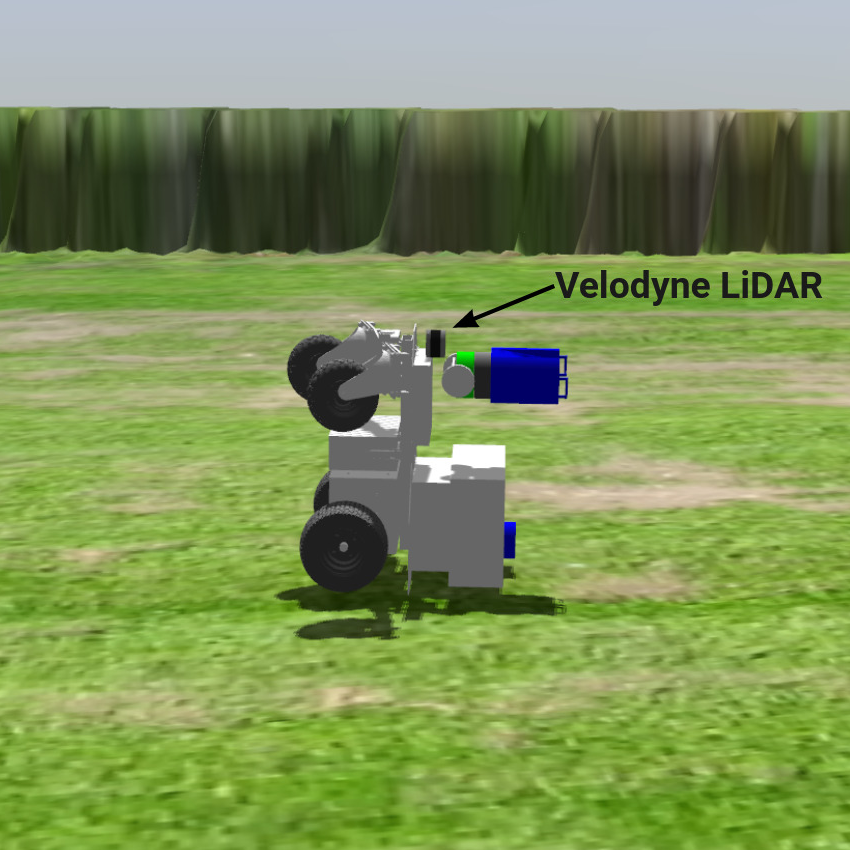
\includegraphics[width=0.65\textwidth]{img/tilted_AROX.png}
        \caption{\textsc{Tilted AROX in Simulation}}
        \label{fig:tilted_AROX}
    \end{subfigure}
    \hfill
    \begin{subfigure}[b]{0.49\textwidth}
        \centering
        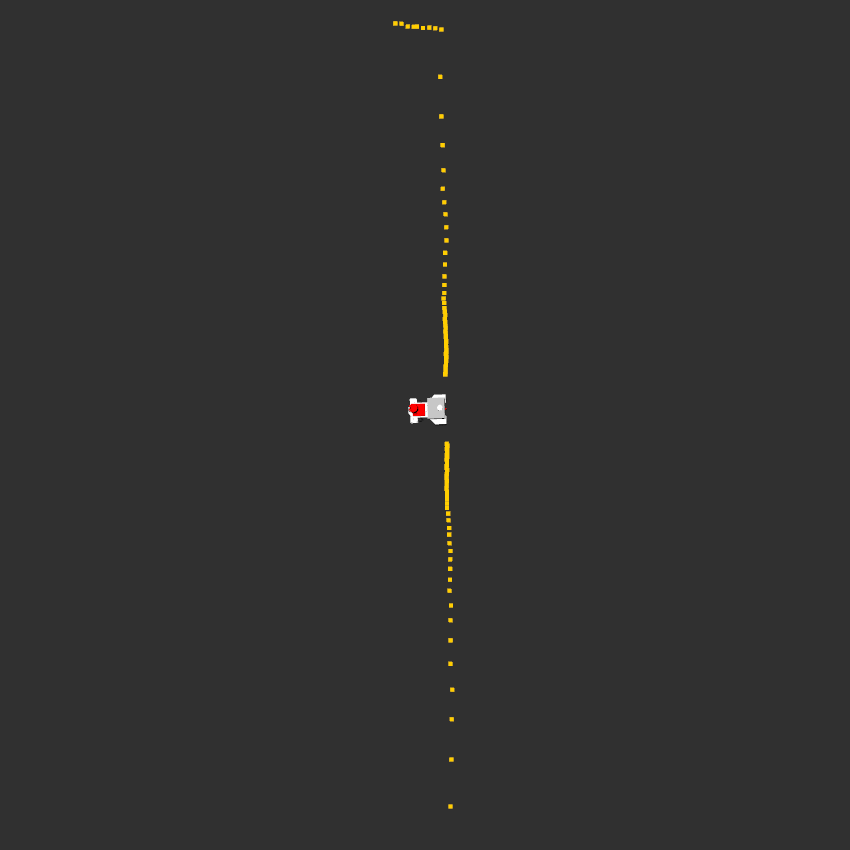
\includegraphics[width=0.65\textwidth]{img/straight_line.png}
        \caption{\textsc{Feasible Range Values when Facing the Sky}}
        \label{fig:straight_line}
    \end{subfigure}
\caption{\textsc{Experiments with Tilted Sensor}}
\label{fig:prototype_sim}
\end{figure}
\noindent
The monitoring solution implements this approach by calculating the ratio between feasible and infeasible values and comparing it to the lower bound.
If the percentage of feasible range values does not exceed the lower bound, it is considered a sensor failure.
Moreover, it should be detected when no new scans arrive, i.e., the received scan is repeatedly the same.
To be able to compare the newly arrived scan with the previous one, the monitoring node always saves the last scan.
For the actual comparison, a unique hash value is calculated for both scans based on their range values as well as various metadata such as timestamp,
frame identifier, minimum and maximum angle, angle increment, time increment, scan time, and minimum and maximum range.
If the newly arrived scan has the same hash value as the previous one, such a sensor error has been detected.
It is crucial to keep the monitoring solutions as general as possible, i.e., abstract from the specific sensors (\textit{RIEGL}, \textit{Velodyne})
in order to make them reusable for others. One hurdle standing in the way of this claim is the fact that many sensor manufacturers use their own proprietary data types.
Nevertheless, the underlying data is likely to be very similar. To provide some generality, the developed monitoring approaches will be able to handle the two data 
types commonly used in the ROS ecosystem, \code{LaserScan} and \code{PointCloud2}. In all cases, the sensor monitoring node publishes on the topic
\code{/contingency_preemption} with a message that specifies the particular kind of sensor failure and causes a transition to the \code{CONTINGENCY} state.
For a system to use the sensor monitoring node, it must indicate a scan action by publishing on the \code{/scan_action} topic. Additionally, the topic under which the
\code{LaserScan} or \code{PointCloud2} is expected must be configured.\newline

\noindent
The evaluation of a total sensor failure is straightforward, as it can be easily simulated by interrupting the publication of laser scans in the dummy scanning node
described in section \ref{sec:dummy_scanning_node}. The second identified type of sensor failure, i.e., an empty list of range values, is again rather trivial to simulate
by clearing the list of range values before republishing a scan in the dummy scanning node. Scans consisting mainly of impermissible range values can be realized by 
simply manipulating the range values of a scan so that they do not satisfy the maximum and minimum range of the sensor before republishing, i.e., \code{inf}.
Finally, to simulate repeated scans, the dummy scanning node always stores the previous scan and can replace the current scan with the previous one on command.
Accordingly, the simulation of each different sensor fault case is implemented as part of the dummy scanning node introduced in section \ref{sec:dummy_scanning_node},
and can be enabled / disabled via the following ROS topics:
\begin{itemize}
    \item \textbf{total sensor failure:} \code{/toggle_simulated_total_sensor_failure}
    \item \textbf{empty list of range values:} \code{/toggle_simulated_empty_ranges}
    \item \textbf{predominantly impermissible values:} \code{/toggle_simulated_impermissible_ranges}
    \item \textbf{repeated scan:} \code{/toggle_simulated_scan_repetition}\newline
\end{itemize}
Sensor failures of this kind can be addressed with the resolution methods described in section \ref{sec:sensor_failure_resolver}.

\subsection{Lost Connection}
\label{sec:sim_and_mon_lost_connections}

Monitoring and simulation of the specific types of considered connection failures, i.e., WiFi (cf. sec. \ref{sec:sim_and_mon_wifi_connection_problems}), internet
(cf. sec. \ref{sec:sim_and_mon_internet_connection_problems}) and GNSS (cf. sec. \ref{sec:sim_and_mon_gnss_connection_problems}) connection problems,
are part of the following sections. However, there is also one monitoring aspect that works identically for all three, namely timeout monitoring. There is a continuously running
procedure that checks the time since the last message from either connection. If a user-specified time limit for one of the connections is exceeded, a contingency 
due to a disconnection is initiated. In general, connection failures can be addressed with the resolution methods described in section \ref{sec:connection_resolver}.

\subsubsection{WiFi Connection Failures}
\label{sec:sim_and_mon_wifi_connection_problems}

The most common form of WiFi failure, which is very relevant and realistic in practice, is of course a simple disconnection.
However, there are again more subtle challenges than just the complete absence of a connection, so the quality of an established connection should also be monitored.
Generally, network monitoring can be done arbitrarily detailed, for this work it is limited to some attributes that allow a general statement about the quality of
the connection in practice. One realistic problem is an overall poor link quality, which is a measure combining different kinds of metrics, e.g.,
\textit{Received Signal Strength Indication} (RSSI), \textit{Signal to Interference plus Noise Ratio} (SINR), \textit{Packet Delivery Ratio} (PDR), and
\textit{Bit Error Rate} (BER). \cite{Vlavianos:2008} Another well-known issue with WiFi systems is a poor signal, i.e., a low RSSI value. The RSSI is already part of
the link quality assessment, but due to its practical importance, it is also worth to be considered in isolation. Furthermore, the bit rate, i.e., the speed at which
information is transmitted, gives a good indication of the overall connection quality, and it should be recognized when it falls below a certain threshold, which is a
lower limit for practical use. In order to ensure communication with the base station at all times (RTK correction signals, scan storage, etc.), such problems should be
detected and reported or corrected immediately.\newline
Of course, the WiFi connection is context-dependent and should be very strong in the proximity of the base station, while it can
be arbitrarily weak out in the field. Nevertheless, for the scenario under consideration, it is assumed that it is available at all times in a certain quality. If this is not the
case in other scenarios, the thresholds can be reconfigured and, if WiFi is not expected to be available at all, the monitoring node can be disabled.\newline

\noindent
Monitoring for WiFi connectivity issues takes place at two levels of abstraction. From the perspective of the high-level execution monitoring framework developed in this work,
the monitoring is completely independent of hardware and operating system details. However, monitoring the WiFi connection of a particular system depends heavily on such details,
so it is also necessary to provide low-level monitoring for network interfaces. The idea is that the high-level monitoring node expects the information that are evaluated as part 
of the monitoring in a very specific format on the ROS topic \code{/wifi_connectivity_info}. For this purpose, a custom ROS message \code{WiFi.msg} was defined consisting of the
three fields \code{float32 link_quality}, \code{float32 signal_level} and \code{float32 bit_rate}. Therefore, it is irrelevant where this information comes from, it is simply
assumed to be provided. In order to demonstrate the WiFi monitoring in this work, the low-level operating-system-specific monitoring node that transfers this
information to the ROS system is implemented exemplarily for an Ubuntu system. It starts the Unix tool \code{iwconfig}
\footnote{\textcolor{link-color}{\url{https://manpages.debian.org/bullseye/wireless-tools/iwconfig.8.en.html}}} as a subprocess for a WiFi interface identifier that can be configured by the user. Subsequently,
the relevant information, i.e., link quality, signal level and bit rate, is parsed from the \code{iwconfig} output for the respective interface and a \code{WiFi.msg} is created
based on this. This message is then published under the \code{/wifi_connectivity_info} topic, which is subscribed by the high-level monitoring node. This process is repeated
continuously every $10$s.\newline

\noindent
Now that it is clear how the low-level node works, the actual monitoring follows. As mentioned, the high-level monitoring node receives the WiFi information via
\code{/wifi_connectivity_info}. Based on this, the numerical information about the connection is evaluated. If all three provided values are $0$, it is considered
a disconnect and the monitoring solution induces a transition to the \code{CONTINGENCY} state. The link quality is evaluated based on three thresholds: If it is below $5\%$,
it is considered critically poor quality and a transition to \code{CONTINGENCY} follows. For the remaining two thresholds, the quality is not as bad as requiring a contingency
case, but it is still worth notifying the operator. For a link quality of less than $25\%$ a poor quality is reported, and for values less than $50\%$ a below average quality.
The second attribute, the RSSI, ranges from $-30$ dBm to $-100$ dBm, depending on various aspects such as distance. \cite{Heurtefeux:2012} The upper bound of $-30$ dBm is the
optimal value, which is almost impossible to achieve in practice, and $-100$ dBm basically means no signal at all. One could roughly classify it as follows: Anything between the
optimal $-30$ dBm and $-67$ dBm can be considered very good in practice, below an RSSI of $-80$ dBm it starts to become critical, and around $-90$ dBm it becomes practically 
unusable. \cite{metageek} Accordingly, the RSSI is also monitored based on three thresholds. As it becomes practically unusable for values below $-90$ dBm, $-90$ dBm acts as a
threshold for contingency cases, i.e., a lower bound. Signal levels of $\leq -80$ dBm and $\leq -75$ dBm cause notifications of very weak and weak WiFi signals,
respectively. Finally, the bit rate is monitored based on two cases: If it is below $1$ Mb/s, a contingency is triggered, and if it is below $20$ Mb/s, a notification of a
rather low bit rate is transmitted. Since the question of which values are considered problematic here depends heavily on the environment and application scenario, these values
are configurable by the user. As soon as a malfunction is detected, monitoring is deactivated and resumed only when the issue has been solved. In all contingency
cases, the high-level WiFi monitoring node publishes on the topic \code{/contingency_preemption} with a message that specifies the particular kind of connection problem.\newline
In summary, the problem of actually detecting the WiFi connectivity on the system in question is completely external to the execution monitoring framework,
which has no operating system coupling at all. There is a layer of abstraction that separates the two views. The assumption of the high-level monitoring framework is the
following: There is a node that publishes the WiFi connectivity for the system every $10$s in the \code{WiFi.msg} format on \code{/wifi_connectivity_info}. If someone wants to use
the execution monitoring framework on Windows, for instance, there is no need to modify the framework's code, there just has to be an equivalent WiFi monitoring node for a Windows
system that replaces the Ubuntu-specific one.\newline

\noindent
The simulation of WiFi connection failures is realized by the operating-system-specific implementation of a WiFi monitoring node described above.
The idea is to simply publish problematic values for each of the considered attributes of the WiFi connection,
i.e., link quality, signal level and bit rate. The simplest case of a complete disconnection is simulated by setting all three values to $0$.
A poor link is simulated by publishing a corresponding value of $2\%$, meaning that the measure of how good the link is described above estimates the quality
with only two percent of the optimum. 
A signal level failure is simulated by publishing an RSSI value of $-90$ dBm. Finally, the default value for a simulated bit rate failure 
is $0.1$ Mb/s. The simulation of each different WiFi fault case can be enabled / disabled via the following ROS topics:
\begin{itemize}
    \item \textbf{poor link quality:} \code{/toggle_simulated_bad_wifi_link}
    \item \textbf{poor signal level:} \code{/toggle_simulated_bad_wifi_signal}
    \item \textbf{poor bit rate:} \code{/toggle_simulated_bad_wifi_bit_rate}
    \item \textbf{disconnection:} \code{/toggle_simulated_wifi_disconnect}
\end{itemize}

\subsubsection{Internet Connection Failures}
\label{sec:sim_and_mon_internet_connection_problems}

Unlike monitoring WiFi connectivity, internet connectivity monitoring does not require an operating system specific low-level node. The internet bandwidth is tested using the
cross-platform \textit{Python} tool \code{speedtest-cli}\footnote{\textcolor{link-color}{\url{https://pypi.org/project/speedtest-cli/}}}. Nevertheless, for modularization reasons, there is a separate internet
connectivity monitoring node that communicates the internet connectivity properties to the general connectivity monitoring node via the ROS topic \code{/internet_connectivity_info}.
For this purpose, a custom ROS message \code{Internet.msg} was defined consisting of the two fields \code{float32 download_speed} and \code{float32 upload_speed}.\newline

\noindent
Initially,
the connection to the \code{speedtest-cli} API is established. If this fails, an exception is caught and the first type of internet connection problem is detected, namely a
complete disconnect. In such a case, the internet monitoring node creates and publishes an \code{Internet.msg} consisting of an upload and download speed of $0$ Mb/s
reflecting cases of real disconnects after a successful connection to the API. On the other hand, if the connection to the API is successful, the actual monitoring begins, which
repeatedly performs speed tests every $n \in \mathbb{N}$ seconds, where $n$ can be configured by the user. For each result, the download and upload speed is parsed and an \code{Internet.msg} is
generated and published. The high-level connectivity monitor receiving the message performs several checks based on the data. In addition to a check for complete disconnects,
i.e., upload and download of $0$ Mb/s, which causes a contingency, other specific checks are performed. When the download speed $d < 1$ Mb/s, a critically low download speed is 
detected and a contingency is initiated. If $d < 40$ Mb/s, an information is sent to the operator that a rather low download speed was detected. Analogously, the upload speed $u$ is
checked. An upload speed of $u < 1$ Mb/s causes a contingency, and $u < 10$ Mb/s initiates an information of a rather poor upload speed in the communication channel with the human
operator. As always, in all contingency cases, the monitoring node publishes a message on \code{/contingency_preemption} that specifies the particular nature of the connection
problem. In cases of a failed connection to the \code{speedtest-cli} API, the monitoring itself does not work properly, so the connection is reinitialized after the problem is fixed.\newline

\noindent
Simulating internet connectivity problems has three components. First, a total disconnect, which can be simulated by simply cutting the connection or publishing on a prepared topic.
The other two options are again simulated by publishing user-configurable problematic values for the respective download and upload speed components.
By default, a poor download as well as upload speed is simulated by publishing corresponding values of $0.5$ Mb/s.
The simulation of poor download and upload speed cases as well as a total failure can be enabled / disabled via the following ROS topics:
\begin{itemize}
    \item \textbf{disconnect:} \code{/sim_internet_connection_failure}
    \item \textbf{poor download speed:} \code{/toggle_simulated_bad_download}
    \item \textbf{poor upload speed:} \code{/toggle_simulated_bad_upload}
\end{itemize}

\subsubsection{GNSS Connection Failures}
\label{sec:sim_and_mon_gnss_connection_problems}

Unlike the connections considered in the previous two sections, i.e., WiFi and internet (cf. sections \ref{sec:sim_and_mon_wifi_connection_problems} and
\ref{sec:sim_and_mon_internet_connection_problems}), GNSS signals are already part of the ROS world both in the prototype simulation and in practice. The transmission of GNSS data
for both scenarios is shown in fig. \ref{fig:gnss_communication}, where the blue arrows represent the procedure in practice and the red arrows illustrate the case of simulated GNSS
data. In practice, the AROX system as well as the base station (mobile container) use a \textit{u-blox C099-F9P}
\footnote{\textcolor{link-color}{\url{https://www.u-blox.com/en/product/c099-f9p-application-board?lang=de}}} application board as GNSS receiver. The board can be configured to transmit or receive RTK correction
signals. Accordingly, the one on board the AROX is configured as RTK-rover and the one mounted inside the base station is configured as RTK-base. The board attached to the AROX is
connected to the on-board computer via USB. Since the on-board computer is an Ubuntu system, the Unix tool
\code{gpsd}\footnote{\textcolor{link-color}{\url{https://manpages.ubuntu.com/manpages/trusty/man8/gpsd.8.html}}} can be used, a daemon that can be configured to read the GNSS data from the connected
\textit{u-blox} board. Afterwards, the ROS community package \code{gpsd-client}\footnote{\textcolor{link-color}{\url{https://wiki.ros.org/gpsd\_client}}} serves as a bridge between the operating system and the
ROS world. It reads the GNSS data from \code{gpsd} and generates a \code{NavSatFix} message from it, the typical data type for GNSS data in ROS. This message is then published under
the \code{/fix} topic and used for localization, etc. In the simulation scenario (cf. red arrows in fig. \ref{fig:gnss_communication}), \code{GazeboRosGps}, a module from the ROS community package
\code{hector_gazebo_plugins} \footnote{\textcolor{link-color}{\url{https://wiki.ros.org/hector\_gazebo\_plugins}}}, is used to simulate GNSS data. It already generates a \code{NavSatFix} message with the
simulated data. However, it does not simulate every single relevant aspect of the GNSS data. It simulates the position and altitude of the robot in \textit{WGS84} coordinates and
also a GNSS velocity vector, but the status, service and covariance information are not generated. This is where the \code{GNSS Simulator} developed as part of this work comes
into play, acting as a \textquote{man-in-the-middle} to enrich the data coming from \code{GazeboRosGps}. For this purpose, it receives the \code{NavSatFix} message from the
\code{/fix_plugin} topic and enriches it with user-configurable service, status and covariance information. Finally, as in the real scenario in practice, a \code{NavSatFix} message
appears on the \code{/fix} topic. Thus, from the perspective of any component that uses the GNSS information, such as localization, it is not clear and also irrelevant whether the
data is real or simulated, the result is the same.

\vfill
\pagebreak

\begin{figure}[H]
    \centering
    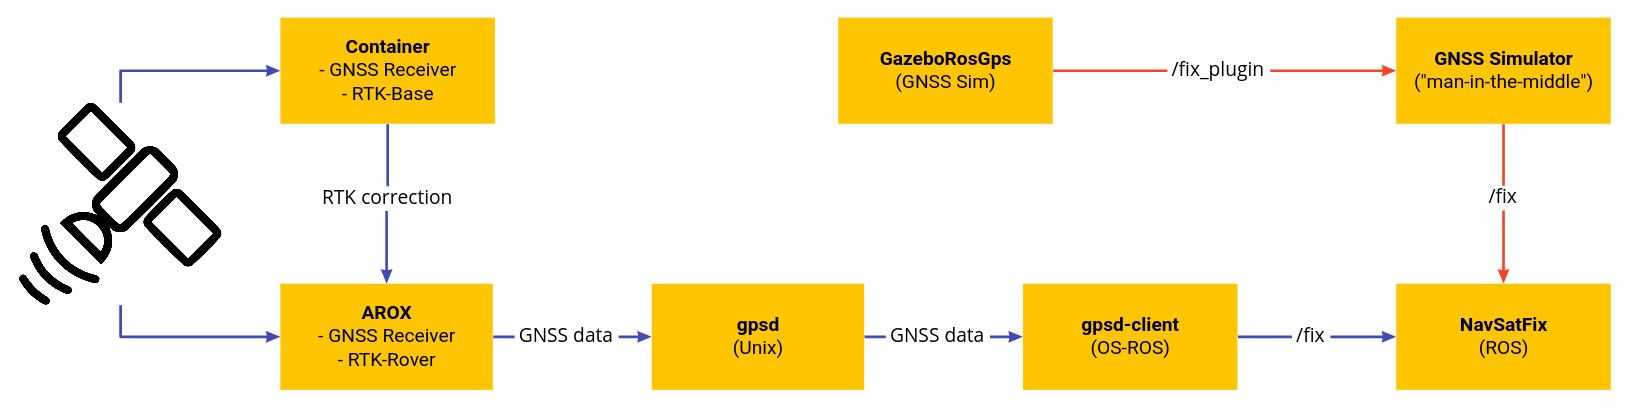
\includegraphics[width=\textwidth]{img/GNSS_comm.png}
    \caption{\textsc{Processing of GNSS Data (\textbf{\textcolor{myblue}{Practice}} / \textbf{\textcolor{myred}{Simulation}})}}
    \label{fig:gnss_communication}
\end{figure}
\noindent
As can be observed in the processing scheme in fig. \ref{fig:gnss_communication}, the GNSS data arriving at the system,
i.e., received from \code{gpsd}, is already the data potentially corrected by RTK. What is received is the best result there is at the moment; if RTK is available, it will be used.
What is part of the \code{NavSatFix} definition and also available in \code{gpsd}, i.e., in practice, is the GNSS status with the four possible options \code{STATUS_NO_FIX} $(-1)$,
\code{STATUS_FIX} $(0)$, \code{STATUS_SBAS_FIX} $(1)$ and \code{STATUS_GBAS_FIX} $(2)$. The first two options indicate whether or not it was possible to find a position using pure GNSS, e.g.,
\textit{GPS}, \textit{GLONASS} or \textit{Galileo}. An SBAS (\textit{Satellite Based Augmentation System}) is a satellite-based system that provides additional real-time data from geostationary
satellites to refine the observations and increase the accuracy, e.g., \textit{StarFire\textsuperscript{TM}}. \cite{Dixon:2006} Hence, the third option indicates whether such
an SBAS was involved in positioning. Analogously, a GBAS (\textit{Ground Based Augmentation System}) aims to ensure integrity and increase accuracy
by using a ground infrastructure consisting of at least two GNSS receivers. \cite{GNSS_aug} Based on this, differential corrections are computed. The fourth option therefore
tells whether a GBAS was utilized during positioning. Essentially, RTK is a specific GBAS system used in practice with the AROX system and the base station. These four GNSS status
options are user-configurable in the \code{GNSS Simulator}. Regardless of whether in simulation or in the case of the real AROX in practice, with the setup described it is always
known if RTK data is currently being received.
Additionally configurable, part of the \code{NavSatFix} message, and given in practice is the service option, i.e., the actual GNSS service used to
retrieve the data, \textit{GPS}, \textit{GLONASS}, \textit{Compass} or \textit{Galileo}.\newline

\noindent
Eventually, the GNSS covariance type as well as the covariances themselves are part of a
\code{NavSatFix} message and thus configurable in the \code{GNSS Simulator}. Covariances are commonly represented as a square matrix $C$ containing the covariance $c_{ij}$ for each pair
of variables $i, j$ in the considered domain $D$. These matrices have the property of being symmetric, that is, the covariance $c_{ij} \in C$ is the same as the covariance 
$c_{ji} \in C$, and they are providing the variances of the variables on their diagonal, since the covariance $c_{ii}$ of each variable $i \in D$ with itself is equal to the variance of
that variable. The \code{NavSatFix} specification distinguishes different types of position covariances, essentially indicating their reliability.
First, \code{COVARIANCE_TYPE_UNKNOWN} $(0)$ if the GNSS receiver does not yield a quality estimate and the GNSS data should be treated with caution.
\code{COVARIANCE_TYPE_APPROXIMATED} $(1)$ means that the GNSS receiver does not provide covariance values, but instead supplies another quality estimate, such as \textit{Dilution of Precision}
(DOP). The covariance values are then approximated based on this estimate. If the GNSS receiver gives at least the variances or standard deviations of the individual measurements,
the type is \code{COVARIANCE_TYPE_DIAGONAL_KNOWN} $(2)$, since the diagonal contains the variances. For instance, assuming the GNSS receiver provides the variances, it is only necessary
to take the square root of the diagonal values to obtain the more meaningful standard deviations. Eventually, \code{COVARIANCE_TYPE_KNOWN} $(3)$ means that the GNSS receiver provides
a rather sophisticated error estimation with a complete covariance matrix of $3 \times 3$ values.\newline

\noindent
The covariances are not directly based on the
current latitude, longitude and altitude belief state, but based on a $2D$ approximation of a small region of the Earth's surface, a tangential plane through the currently believed
position. There are several local tangent plane systems, the specific one assumed in \code{NavSatFix} is the \textit{East-North-Up} (ENU) coordinate system. Using such a coordinate
system relative to a local origin has the advantage that it allows one to work with intuitive Cartesian coordinates. To give an example, let the locations considered be the 
\textit{Innovation Center Osnabrueck} (ICO) and the \textit{DFKI-Lab Niedersachsen}, shown in fig. \ref{fig:ICO_DFKI_map}. A typical GNSS receiver estimates positions in
geodetic coordinates - latitude (degrees), longitude (degrees) and altitude (meters), e.g., ICO $(52.287690, 8.018690, 63.0)$ and DFKI $(52.287863, 8.027347, 63.0)$.
Let the ENU representation be constructed with respect to the ICO location (cf. fig. \ref{fig:ICO_DFKI_ENU}). This location is the origin of the local coordinate system, i.e., the location where the tangential
plane meets the Earth's surface. The two-dimensional \textquote{east-north-plane}, together with the \textquote{up-axis} perpendicular to the Earth at the reference point, form
the local Cartesian coordinate system (cf. fig. \ref{fig:ICO_DFKI_ENU}). This is, of course, only an approximation that is feasible for relatively small areas, since the Earth's curvature would have to be taken
into consideration for larger areas. Now another location, for instance that of the DFKI, is considered. The ENU representation provides the information where this point
of interest is located in the local coordinate system in meters. The result of converting the geodetic coordinates of the DFKI to the ENU system ($590.7, 19.3, 0.0$), is displayed
in fig. \ref{fig:ICO_DFKI_ENU}, i.e., the DFKI is located $590.7 m$ east and $19.3 m$ north of the ICO site. In this case, both locations have the same height.
\begin{figure}[H]
    \centering
    \begin{subfigure}[b]{0.49\textwidth}
        \centering
        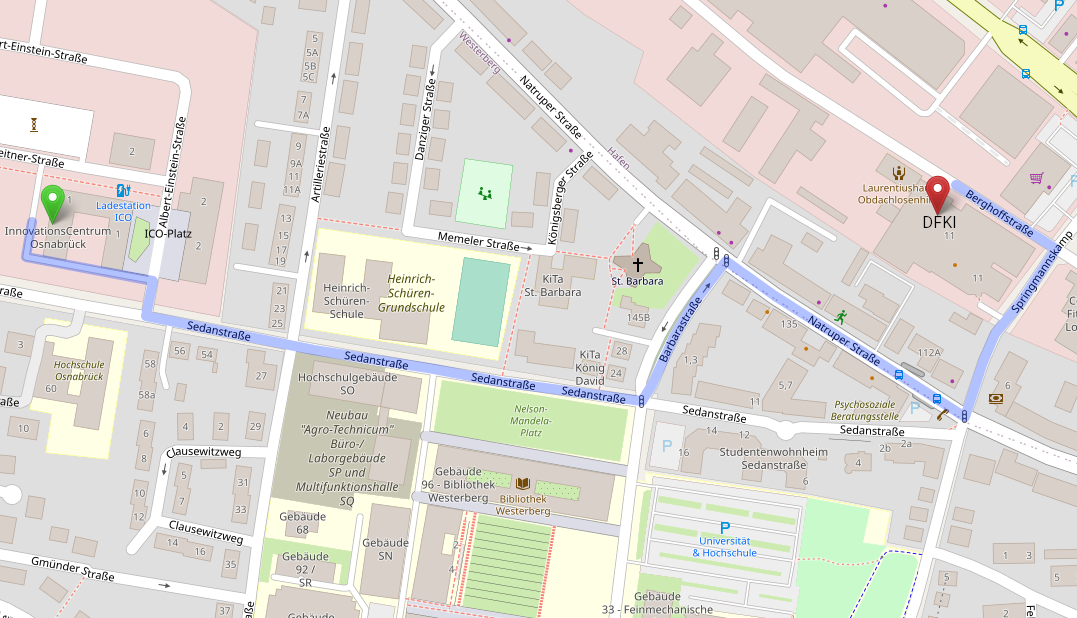
\includegraphics[width=\textwidth]{img/ICO_DFKI_map.png}
        \caption{\textsc{\textit{OpenStreetMap} Section}}
        \label{fig:ICO_DFKI_map}
    \end{subfigure}
    \hfill
    \begin{subfigure}[b]{0.49\textwidth}
        \centering
        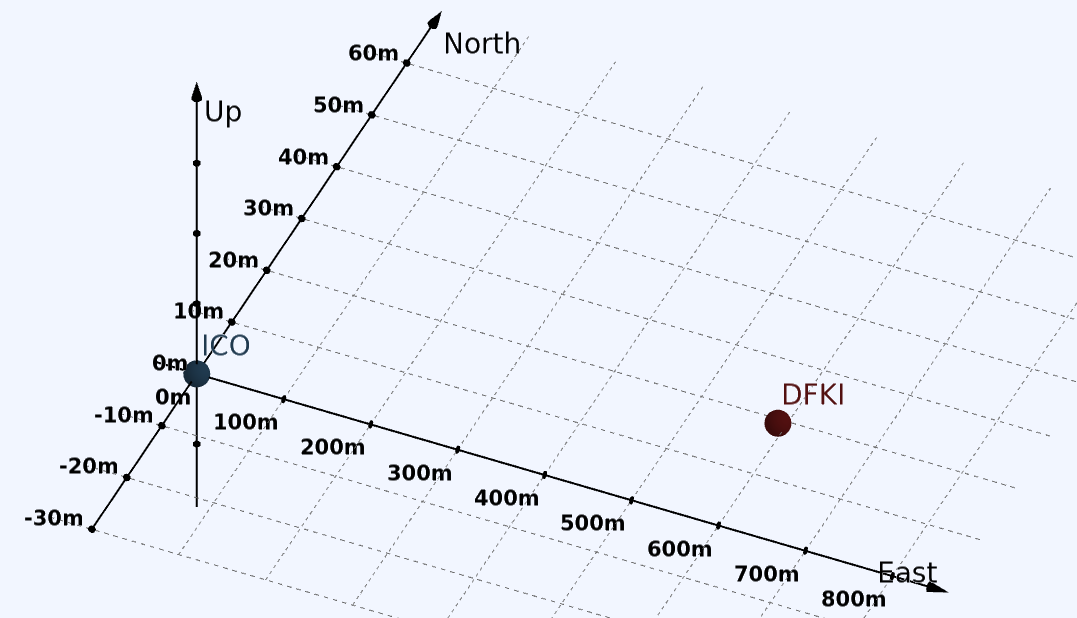
\includegraphics[width=\textwidth]{img/ICO_DFKI_ENU.png}
        \caption{\textsc{East-North-Up (ENU) Representation}}
        \label{fig:ICO_DFKI_ENU}
    \end{subfigure}
\caption{\textsc{Practical ENU Example}}
\label{fig:ENU_example}
\end{figure}
\noindent
The position covariances $C$ in a \code{NavSatFix} message are defined in square meters relative to the tangential plane.
The ENU system is composed of the three variables east ($E$), north ($N$) and up ($U$), i.e., $c_{ij} \in C_{3 \times 3}$ with $i, j \in \{E, N, U\}$.
Thus, one has to consider $\sqrt{c_{ii}} \thinspace \forall \thinspace i \in \{E, N, U\}$ to end up with the standard deviations in meters, i.e., how widely the GNSS approximations are
currently spread in meters. In general, a minor standard deviation implies that the uncertainty about the currently estimated position is very low, making the estimate very accurate.
Figure \ref{fig:low_uncertainty}, for instance, shows relatively low positional uncertainty based on standard deviations of $\sqrt{6}m$ in either direction. The violet shape
surrounding the AROX model indicates this uncertainty. In principle, the robot could be anywhere in this shape based on the current GNSS data, but the center is currently the most likely
estimated position (the average). Figure \ref{fig:high_uncertainty} shares the same standard deviations for the north and up directions, but has a significantly higher deviation of
$\sqrt{101}m$ in the east direction, resulting in a fairly high uncertainty with respect to this direction.
\begin{figure}[H]
    \centering
    \begin{subfigure}[b]{0.49\textwidth}
        \centering
        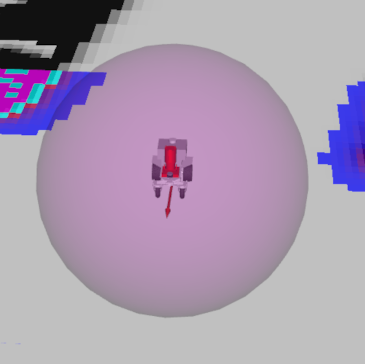
\includegraphics[width=0.75\textwidth]{img/GNSS_cov_low.png}
        \caption{\textsc{Relatively Low Uncertainty}}
        \label{fig:low_uncertainty}
    \end{subfigure}
    \hfill
    \begin{subfigure}[b]{0.49\textwidth}
        \centering
        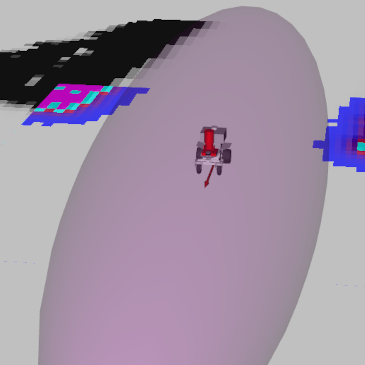
\includegraphics[width=0.75\textwidth]{img/GNSS_cov_high.png}
        \caption{\textsc{High Uncertainty in One Direction}}
        \label{fig:high_uncertainty}
    \end{subfigure}
\caption{\textsc{Standard Deviations and Uncertainty}}
\label{fig:uncertainty_shape}
\end{figure}
\noindent
Nevertheless, in both cases shown in fig. \ref{fig:uncertainty_shape}, the standard deviations are in the meter range, which is not optimal. With RTK available, the deviations,
i.e., the violet shape, should be much smaller in the centimeter or even millimeter range. It is of some importance to detect and report changes in position accuracy.\newline
The monitoring for GNSS failures works as follows. First, there is a qualitative assessment of GNSS links that work in principle based on the information in the \code{NavSatFix}
message. If the connection is not perfect, the mission is not immediately interrupted, but it is at least documented.
The quality is rated as high, if the status is \code{STATUS_GBAS_FIX}, i.e., with ground-based augmentation such as RTK, the covariance type is $\geq$ 
\code{COVARIANCE_TYPE_DIAGONAL_KNOWN} (diagonal known or entirely known), and each standard deviation satisfies a user-defined upper bound $d_{max} \in \mathbb{R}_{0}^{+}$,
i.e., $\sqrt{c_{ii}} \leq d_{max} \thinspace \forall \thinspace i \in \{E, N, U\}$. The last entry of the matrix, i.e., $c_{UU} \in C$ , may not always be present, so
$c_{UU} \in \mathbb{R}_{0}^{+} \cup \emptyset$. It is classified as tolerable if the status is $\geq$ \code{STATUS_FIX}, the covariance type is $\geq$
\code{COVARIANCE_TYPE_APPROXIMATED}, and the standard deviations in turn satisfy $d_{max}$. 
Finally, it is classified as low if it provides a position belief state ($\geq$ \code{STATUS_FIX}), but the covariance
type is unknown. So much for the qualitative assessment of a GNSS link that works in principle.\newline
The first type of monitoring for real failures that interrupt \code{NORMAL_OPERATION} is the status monitoring.
If the status is not set to one of the available options (\code{STATUS_NO_FIX}, \code{STATUS_FIX},
\code{STATUS_SBAS_FIX}, \code{STATUS_GBAS_FIX}), a contingency is initiated, i.e., a message on \code{/contingency_preemption} interrupts the normal operation.
Furthermore, if the status is \code{STATUS_NO_FIX}, the GNSS system was unable to find the position, which is certainly a problem for localization that causes a contingency
case. Status monitoring also checks for cases of \code{STATUS_FIX}, which means that pure GNSS was used for positioning and no RTK is available. However, this is not a reason for
contingency, just information worth publishing on \code{/robot_info}. What is also worth reporting, but does not trigger a contingency, is an unknown service, i.e., when the
\code{NavSatFix} message does not contain any of the available GNSS services \textit{GPS}, \textit{GLONASS}, \textit{Compass} or \textit{Galileo}. Again more critical is the latitude ($lat$) / longitude ($lng$) belief state
monitoring. It is ensured that both values are present and satisfy their respective domains, i.e., $lat \in [-90\degree, 90\degree]$ and $lng \in [-180\degree, 180\degree]$. Altitude is not taken into account
because many GNSS receivers do not provide this information.\newline

\noindent
Eventually, there is uncertainty assessment, i.e., covariance monitoring. 
First, it is checked whether the covariance type corresponds to one of the
available options (\code{UNKNOWN}, \code{APPROXIMATED}, \code{DIAGONAL_KNOWN}, \code{KNOWN}). Otherwise,
a notification is sent to the operator, but of course not a contingency, as this is not critical. The most meaningful components of the covariance matrix are the variances or, more
precisely, the standard deviations, i.e., the square root of the diagonal values, because they actually provide information about the accuracy of the estimated position.
As for the actual standard deviation values, two things can be observed: The absolute values (appropriate / too high) and their progression over time.
The latter is implemented as a variance history in the form of a fixed-length list that always stores the diagonals of the last $n \in \mathbb{N}$
covariance matrices and performs a list shift in which the oldest one is removed when a new one arrives. The length $n$ is again configurable by the user. In the analysis of the variance
history, the square roots, i.e., the standard deviations, are considered, since, as mentioned, these are the crucial values provided by many GNSS receivers.
Whenever the covariance type of an incoming \code{NavSatFix} message is $\geq$ \code{COVARIANCE_TYPE_DIAGONAL_KNOWN}, the history is updated. On the arrival of new feasible 
messages, the deviation progression is analyzed. Such an analysis primarily examines the standard deviations of the east and north components, but also those of the upward component,
if present.\newline
First, it is checked whether the history contains only increasing values for the respective component. If this is the case and, in addition, the difference between the
oldest and the newest deviation is greater than a user-defined significant deviation increase $d_{inc} \in \mathbb{R}_{0}^{+}$, a contingency is initiated. Thus, the definition of
an inappropriate deviation progression is exclusively increasing values combined with an overall absolute increase between the oldest and latest value that exceeds a certain threshold.
Finally, there is one last check, which relates to the absolute values. If the type is $\geq$ \code{COVARIANCE_TYPE_DIAGONAL_KNOWN}, the present variances 
$c_{ii} \in \mathbb{R}_{0}^{+} \thinspace \forall \thinspace i \in \{E, N, U\}$ can with a clear conscience be used for quality assessment. If any of the standard deviations exceeds the user-specified maximum deviation threshold $d_{max}$,
i.e., $\exists \thinspace c_{ii}, i \in \{E, N, U\} : \sqrt{c_{ii}} > d_{max}$, the normal operation is interrupted by publishing to \code{/contingency_preemption}. 
If the type is \code{COVARIANCE_TYPE_APPROXIMATED}, the variances can be considered, but with caution, without giving it too much weight.
The standard deviations $\sqrt{c_{ii}} \in C \thinspace \forall \thinspace i \in \{E, N, U\}$ are checked, but high values exceeding the threshold do not cause a contingency, only a message on \code{/robot_info}.
In principle, it would also be useful to monitor the off-diagonal elements of the covariance matrix, i.e., the actual covariances, since these elements provide information about the
reciprocal relationship of the directions under consideration. For instance, if $c_{NE} < 0$, a negative deviation in the north direction is likely to be matched by a positive deviation in
the east direction, and vice versa. However, in the scope of this work, the monitoring of the covariance matrix will be limited to the above cases.\newline
It is crucial that the approaches
are essentially compatible with all systems using \code{NavSatFix} and are not limited to the AROX system or the present scenario. Hence, for a system to use GNSS monitoring, it simply needs
to publish \code{NavSatFix} messages on \code{/fix}.\newline

\noindent
As before, evaluation of potential problem cases as well as monitoring procedures requires simulation of such cases, which is performed in the \code{GNSS Simulator} described above.
The timeout failure can be easily simulated by unsubscribing the \code{/fix_plugin} topic for a period of time that exceeds the time limit. Quality estimation can be evaluated by
simply configuring the status, covariance information, and service according to the above definition. Monitoring of status, service and position belief state can be simulated by
setting inappropriate values for each. Likewise, absolute deviation monitoring as well as variance history analysis can be tested by simulating the respective problems.
Let the type be \code{COVARIANCE_TYPE_DIAGONAL_KNOWN}, the user-specified history length $n = 4$ and the deviation increase threshold in meters $d_{inc} = 5$. Deviation monitoring
can then be tested by publishing the following (co)variance progression ($n = 4$ messages in sequence):
\begin{figure}[H]
    \begin{subfigure}[b]{0.24\textwidth}
    \centering
        $\left(
        \begin{array}{rrr}
        \boldsymbol{16.2} & 0.0 & 0.0 \\
        0.0 & \boldsymbol{4.4} & 0.0 \\
        0.0 & 0.0 & \boldsymbol{16.5} \\
        \end{array} \right) $
        \caption{\textsc{}}
        \label{fig:oldest}
    \end{subfigure}
    \hfill
    \begin{subfigure}[b]{0.24\textwidth}
    \centering
        $\left(
        \begin{array}{rrr}
        \boldsymbol{25.1} & 0.0 & 0.0 \\
        0.0 & \boldsymbol{9.8} & 0.0 \\
        0.0 & 0.0 & \boldsymbol{16.8} \\
        \end{array} \right) $
        \caption{\textsc{}}
        \label{fig:}
    \end{subfigure}
    \hfill
    \begin{subfigure}[b]{0.24\textwidth}
    \centering
        $\left(
        \begin{array}{rrr}
        \boldsymbol{89.0} & 0.0 & 0.0 \\
        0.0 & \boldsymbol{64.2} & 0.0 \\
        0.0 & 0.0 & \boldsymbol{81.3} \\
        \end{array} \right) $
        \caption{\textsc{}}
        \label{fig:}
    \end{subfigure}
    \hfill
    \begin{subfigure}[b]{0.24\textwidth}
    \centering
        $\left(
        \begin{array}{rrr}
        \boldsymbol{99.4} & 0.0 & 0.0 \\
        0.0 & \boldsymbol{77.7} & 0.0 \\
        0.0 & 0.0 & \boldsymbol{98.3} \\
        \end{array} \right) $
        \caption{\textsc{}}
        \label{fig:latest}
    \end{subfigure}
\caption{\textsc{(Co)variance History (Old to New)}}
\label{fig:cov_history}
\end{figure}
\noindent
The (co)variance progression depicted in fig. \ref{fig:cov_history} is expected to cause a contingency for various reasons, e.g., due to the fact that the history only
contains increasing standard deviation values for the east component ($\sqrt{16.2} m \rightarrow \sqrt{25.1} m \rightarrow \sqrt{89.0} m \rightarrow \sqrt{99.4} m$) and the overall
absolute increase between the east deviation of the oldest (cf. fig. \ref{fig:oldest}) and latest (cf. fig. \ref{fig:latest}) covariance matrices exceeds the defined threshold
of $5 m (\approx 5.95 m)$. It is reasonable to interrupt normal operation in such a case, as such a (co)variance progression poses great challenges for localization.\newline

\noindent
The simulation of the GNSS failure cases can be enabled / disabled via the following ROS topics:
\begin{itemize}
    \item \textbf{disconnect / timeout:} \code{/toggle_simulated_timeout_failure}
    \item \textbf{good quality:} \code{/set_simulated_good_quality}
    \item \textbf{medium quality:} \code{/set_simulated_med_quality}
    \item \textbf{low quality:} \code{/set_simulated_low_quality}
    \item \textbf{unknown status:} \code{/set_simulated_unknown_status}
    \item \textbf{no fix:} \code{/set_simulated_no_fix}
    \item \textbf{no RTK:} \code{/set_simulated_no_rtk}
    \item \textbf{unknown service:} \code{/toggle_simulated_unknown_service}
    \item \textbf{infeasible lat / lng:} \code{/toggle_simulated_infeasible_lat_lng}
    \item \textbf{variance history failure:} \code{/toggle_simulated_variance_history_failure}
    \item \textbf{high deviation:} \code{/toggle_simulated_high_deviation}
\end{itemize}

\subsection{Data Management}
\label{sec:sim_and_mon_data_management}

Similar to sensor monitoring, executing a \code{scan} action launches the data monitoring procedure, which looks for the potential data management issues presented in
section \ref{sec:challenges_for_lta}. To perform the drive capacity check, i.e., to determine whether the drive on which scan logging or data storage in general takes place has enough
free space, the cross-platform library \code{psutil}\footnote{\textcolor{link-color}{\url{https://pypi.org/project/psutil/}}} is used. It provides a function \code{disk_usage()} which returns the load of the
specified disk, e.g., the one configured in \code{MONITOR_DRIVE}. Unlike WiFi connection monitoring, where the actual low-level network connectivity checks are outsourced
from the monitoring framework due to its operating system coupling, disk capacity checks can be part of the framework itself because of the cross-platform nature of \code{psutil}.\newline
If the result of \code{disk_usage(MONITOR_DRIVE)} exceeds $99\%$, the node detects a full memory and causes an interruption of the robot's mission and a transition to the
\code{CONTINGENCY} state. Additionally, notifications are sent to the operator when the disk load exceeds $95\%$ and $90\%$, with an indication that the data should be backed up
externally soon. So much for very general data management monitoring, which in principle can be used for all types of data acquisition tasks, since the type of data is irrelevant
to capacity testing. There is also a more scenario-specific part based on certain assumptions and dependencies that is optional and can be enabled or disabled by the user.
This is the specific scan logging monitoring that assumes that the data acquisition task at hand is a scanning task, such as the one described in section
\ref{sec:lta_plant_observation}, and that the scans are written to a user-configured directory by the dummy scanning node described in section
\ref{sec:dummy_scanning_node}. Since the data format of the scans written by the dummy scanner is well-known, i.e., \code{LaserScan} or \code{PointCloud2}, the entries logged in
this log file can be easily evaluated. The idea is that there should be an additional scan entry in the log file after a successful scan action. If that is not the case,
a data management error has been detected and a transition to \code{CONTINGENCY} is initiated. It would also be possible to implement some sort of exception escalation system
based on sensor logging errors, but since this would require in-depth knowledge of implementation details of the sensors used, it was renounced.\newline
General capacity monitoring is based on the idea of not having dependencies on specific scenarios or configurations, and instead just monitor the configured path and communicate
when certain thresholds are exceeded, which, as mentioned, basically works for any data acquisition task. However, the goal of ensuring a certain level of generality applies to
both cases. Of course, the second case is only suitable for laser scanning tasks, but it is not limited to one specific sensor. It can deal with all kinds of sensors that provide
results in the form of \code{LaserScan} or \code{PointCloud2}, which covers quite some generality. Therefore, a specific sensor such as the \textit{RIEGL} (cf. fig.
\ref{fig:arox_system}) can be replaced by another model without any problems, and data monitoring should continue to work based on the slight constraint of producing data of the
two mentioned types. General capacity monitoring works either way. Since the logging of the data always follows the scanning and the scanner is the module that writes the scans to
the file system, it would be superfluous to check the data again for plausibility, as this is already part of the sensor monitoring. It suffices to verify whether the storing
operation, i.e., writing the scan to the log file, worked. Moreover, it is worth noting that a total sensor failure always implies a data management failure of the second type,
but this should already be detected by the sensor monitoring procedure. Of course, more checks could be made for scenario-specific logs on the drive, etc., but since this would
require additional knowledge of the specific circumstances, it would violate the goal of being as general as possible. Nevertheless, it is possible to extend data management in
the future to include application-specific monitoring aspects that can be easily disabled to maintain general applicability. For a system to use the data management monitoring node,
it must indicate scan actions via \code{/scan_action} and their completion via \code{/scan_completed}. Furthermore, \code{MONITOR_DRIVE} as well as \code{SCAN_PATH} need to be
configured.\newline

\noindent
It is not a big challenge to simulate the occurrence of the data management problems presented in section \ref{sec:challenges_for_lta}. To simulate a \textquote{full disk}-failure,
i.e., a full memory of the drive on which the scans are to be logged, one could simply prepare a full USB flash drive and configure the path to be monitored accordingly,
e.g., mount the flash drive to \code{/mnt/usb} and set \code{MONITOR_DRIVE = /mnt/usb}. It is also implemented in such a way that one can simply prepare the flash drive and later publish
to \code{/sim_full_disk_failure}, which will then set the \code{MONITOR_DRIVE} to \code{/mnt/usb}. The second and more scenario-specific type of error is the scan logging error,
which can be simulated by simply not writing the scan to the file system in the dummy scanning node introduced in section \ref{sec:dummy_scanning_node}. Simulation of this type
of error can be enabled / disabled via the ROS topic \code{/toggle_simulated_scan_logging_failure}. Data management issues can be addressed with the resolution methods described
in section \ref{sec:data_management_resolver}.

\subsection{Plan Deployment Failure}
\label{sec:sim_and_mon_plan_deployment_failures}

There are several potential failures regarding the deployment of generated plans. The first and most apparent is a missing plan, i.e., a situation where the robot is ready in
principle to perform a mission, but no plan arrives and it remains in the \code{IDLE} state. Since this is not an error per se and this case may be perfectly valid, once a certain
threshold is exceeded, it merely triggers a notification via \code{/robot_info} to the human operator and keeps notifying at a specified frequency. The information whether a plan
has been received, i.e., a mission is being executed, is retrieved via a configurable topic, in the scenario described in section \ref{sec:prototype_scenario} via
\code{/arox/ongoing_operation}. Additionally, the \code{PlanDeploymentMonitor} subscribes to a topic \code{/plan_retrieval_failure} on which the embedded low-level operation state
machine publishes as its normal error treatment behavior in case of plan retrieval failures, e.g., exceptions. There are defined error codes published on this topic ($0$: plan
retrieval service unavailable, $1$: empty plan, $2$: infeasible plan). Based on this error code, the \code{PlanDeploymentMonitor} initiates a contingency with an appropriate message
explaining the reason, using the \code{/contingency_preemption} topic. Monitoring of plan deployment failures is
therefore a special case, since most of the monitoring is based on error handling reported by the operational state machine. However, this makes sense because these errors are
naturally detected in the operation state machine and only need to be reported or passed on to the higher-level state machine for execution monitoring. Brodskiy et al. refer to these
types of failures recognized and indicated within a component as \textit{signaled failures} and argue that it is desirable to cover as many aspects as possible by such signaled
failures, with each component being more or less self-responsible. \cite{Brodskiy:2011}\newline

\noindent
The exact error treatment responsible for detecting these errors works as follows. First, the plan generation node described in section \ref{sec:plan_generation} provides plans via the
\code{arox_planner/get_plan} service. If a call to this service triggers a timeout exception, it gets caught, the error is reported (code $0$), and the operation state machine
remains in the \code{IDLE} state. Analogously, a plan with an empty list of actions (code $1$) and a plan containing an action of an unknown type (code $2$) is recognized and
reported. The detection of actions of an unknown type is based on a configurable list of actions that are expected, e.g., \code{drive_to}, \code{return_to_base}, \code{charge}
and \code{scan} in the considered scenario. In order to allow the monitoring node to initiate the contingency without the operational state machine immediately transitioning back
to \code{IDLE} and repeatedly requesting a plan, a short delay (e.g. $1s$) is introduced for each detected problem to avoid unnecessary timing conflicts during transitions.
Thus, in order for other systems to be able to use the plan deployment monitoring, the mentioned topics and the action list must be configured. Moreover, explicit errors can be
communicated via \code{/plan_retrieval_failure} using the described error codes.\newline

\noindent
For simulation, it is quite obvious that it is reasonable to simulate the failures where they occur, i.e., in the plan generator (cf. section \ref{sec:plan_generation}). The
situation of an extended idle time is simulated by simply blocking the plan fetch for a configurable period of time, which must be greater than or equal to the threshold defined
in \code{PlanDeploymentMonitor}. The simulation of an unavailable plan service is done by temporarily shutting down the service using the \code{shutdown} method provided by ROS services.
Empty and otherwise infeasible plans are trivially simulated by either clearing the list of actions or setting one of the action names to an unspecified string.
The simulation of the plan deployment failure cases can be enabled via the following ROS topics:
\begin{itemize}
    \item \textbf{extended idle time:} \code{/sim_extended_idle_time}
    \item \textbf{unavailable plan service:} \code{/toggle_unavailable_plan_service}
    \item \textbf{empty plan:} \code{/sim_empty_plan}
    \item \textbf{infeasible plan:} \code{/sim_infeasible_plan}
\end{itemize}
\noindent
Plan-deployment-related challenges for LTA can be addressed using the resolver described in section \ref{sec:plan_deployment_resolver}.

\subsection{Navigation Failure}
\label{sec:sim_and_mon_navigation_failures}

Since the identified challenges of \textit{Obstacles Blocking the Planned Path} and \textit{Sustained Recovery} (cf. sec. \ref{sec:challenges_for_lta}) are also essentially navigation problems, the three challenges are
considered together under the heading \textit{Navigation Failure}. Although sustained recoveries could in principle refer to all kinds of problems, this thesis is limited to
sustained recoveries in the case of navigation problems, as this is by far the most relevant case from a practical perspective. Thus, it is sustained recoveries induced by
\code{move_base_flex}.\newline

\noindent
Recovery behaviors should naturally vary between static and dynamic obstacles. A dynamic obstacle like a person or an animal will in most cases simply walk through the scene and
disappear a moment later, so waiting for a moment can already be a very reasonable and sufficient recovery behavior. Static obstacles, on the other hand, may be present for longer
periods of time, requiring more sophisticated recovery behaviors. \code{move_base_flex} is generally already able to detect obstacles. The task of a monitoring procedure in this
case is to closely observe what \code{move_base_flex} is doing and intervene if necessary. Concerning the obstacles, there are two distinct cases: Either the obstacles only block
the direct path, but there is still one, or the obstacles actually block every single path and the robot cannot reach its destination. In the first case, it would be preferable if
the robot was able to find it, but if it is incapable of doing so, it should be detected and communicated. This is basically the case of navigation failures in the sense that there
is a path to the navigation goal, but \code{move_base_flex} cannot find it (cf. fig. \ref{fig:nav_fail}). Fig. \ref{fig:nav_fail} shows a side by side comparison of what the robot
perceives and the actual section of the simulated world. In fig. \ref{fig:nav_fail_rviz}, the route currently considered by \code{move_base_flex} (green line) as well as the target
pose (cyan arrow) is depicted. Examining the actual world excerpt in fig. \ref{fig:nav_fail_gazebo}, it is obvious that this route will not lead the robot to its destination. However, as
can be observed from fig. \ref{fig:nav_fail_gazebo}, there is a viable route (red line) that would accomplish this. Fig. \ref{fig:nav_fail_rviz} shows how the local
planner (\textit{EBand}) tries to satisfy a global plan that is faulty due to lack of information. The local route that the robot takes in fig. \ref{fig:nav_fail_rviz} does not
lead to the correct global one indicated in fig. \ref{fig:nav_fail_gazebo}. In some cases, \code{move_base_flex} may find the viable route after a while,
but this is not assured. The problem in such cases is often that the viable routes are somehow counterintuitive, e.g., because they require a detour, at least given the robot's partial
knowledge of the environment. Analogous to leaving local optima in optimization, in some circumstances the robot must first navigate farther away from the target before it can actually
reach it.

\vfill
\pagebreak

\begin{figure}[H]
    \centering
    \begin{subfigure}[b]{0.49\textwidth}
        \centering
        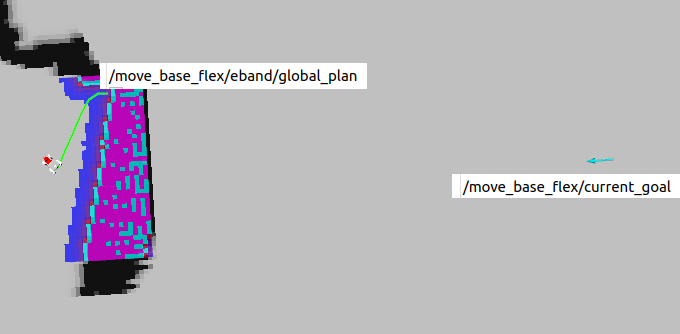
\includegraphics[width=\textwidth]{img/nav_fail_wrong_route_0.png}
        \caption{\textsc{Considered Route (rviz\footnotemark)}}
        \label{fig:nav_fail_rviz}
    \end{subfigure}
    \hfill
    \begin{subfigure}[b]{0.49\textwidth}
        \centering
        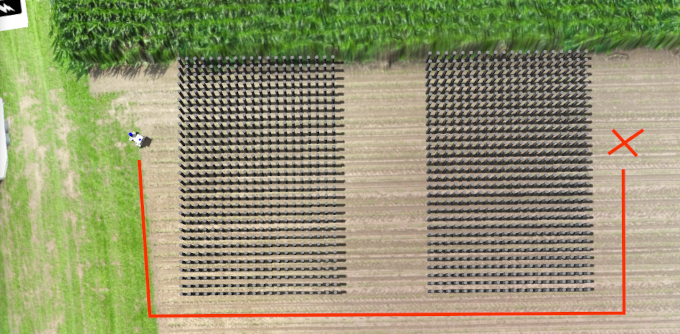
\includegraphics[width=\textwidth]{img/nav_fail_wrong_route_1.png}
        \caption{\textsc{Feasible Route (Gazebo)}}
        \label{fig:nav_fail_gazebo}
    \end{subfigure}
\caption{\textsc{Navigation Failure - Unable to Find a Path to the Goal}}
\label{fig:nav_fail}
\end{figure}
\footnotetext{$3D$ Visualization Tool for ROS (\textcolor{link-color}{\url{https://wiki.ros.org/rviz}})}
\noindent
This example is by no means contrived, it is not unrealistic that in practice the robot is regularly confronted with such situations, meaning that it is important to recognize them
and enable the system to cope with them. To give an example from the scenario under consideration: An unexpected obstacle could block the path of the robot, e.g., a large agricultural machine. 
If the local costmap, which is usually between $3 \times 3$ and $5 \times 5$ meters, is smaller than the obstacle, this problem arises. The keyword here is \textit{sensor horizon},
if it is too small, it can lead to problems like this. On the other hand, it should be as small as possible to save runtime and increase efficiency. In general, the problem arises
from the fact that \code{move_base} and \code{move_base_flex} work with two layers, i.e., two maps, the global map where everything is static and known, and the local map for dynamic
obstacles, which is initially empty. Now back to the example of the agricultural machine blocking the robot's path. Since this machine is not a static object that is part of the
global map, it can only be recognized as part of the local map. However, the local costmap shows a section of the machine that is at most as large as the local costmap. Moreover,
everything that leaves the local costmap is \textquote{forgotten} by the robot. This leads to absurd situations in which the robot drives along the obstacle and forgets about it when
parts of it leave the sensor horizon, so that the path behind it appears clear again. Thus, the robot oscillates back and forth in an endless loop. A simple remedy, which is not
a panacea but is practically used in the considered scenario, is to simply copy information from the local map to the global map so that the local obstacles can be taken into
account in the global planning (\code{move_base_flex}). This assumes that everything the robot perceives locally is transferred to the static global costmap so that it is henceforth
considered static. This approach misuses the global static map as a knowledge base for local sensor information. Yet, not persistently, but only as working memory, only during
the runtime of the robot. An obvious problem is that this assumption does not hold, since in this approach dynamic obstacles such as people can be erroneously entered into the global
map and henceforth be considered static obstacles. This happens when a person remains stationary until leaving the sensor horizon of the robot. Nevertheless, since such cases are much
rarer compared to the first issue, this workaround proved to be practically useful in this particular context. In the long term, of course, a more sensible solution must be developed.\newline

\noindent
So much for situations that can be solved in principle. In the other case (obstacles block every single path), however, it should be detected and communicated in any case, because the robot can not solve it itself. If the robot is unable to successfully generate a
path, there are essentially two different outcomes, regardless of whether this is because there is no path or because it simply cannot find it. First, it results in a sustained
recovery. Second, it simply fails with an error and aborts the navigation target. Both cases should be recognized. During practical experiments in this work, there were many
situations where \code{move_base_flex} was unable to find a correct path and simply ended up in a loop of failed recoveries without ever returning to normal operation. In this
case, the robot should try a few different recovery actions and then abort and report the problem. Monitoring methods must therefore track the results / states of recovery
behaviors and decide whether it is appropriate to try more or stop. To identify sustained recovery situations, it is necessary to count them somehow. \code{move_base_flex}
communicates its status via the ROS topic \code{/move_base_flex/exe_path/status}. Consequently, to count the number of failed recoveries, one can simply count the transitions
from \code{GoalStatus.ACTIVE} to \code{GoalStatus.ABORTED}. \code{GoalStatus.SUCCEEDED} should always reset the counter, because then the recovery has actually solved the problem.\newline

\noindent
Monitoring is performed at a frequency specified by the user and verifies the current recovery count $r \in \mathbb{N}$. Whenever $r = 1$, i.e., when the first recovery occurs after successful
operation, the current position of the robot is stored using the GNSS data obtained from the \code{/fix} topic (cf. section \ref{sec:sim_and_mon_gnss_connection_problems}). If the
recovery count reaches a user-configurable recovery limit $l \in \mathbb{N}$, i.e., $r \geq l$, a contingency is initiated via \code{/contingency_preemption} due to a sustained recovery. This method covers a sustained recovery, as it
arises from a case of obstacles without the possibility of circumvention. Combined with a check for explicit \code{move_base_flex} errors, this covers all expected navigation failures, since
they will all end with a persistent recovery or an explicit termination. The explicit check works as follows. The navigation monitoring node maintains a subscription to
\code{/explicit_nav_failure} through which external procedures, such as the low-level operation state machine, can trigger a contingency due to a navigation problem. For this
purpose, the operation state machine publishes to \code{/explicit_nav_failure} and notifies the monitoring procedure whenever a navigation goal issued to
\code{move_base_flex} explicitly returns \code{GoalStatus.ABORTED}. This is again an example of \textit{signaled failures} proposed by Brodskiy et al. \cite{Brodskiy:2011} and
discussed earlier in section \ref{sec:sim_and_mon_plan_deployment_failures}.\newline

\noindent
One problem is that repeated recoveries in which some progress is actually achieved should not be mistaken as
sustained recoveries and thus failure. Hence, one should not only count the repetitions and declare that it has failed after a number of unsuccessful attempts, i.e., $r \geq l$, but
also take into account reasonable progress towards the goal. For instance, if the robot approaches the target during the process rather than just rotating on the spot, it should be
viable. For this purpose, each time when $r \geq l$, a further check is performed before a contingency is triggered, namely comparing the stored position of the robot at the beginning of
the recovery sequence with the present position. If the distance between the two locations is less than a user-configurable lower bound, the robot has not made sufficient progress
and a contingency is initiated. Otherwise, the robot has performed a number of recoveries, but with some success as it progresses towards the goal, so this is not considered a
failure. In such cases, the operator is informed via \code{/robot_info}, the recovery counter is reset, i.e., $r = 1$, the initial recovery position is set to the present position
and the recovery process can be continued.\newline

\noindent
It is important to note that monitoring is kept as generic as possible to be compatible with other scenarios and applications involving autonomous mobile robots.
For instance, it is easy to switch to the common navigation framework \code{move_base} by simply changing the topic configuration.
The counting of transitions etc. should still work, because \code{move_base} works with the same \code{GoalStatus} information.
Essentially, any navigation framework that is compatible with the general \code{actionlib_msgs/GoalStatus}\footnote{\textcolor{link-color}{\url{https://docs.ros.org/en/lunar/api/actionlib_msgs/html/msg/GoalStatus.html}}} is compatible with the introduced monitoring solution.
For a system to use the navigation monitoring node, it simply needs to specify the \code{GOAL_STATUS_TOPIC} under which the \code{GoalStatusArray}\footnote{\textcolor{link-color}{\url{https://docs.ros.org/en/lunar/api/actionlib_msgs/html/msg/GoalStatusArray.html}}} messages appear. Additionally,
\code{NavSatFix} messages are again expected to appear on \code{/fix} to track progress in cases of sustained recovery. As described, the topic \code{/explicit_nav_failure} can be
used to report explicit navigation errors. Of course, it would be possible to simply extend the \code{move_base_flex} state machine to perform this type of monitoring, but doing so
would only solve the problem for a specific framework, which would contradict the claim of achieving some generality.\newline

\noindent
Sustained recoveries as well as explicit \code{move_base_flex} failures can be evaluated in simulation by inducing situations where recovery is not possible, e.g., when the
path to the destination is blocked and there is no other way, i.e., by specially constructed examples that are particularly difficult for the navigation algorithms to solve.
The occurrence of static and dynamic obstacles can be implemented in the simulation by spawning mobile and immobile objects at randomized positions that could potentially block
the robot's path. However, as mentioned earlier, dynamic obstacles are generally not a major concern as they will appear as obstacles, initiate a recovery, usually a turn on the
spot, and after that, in most cases, the obstacle has already disappeared and the robot can continue its mission. If this is not the case, it could be treated as static anyway.
Therefore, only the harder case of unexpected static obstacles is considered here, since this is the case to which the robot actually has to adapt.\newline
The most extreme case of an
unexpected static obstacle would be one that blocks all paths between the robot and its navigation target, so that it simply cannot reach it. In order to simulate certain scenarios
with obstacles systematically, the \code{ObstacleSpawner} was developed. The obstacle models used must be stored in \code{home/.gazebo/models} and are all freely available
\footnote{\textcolor{link-color}{\url{http://models.gazebosim.org/}}}. The ROS service \code{/gazebo/spawn_sdf_model} is used to spawn the obstacle models. The service must be called with the model name,
the XML model read from file, an initial pose and a reference frame. The extreme case is simulated by spawning a \textquote{robot prison} (cf. fig. \ref{fig:robot_prison}). Any
navigation target outside the prison leads to an error situation, which should be recognized. The idea is to dynamically spawn obstacles around the robot's current location, encircling
it. Since this is only a simulation, the $x$ and $y$ coordinates of the robot's current world position ($r_x, r_y$) can be taken from the \code{/pose_ground_truth} topic.
As the ground truth provides the orientation as quaternion, the $z$ orientation, i.e., the yaw angle $r_\psi$ is computed using \code{tf.transformations.euler_from_quaternion}.
Now the idea is to spawn the four barriers depicted in fig. \ref{fig:robot_prison}. Therefore, the poses of all four barriers have to be computed relative to the robot's current
pose. The barrier height $b_h \in \mathbb{R}$ and the distance $b_d \in \mathbb{R}$ to the robot are the same for all four and configurable by the user. In addition, the roll $\phi$
and pitch $\theta$ angles are always $0$. More interesting are the $x$ and $y$ coordinates as well as the yaw angle $\psi$ of each barrier, which are computed as follows:
\begin{itemize}
    \item \textbf{barrier right:} $\boldsymbol{b_x^r} \coloneqq r_x + (b_d \cdot \cos{(\frac{\pi}{2} + \psi})), \thinspace \boldsymbol{b_y^r} \coloneqq r_y + (b_d \cdot \sin{(\frac{\pi}{2} + \psi)}), \thinspace \boldsymbol{b_\psi^r} \coloneqq r_\psi$
    \item \textbf{barrier left:} $\boldsymbol{b_x^l} \coloneqq r_x + (b_d \cdot \cos{(1.5 \pi + \psi})), \thinspace \boldsymbol{b_y^l} \coloneqq r_y + (b_d \cdot \sin{(1.5 \pi + \psi)}), \thinspace \boldsymbol{b_\psi^l} \coloneqq r_\psi$
    \item \textbf{barrier front:} $\boldsymbol{b_x^f} \coloneqq r_x + (b_d \cdot \cos{(\psi})), \thinspace \boldsymbol{b_y^f} \coloneqq r_y + (b_d \cdot \sin{(\psi)}), \thinspace \boldsymbol{b_\psi^f} \coloneqq r_\psi + \frac{\pi}{2}$
    \item \textbf{barrier back:} $\boldsymbol{b_x^b} \coloneqq r_x + (b_d \cdot \cos{(\pi + \psi})), \thinspace \boldsymbol{b_y^b} \coloneqq r_y + (b_d \cdot \sin{(\pi + \psi)}), \thinspace \boldsymbol{b_\psi^b} \coloneqq r_\psi + \frac{\pi}{2}$
\end{itemize}
Thus, the pose passed to the \code{/gazebo/spawn_sdf_model} service proxy to spawn the barrier to the right side of the robot would be $(b_x^r, b_y^r, b_h, 0, 0, b_\psi^r)$.
Since spawning the \textquote{robot prison} takes a moment, it is advisable to do this only when the robot is standing still, otherwise unwanted side effects such as collisions may
occur. Consequently, when the simulation is launched, it will only be executed when the robot is next at a standstill, i.e., when it is in a state other than \code{GoalStatus.ACTIVE}
based on \code{/move_base_flex/exe_path/status}. The \textquote{robot prison} exemplifies cases that cannot be solved by the robot and that should be detected by monitoring.
\begin{figure}[H]
    \centering
    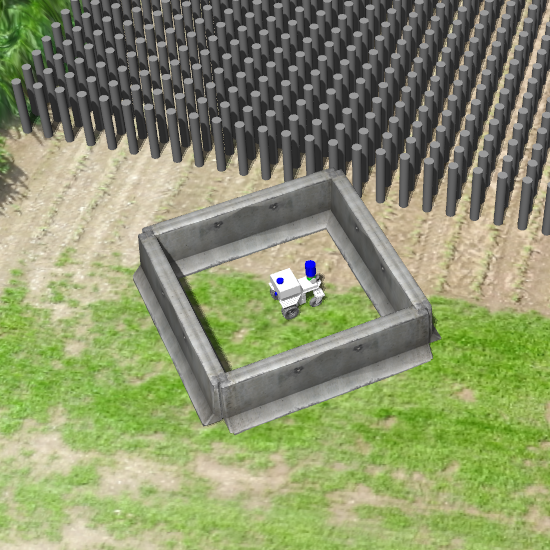
\includegraphics[width=0.45\textwidth]{img/robot_prison.png}
    \caption{\textsc{\textquote{Robot Prison} - Static Obstacles that Completely Confine the Robot}}
    \label{fig:robot_prison}
\end{figure}
\noindent
Furthermore, the following (cf. fig. \ref{fig:obstacle_scenarios}) solvable static obstacle scenarios were implemented in order to test the robot's ability to overcome them. All of
these scenarios are predefined in the \code{ObstacleSpawner} configuration and can be arbitrarily spawned during a robot operation using the \code{/gazebo/spawn_sdf_model} service.
The number plate on the ground always indicates
the target position of the robot in the manual evaluation of the corresponding scenario. However, they also coincide with the general direction in which the robot must overcome them in
a simulated mission, i.e., the prototype scenario described in section \ref{sec:prototype_scenario}. The idea is essentially to block the robot's direct path and see whether it is
able to come up with an alternative. In this manner, the situation that a static obstacle appears on the robot's route can be simulated, and the robot is usually able to manage it.
\begin{figure}[H]
    \centering
    \begin{subfigure}[b]{0.24\textwidth}
        \centering
        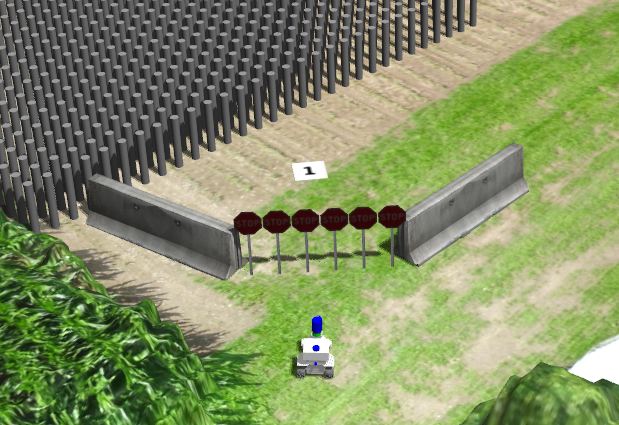
\includegraphics[width=\textwidth]{img/static_1.png}
        \caption{\textsc{Scenario One}}
        \label{fig:static_1}
    \end{subfigure}
    \hfill
    \begin{subfigure}[b]{0.24\textwidth}
        \centering
        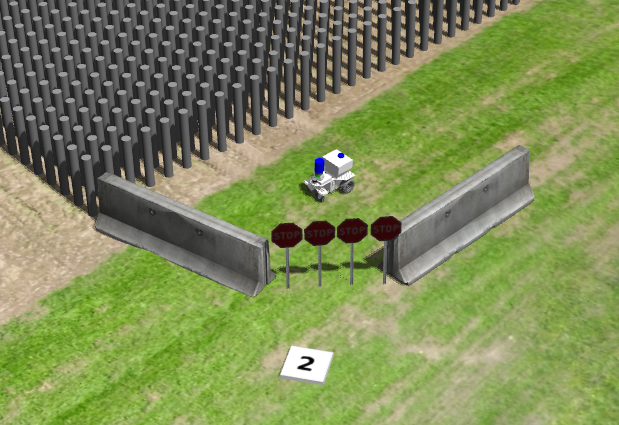
\includegraphics[width=\textwidth]{img/static_2.png}
        \caption{\textsc{Scenario Two}}
        \label{fig:static_2}
    \end{subfigure}
    \begin{subfigure}[b]{0.24\textwidth}
        \centering
        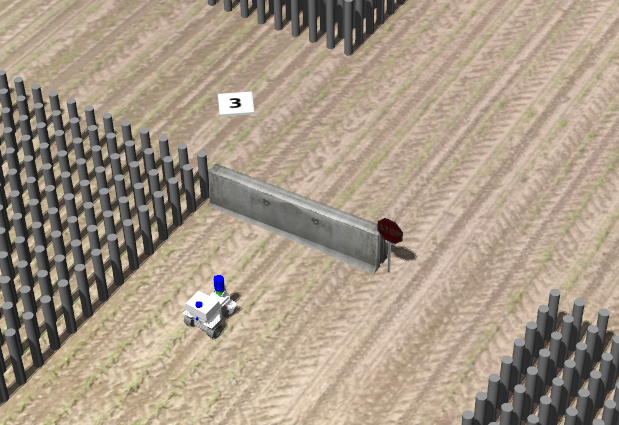
\includegraphics[width=\textwidth]{img/static_3.png}
        \caption{\textsc{Scenario Three}}
        \label{fig:static_3}
    \end{subfigure}
    \hfill
    \begin{subfigure}[b]{0.24\textwidth}
        \centering
        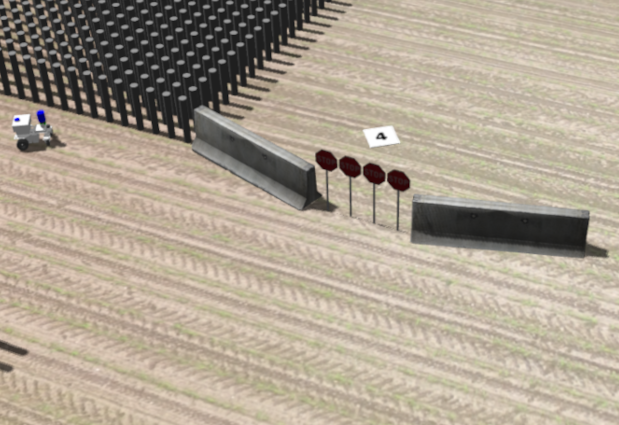
\includegraphics[width=\textwidth]{img/static_4.png}
        \caption{\textsc{Scenario Four}}
        \label{fig:static_4}
    \end{subfigure}
\caption{\textsc{Solvable Static Obstacle Scenarios}}
\label{fig:obstacle_scenarios}
\end{figure}
\noindent
For instance, fig. \ref{fig:obstacle_success} shows how the robot copes with the first scenario (cf. fig. \ref{fig:static_1}). As can be seen, the robot manages to iteratively
progress around the static obstacle until it reaches the blocked target. This illustrates that unexpectedly appearing obstacles are not a great problem as long as there is a way.
Nevertheless, if they are, it will be detected by the aforementioned monitoring method.
\begin{figure}[H]
    \centering
    \begin{subfigure}[b]{0.24\textwidth}
        \centering
        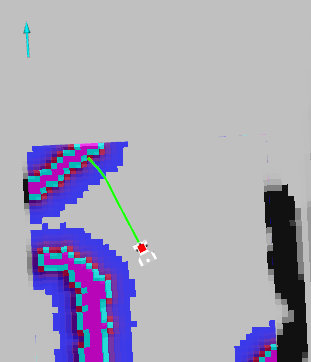
\includegraphics[width=\textwidth]{img/succ_1.png}
        \caption{\textsc{}}
        \label{fig:succ_1}
    \end{subfigure}
    \hfill
    \begin{subfigure}[b]{0.24\textwidth}
        \centering
        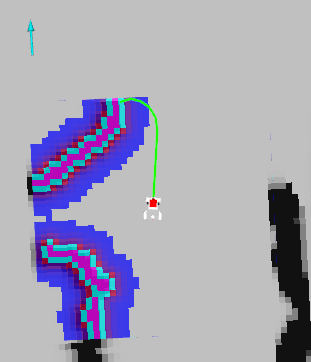
\includegraphics[width=\textwidth]{img/succ_2.png}
        \caption{\textsc{}}
        \label{fig:succ_2}
    \end{subfigure}
    \begin{subfigure}[b]{0.24\textwidth}
        \centering
        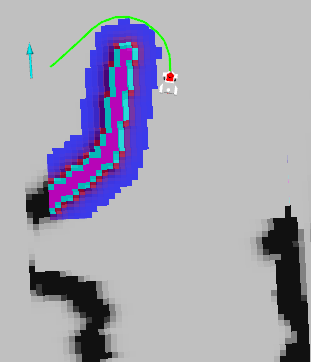
\includegraphics[width=\textwidth]{img/succ_3.png}
        \caption{\textsc{}}
        \label{fig:succ_3}
    \end{subfigure}
    \hfill
    \begin{subfigure}[b]{0.24\textwidth}
        \centering
        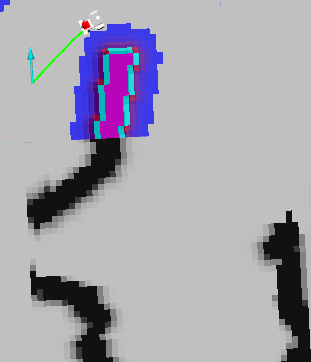
\includegraphics[width=\textwidth]{img/succ_4.png}
        \caption{\textsc{}}
        \label{fig:succ_4}
    \end{subfigure}
\caption{\textsc{Successful Overcoming of Static Obstacle Scenario One}}
\label{fig:obstacle_success}
\end{figure}
\noindent
Unfortunately, it is not trivial to
simulate a case where \code{move_base_flex} fails on every attempt, although there is a path. Depending on the location and surroundings of the robot, it is sometimes able to find
the right way after a while. Yet, it is sufficient to show that such situations exist, as this is adequate justification for the need to address them. The straightforward approach to
simulate such situations works as follows. The user can specify a set of points, e.g., the one (red crosses) shown in fig. \ref{fig:outlier_points} in the scenario described in section \ref{sec:prototype_scenario}.
These points are not hard to reach per se, but should be quite difficult to reach from certain locations, e.g., because there are many obstacles in between.
When simulating such a situation, the point from the specified set of points farthest from the robot's current position is chosen, which does not guarantee navigation problems,
but is a fairly good heuristic. As the user is supposed to specify these points in latitude and longitude, the robot's position is taken from the GNSS estimate, i.e., \code{/fix}.
\begin{figure}[H]
    \centering
    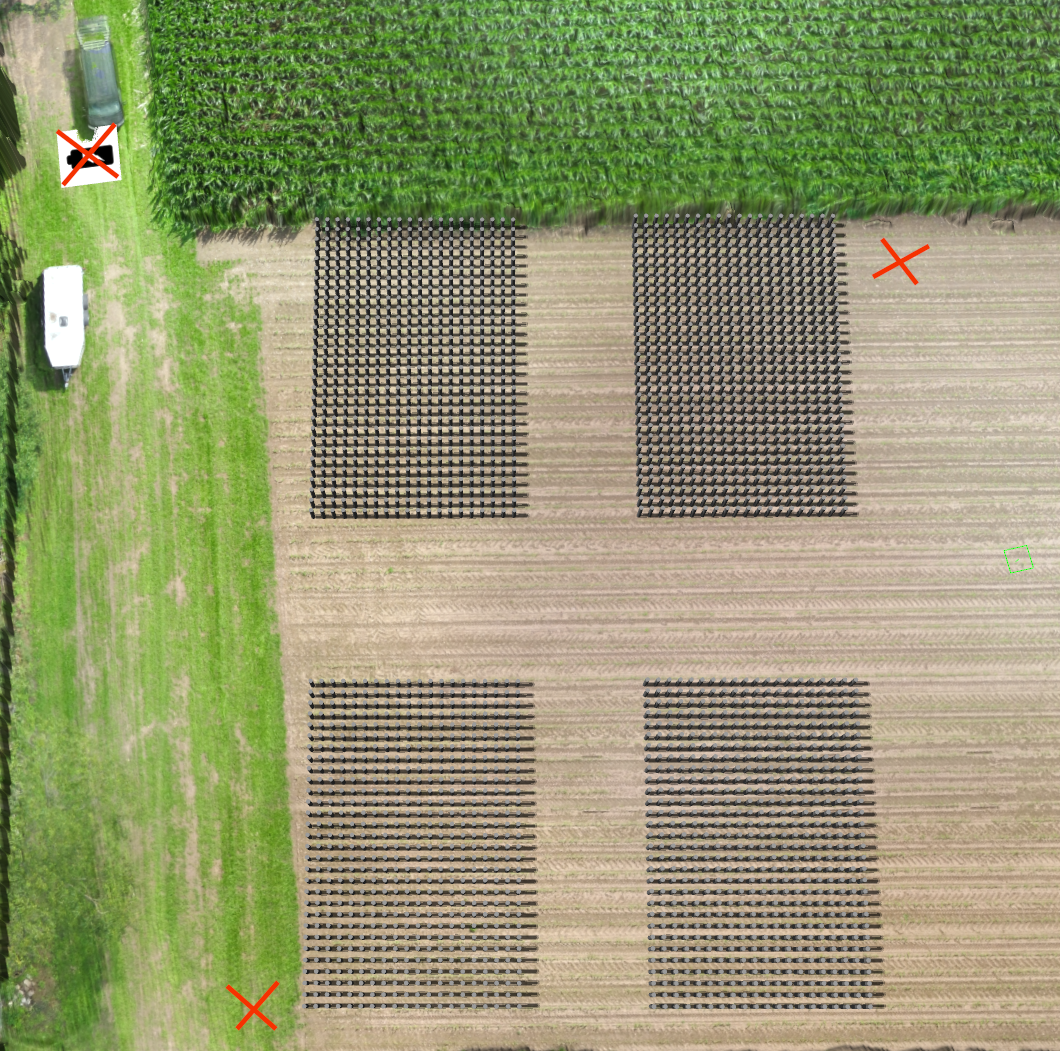
\includegraphics[width=0.35\textwidth]{img/hard_to_reach.png}
    \caption{\textsc{Specified Set of \textquote{Hard-to-Reach} Points in the Prototype Scenario}}
    \label{fig:outlier_points}
\end{figure}
\noindent
As anticipated, this is not a guarantee of navigation failure, but it does cause it on a regular basis (cf. fig. \ref{fig:nav_fail}). It would be infeasible to simply interrupt the
active plan and set the selected point as navigation target, as there would then be no successful outcome that continues the plan. Thus, the dummy target is introduced as an
intermediate action in the plan, an option that is implemented as part of the low-level operation state machine. The \code{ObstacleSpawner} publishes the point to be used on
\code{/introduce_intermediate_nav_goal}, and the operation state machine executes it after the currently active action has been completed.
The simulation of the navigation failures can be enabled via the following ROS topics:
\begin{itemize}
    \item \textbf{static obstacles:} \code{/spawn_static_obstacles} (\code{str msg "scene_n"}, $n \in \{1, 2, 3, 4\}$)
    \item \textbf{robot prison:} \code{/spawn_robot_prison}
    \item \textbf{navigation failure (counterintuitive route):} \code{/trigger_nav_fail}
\end{itemize}
Navigation failures that are in principle solvable, i.e., not inescapable, can be addressed with the resolver described in section \ref{sec:nav_fail_resolver}.

\subsection{Incorrect or Inaccurate Localization}
\label{sec:sim_and_mon_incorrect_localization}

In general, localization is a complex topic whose detailed consideration is far beyond the scope of this work.
Nevertheless, it would be very valuable to develop a monitoring approach that is capable of realizing situations in which the localization is no
longer accurate, as there is a simple workaround that alleviates the problem in practice in many cases: Just driving the robot
a few meters back and forth to recalibrate the localization using different GNSS positions. The localization of the AROX system
is based on three components: IMU (inertial measurement unit), odometry and GNSS. Hence, incorrect or inaccurate localization can only be the product of problems in the pose
estimation of one or more of these components. There are numerous causes of drift and accumulated sensor errors, such as wheel slippage or being exposed to local magnetic fields
or magnetic materials. \cite{Bechar:2016} An implementation of a generalized
extended Kalman filter (cf. ROS community package \code{robot_localization}\footnote{\textcolor{link-color}{\url{https://wiki.ros.org/robot_localization}}}) is used to fuse the data from the different
sensors. The idea of a localization monitoring procedure is to measure the quality of localization. In absolute values, the
quality of localization cannot be determined. Of course, one could compare the used localization to another localization method,
i.e., to a redundant system. An example of such a redundant system could be a landmark localization where there are fixed measured (known) reference points that the
robot can travel to in order to compare them with its current localization. In the scenario
considered, however, such a system does not yet exist. Therefore, the plausibility of the localization can only be estimated
from the sensor data, which is retrievable via ROS topics (\code{/imu_data}, \code{/odom}, \code{/odometry/filtered_odom},
\code{/odometry/gps}). The messages arriving on these topics are of type \code{sensor_msgs/Imu.msg}\footnote{\textcolor{link-color}{\url{https://docs.ros.org/en/noetic/api/sensor_msgs/html/msg/Imu.html}}} and
\code{nav_msgs/Odometry.msg}\footnote{\textcolor{link-color}{\url{https://docs.ros.org/en/noetic/api/nav_msgs/html/msg/Odometry.html}}}, respectively.\newline

\noindent
The GNSS is perhaps the easiest component to monitor, because at least the variance of the data is provided most of the times.
If the position estimates have a high variance, i.e., are not very reliable, it is probably not very accurate at the moment. GNSS monitoring is already part
of the connection monitoring described in section \ref{sec:sim_and_mon_gnss_connection_problems}. In contrast, IMU and odometry data are not as straightforward to
verify. One idea is to let the robot take known states and check if the values are what would be expected, e.g., let the robot
stand still and check whether the IMU measurements (angular velocity and linear acceleration) are approximately zero. Likewise, if no
control values are sent to the motors, the odometry values (twist) should be approximately zero. Since GNSS information cannot be
immediately compared to odometry data because the position is given in latitude and longitude, there is the \code{/odometry/gps}
topic where the GNSS information is converted to the same format as the odometry data, i.e., \code{Odometry.msg}. Moreover,
\code{/odometry/filtered_odom} is the result of sensor fusion of odometry and IMU data using \code{robot_localization}. Thus,
the difference between what arrives on \code{/odom} and \code{/odometry/filtered_odom} is due to the IMU. Unfortunately, it is
fairly common for IMU, GNSS and odometry estimates to diverge considerably. That is why they are used in combination, their
weaknesses cancel each other out, which is why they complement each other well. As Khalastchi et al. put it: \textquote{\textit{When multiple sensors sense different aspects of
the (unknown) environment, their readings can be fused to form a consensus.}} \cite{Khalastchi:2018}
Odometry, for instance, is very good at continuously approximating the distance traveled,
i.e., the length of the trajectory, but is highly inaccurate when it comes to curves, which is why the trajectory can be in a completely wrong direction but with correct length.
A strength of GNSS, on the other hand, is the measurement / estimation of the absolute position. Yet, a single GNSS data point does not provide any orientation information at all.
As for the IMU, in principle one could try to use the linear acceleration (subtracting gravity) measured with the IMU to estimate the distance traveled by first integrating the
acceleration to get the velocity and subsequently integrating the velocity to obtain the displacement. Unfortunately, this process of double integration is numerically unstable
and becomes very inaccurate as even small sensor errors quickly explode. \cite{Yan:2018} As Yan et al. note, such an approach is not feasible unless one has access to an extremely
expensive military-grade IMU, which is generally not the case in field observation scenarios. Since the monitoring of the GNSS quality is already part of connection monitoring
(cf. section \ref{sec:sim_and_mon_gnss_connection_problems}), a high accuracy is assumed for this component of localization because if this were not the case, it would already have been detected by the corresponding connection
monitoring approaches. Consequently, if the connection monitoring does not report GNSS problems, it should be sufficiently accurate to be used to validate the other components,
i.e., IMU and odometry.\newline

\noindent
There are monitoring approaches for the individual components of localization (IMU, odometry, GNSS) as well as those that compare two different localization components.
An example of the latter is the monitoring of the distance divergence between odometry and GNSS. It is sufficient to consider the two-dimensional distance, i.e., to use the $x$ and
$y$ coordinates of the current position estimate of the robot. Let $p_o$ be the current position estimate of the odometry and $p_g$ that of GNSS. Of course, $p_o$ and $p_g$ can be
arbitrarily distinct, since odometry estimates the position relative to the robot's starting position, and GNSS estimates an absolute position on the Earth's surface, converted to
map coordinates. What should be approximately the same for both, however, is the distance traveled between the respective starting positions ($s_o, s_g$) and the latest positions
($p_o, p_g$) at all times. Therefore, one only needs to compare the Euclidean distances between the initial and latest positions for the odometry $d_o$ and for GNSS $d_g$,
i.e., $d_o = \sqrt{\sum_{i=1}^{n}(s_{o_i} - p_{o_i})^2}$ and $d_g = \sqrt{\sum_{i=1}^{n}(s_{g_i} - p_{g_i})^2}$. Now the divergence $|d_o - d_g|$ between the two estimates can be analyzed.
There are user-configurable divergence thresholds that trigger information via \code{/robot_info} or contingencies via \code{/contingency_preemption} based on severity. Significant
divergences may certainly be an indicator of localization problems. The usually more precise filtered odometry data is used for this purpose.
An extreme example leading to such a discrepancy would be a very poor GNSS link providing a highly inaccurate
position estimate that sort of teleports the robot away from its previous position, inducing the \textit{kidnapped robot problem}.\newline
Another monitoring approach that compares different
localization components is yaw angle monitoring, arguably the most relevant kind of orientation for
ground vehicles. As mentioned above, GNSS itself does not provide any orientation at all. However, if it is known that the GNSS data is very accurate at the moment, it is feasible
to interpolate an orientation based on two successive GNSS positions $\hat{p}_g, \tilde{p}_g$, since it is evident that the direction in which the robot is moving is
$\overrightarrow{\hat{p}_g\tilde{p}_g}$ when the trajectory leads from $\hat{p}_g$ to $\tilde{p}_g$. $\hat{p}_g$ and $\tilde{p}_g$ are taken from \code{/odometry/gps}, i.e., in map
coordinates. This estimated orientation can be compared to the orientation components of the
IMU and filtered odometry. Obviously, such an interpolation yields only the yaw component $\psi$ of the orientation. The idea is to always keep track of the latest $\tilde{p}_{g}$
and second latest $\hat{p}_{g}$ GNSS position estimates. If the Euclidean distance between the two exceeds a certain minimum interpolation threshold $i_{min} \in \mathbb{R}_{0}^{+}$, i.e.,
$\sqrt{\sum_{i=1}^{n}(\hat{p}_{g_{i}} - \tilde{p}_{g_i})^2} > i_{min}$, $\psi$ is interpolated. The orientation vector
$o^{\top} = (\tilde{p}_{g}.x - \hat{p}_{g}.x \quad \tilde{p}_{g}.y - \hat{p}_{g}.y)$ is then used to calculate the yaw angle, i.e., $\psi = \arctan{(\frac{o.y}{o.x})}$. After conversion to the format
suitable for comparison with \code{tf.transformations.quaternion_from_euler}, the actual comparison can take place. Now it is again a matter of acceptable divergence, where the
user can specify a maximum feasible yaw divergence $d_{max} \in \mathbb{R}_{0}^{+}$. When the absolute difference between the yaw component of the IMU or filtered odometry orientation and the interpolated
$\psi$ exceeds $d_{max}$, a contingency is initiated.
These were the monitoring approaches comparing different components of localization.\newline

\noindent
The first monitoring for individual components considers the IMU. IMU monitoring is based on two
lists of IMU data. The first one stores active IMU data, meaning IMU data that has been recorded during \code{move_base_flex} activity, i.e., \code{GoalStatus.ACTIVE}.
Thus, the status of \code{move_base_flex} is taken into account at any time during localization monitoring. However, a certain generality is realized.  If other navigation
frameworks such as the basic \code{move_base} are present in different scenarios, they can also be used if they work with the common \code{actionlib_msgs}
\footnote{\textcolor{link-color}{\url{https://wiki.ros.org/actionlib\_msgs}}}. Additionally, since the transition between active and passive states in \code{move_base_flex} can be quite abrupt while smaller
movements are still taking place, there is a certain timeout between monitoring intervals after the mode change. For instance, when the robot moves to its next target,
active monitoring starts a few seconds after the mode change from passive to active. The same applies to the transition from active to passive. The second list
stores IMU data for inactive situations. It is important to note that IMU data is not gathered for all inactive states, but only for \code{GoalStatus.SUCCEEDED}. The other reasons
for inactivity, e.g., \code{GoalStatus.REJECTED}, are already accounted for at other levels of execution monitoring. In addition, unprocessed linear and angular twists would still be
part of the IMU data and would be added to the passive IMU history, distorting the results.
For both, due to the high frequency of $100Hz$ at which the IMU data arrives, as well as natural \textquote{anomalies}, a fairly long
history is tracked. The length of the history $n \in \mathbb{N}$ is user-configurable, the default is $n = 1500$.\newline
The first aspect monitored is the absolute angular velocity for passive IMU data $a^p$ in
$rad/s$, measured by the IMU's gyroscope.
Since this is data recorded in the passive state, i.e., when the robot is not moving, it is expected that $a^p.x \approx a^p.y \approx a^p.z \approx 0 \thinspace rad/s$.
There is a user-defined upper bound $a^p_{max} \in \mathbb{R}_{0}^{+}$ for the absolute angular velocity in passive states. For all three dimensions, the average over the last $n$ absolute angular velocities in
the passive state $a^{p}_{i}, i \in [1, n]$ is considered. If one of these values exceeds $a^p_{max}$, i.e., $\thinspace \exists \thinspace \frac{1}{n}\sum_{i=1}^{n} |a^p_i.d| > a^p_{max}, d \in \{x, y, z\}$, a contingency is initiated.\newline
The next aspect is the linear acceleration in $m/s^2$ measured by the accelerometer of the IMU.
Both linear acceleration and angular velocity are examples of observations with contextual errors, where certain measurements (non-zero values) are legitimate in some
contexts but illegitimate in others, e.g., motion versus stasis. \cite{Khalastchi:2018} In preparation, a user-configurable fraction of the active and passive IMU
history is considered, sorted in descending order by the maximum absolute linear acceleration in the $x$ and $y$ directions for each IMU entry in the respective list.
For both, the median is taken to obtain a representative value ignoring outliers. To increase reliability, there are again histories with configurable length $m \in \mathbb{N}$ for these values.
In summary, these lists contain the median values of a certain fraction of the largest absolute linear acceleration values in $x$ and $y$ directions in the active and passive states.
Obviously, the $z$ direction is not considered, since it always contains $g \approx 9.81m/s^2$. One could simply subtract $g$ and still take the direction into account, but it is not
as relevant as the others and is therefore disregarded. Then the average ratio between the two is calculated, i.e., for each value $l^p$ in the passive linear acceleration list and
each value $l^a$ in the active linear acceleration list, the ratio $\frac{l^a}{l^p}$ is calculated. If the average of these ratios is below a user-defined minimum ratio $r_{min} \in \mathbb{R}^{+}$,
i.e., $\frac{1}{m} \sum_{i=1}^{m} \frac{l_i^a}{l_i^p} < r_{min}$, a contingency is initiated, as the linear acceleration during motion should be significantly higher compared to standstill.
Additionally, if one of the median values $l^p$ in the passive linear acceleration history exceeds an upper bound for linear acceleration at standstill $l^p_{max} \in \mathbb{R}^{+}$, a contingency is initiated,
analogous to the case of too high angular velocities during inactivity.\newline
In the last step of IMU monitoring, the covariance matrices are checked. Each component, i.e., orientation, angular
velocity and linear acceleration, can have a covariance matrix $C_{3 \times 3}$ for the three axes $x, y, z$. As with GNSS covariance monitoring, only the standard deviations, i.e.,
$\sqrt{c_{ii}} \thinspace \forall \thinspace c_{ii} \in C, i \in \{x, y, z\}$, will be considered. An upper limit $d_{max} \in \mathbb{R}_{0}^{+}$ for the standard deviations can be configured. Since these matrices are
not always provided or filled with meaningful entries, it must first be checked whether this is the case. If $c_{ij} = 0 \thinspace \forall \thinspace i, j \in \{x, y, z\}$,
it can be assumed that the covariance is unknown and it should be disregarded in monitoring. Moreover, if $c_{xx} = -1$, it means that the IMU device used does not support estimates
for this data, e.g., because the IMU in question does not provide an orientation estimate. If neither is the case, the standard deviations are monitored.  If any
of them exceeds the threshold, i.e., $\exists \thinspace \sqrt{c_{ii}} > d_{max}, i \in \{x, y, z\}$, a contingency is triggered due to a high IMU standard deviation.\newline

\noindent
Finally, there is odometry monitoring, both for pure
odometry and filtered odometry with IMU data. The first point is again based on a known condition. When the robot is stationary, i.e., when \code{move_base_flex} has no active target,
all components of linear and angular twist should be approximately zero. An upper limit can be set for both. If one of the components exceeds this threshold in one direction, a
contingency is triggered due to an unexpectedly high twist in the passive state. Furthermore, there is pose and twist covariance monitoring. This time based on
covariance matrices $C_{6 \times 6}$ for the following list of components $\{x, y, z, \phi, \theta, \psi\}$. Again, only the variances on the diagonal are considered. The pose uncertainty as well as the uncertainty of the velocity
in free space are checked for excessive standard deviations and initiate an interruption of the normal operation if necessary.\newline

\noindent
In a nutshell, the general idea of localization
monitoring is to check expected values for known states. All localization monitoring is performed at a frequency specified by the user. To avoid timing issues during transitions from
active to passive states and vice versa, there is a short timeout that blocks monitoring immediately after a transition. A further aspect worth mentioning is that not all identified
issues that are monitored are actually erroneous localizations. When the robot is subjected to a certain forward acceleration even though it has no active navigation target, this is
not necessarily wrong, just unexpected. A slip on an icy surface that causes a position change without an active navigation target may be unexpected, but it is still true that the
position has changed. Nonetheless, this can cause problems with localization, since, for example, the odometry data no longer matches the GNSS data, which makes re-initialization of
the localization advisable.\newline
In order for a system to make use of the localization monitoring node, its localization must be based on sensor fusion of IMU, odometry and GNSS data,
and it must provide the corresponding sensor information on the aforementioned topics. Additionally, as remarked, it requires a navigation based on \code{actionlib_msgs/GoalStatus.msg}, e.g.,
\code{move_base} or \code{move_base_flex}. Kinematics also play a role; in general, it should be a wheeled robot with differential drive. While an Ackermann drive would also be
permissible, others, such as omni-drive robots, are not compatible because they would violate certain assumptions used in the monitoring approaches, such as in the orientation
interpolation based on GNSS data.\newline

\noindent
As previously, the evaluation of localization problems as well as the corresponding monitoring procedures demands the simulation of such cases. For this purpose, a
\code{PhysicsController} node was written. The general idea of the \code{PhysicsController} is to manipulate certain aspects of the physics in the \textit{Gazebo} simulation to
provoke the circumstances that lead to localization problems. The ROS services \code{/gazebo/pause_physics} and \code{/gazebo/unpause_physics} are used to pause and unpause the
simulation before and after physical manipulations, respectively. For the actual manipulation of physics, the \code{/gazebo/set_physics_properties} service is utilized. The most
important aspects of a physics property specification request are the gravity vector and the \code{ODEPhysics}\footnote{Open Dynamics Engine (\textcolor{link-color}{\url{https://www.ode.org/}})} configuration,
i.e., the configuration of the physics engine used by default in \textit{Gazebo}. Initially, \code{ODEPhysics} is configured with reasonable default values from the literature and the
ODE documentation. The gravity vector $\vec{g}$ is naturally initialized with $\vec{g} = (0, 0, -9.81) \thinspace m/s^2$.\newline

\noindent
The first simulation option is a wheel motion with no change in position, resulting in a divergence between the estimated traveled distances by odometry and GNSS.
In practice, such a situation can for example occur when the wheels spin
due to low friction on an icy or muddy surface. First, the gravity, i.e., acceleration in $z$ direction, is set to a low positive value for a short time to levitate the robot above
the ground, e.g., $\vec{g} = (0, 0, 0.4) \thinspace m/s^2$. To prevent flying off, a small negative acceleration is then briefly set in the $z$ direction. Finally, the robot should
hover in this position for a certain time so that the wheels can rotate without touching the ground, i.e., changing the position of the robot. For this purpose, the acceleration in
all directions is set to $0 \thinspace m/s^2$. After a short period of time, normal gravity is restored, i.e., $\vec{g} = (0, 0, -9.81) \thinspace m/s^2$.
In order to simulate the phenomenon under consideration, it would probably be more intuitive to manipulate friction rather than gravity.
The motivation for this kind of simulation is quite pragmatic, \code{SetPhysicsProperties}\footnote{\textcolor{link-color}{\url{https://docs.ros.org/en/jade/api/gazebo_msgs/html/srv/SetPhysicsProperties.html}}}
provides configuration options for gravity, but not for friction. However, the objective is that the wheels rotate without movement of the robot, whether this happens by reduced
friction or levitation is irrelevant. Once again, this leads to the point that this work is not about the causes of issues, but merely about identifying issues.\newline

\noindent
The second simulation option is the reverse case - a change in position without wheel revolutions, which in practice could be related to the robot slipping away on a muddy path.
Or, more generally, the wheel revolutions do not match the movement, which can also occur during active navigation. Hence, there is a motion component in the robot's position change
that cannot be explained by the wheel rotation. Nevertheless, as this is rather difficult to detect, it is restricted to the special case where there are no wheel revolutions and the
entire movement cannot be explained by wheel rotations. This can be simulated by briefly changing the acceleration in $x$ or $y$ direction to a relatively high value (e.g. $8 m/s^2$)
so that the robot drifts off.\newline

\noindent
The third option, a divergence between the estimated yaw angles of the interpolated GNSS positions, the filtered odometry and the IMU, can be simulated by rotating the robot by e.g.
$50\degree$ around the yaw axis. This assumes knowledge of the robot's current pose (position and orientation). The position is taken from \code{NavSatFix} messages to the \code{/fix}
topic, and the angular rotation, i.e., orientation, based on the IMU's gyroscope is extracted from the latest message to \code{/imu_data}.
The pose is always kept available in terms of latitude ($lat$), longitude ($lng$) and the yaw angle $\psi$ in degrees. Since the IMU stores
the orientation as a quaternion, the function \code{tf.transformations.euler_from_quaternion} is used to obtain the Euler angles $(\phi, \theta, \psi)$. Eventually,
$\psi \coloneqq \psi \cdot \frac{180}{\pi}$ to convert the resulting radians to degrees. For the actual simulation, $\psi$ is increased by $50\degree$ if it does not exceed $180\degree$,
since $\psi \in [-180, 180]$. Otherwise, $\psi \coloneqq -180 + ((\psi + 50) \mod 180)$. This adjusted yaw angle is the goal orientation. A \code{Twist.msg}\footnote{\textcolor{link-color}{\url{https://docs.ros.org/en/noetic/api/geometry_msgs/html/msg/Twist.html}}} is created,
which then accounts for the actual rotation by being published to \code{/cmd_vel}. Since the rotation is supposed to distort the active \code{move_base_flex} navigation, it must
be published at a very high frequency until the actual rotation of the robot is approximately equal to the defined target angle $\psi$. The tolerance is configurable by the user.
To further amplify the impact on the active navigation, the twist publishing is accompanied by some gravitational changes, a positive low gravity in $z$ direction (e.g. $0.2 m/s^2$) and
a slightly stronger acceleration in the $x$ and $y$ directions (e.g. $2.5 m/s^2$). This gravitational change does not start immediately, but only after a configurable number of twist
messages have been published on \code{/cmd_vel}, resulting in a reinforced rotational distortion. The value of the angular twist in $z$ direction is $\pi$ or $-\pi$, depending on
the initial orientation. After the target $\psi$ is reached with sufficient accuracy, normal gravity is restored. A real-world problem reproduced by this simulation is when the robot
unexpectedly slips away and turns during navigation.\newline
Furthermore, the situation of too high acceleration values detected by the IMU's accelerometer can be simulated in situations
where the robot is supposed to stand still. For this, it suffices to apply a rather low acceleration in $x$ or $y$ direction for a brief period of time. Additionally, an unexpected
motion for the odometry can be simulated by publishing a linear twist (change to be performed) on \code{/cmd_vel} to let the robot move slightly without active navigation goals.
Practically, both cases may refer to situations where the
robot does not have an active navigation goal, but is moved for some reason, e.g., slipping away.\newline

\noindent
Crucially, not all of the simulated processes described can take place at all times.
Therefore, the status of \code{move_base_flex} must be taken into account by subscribing to the topic \code{/move_base_flex/exe_path/status}. Whenever a simulated localization error is
triggered, a flag is set, but actual execution is not initiated until the required \code{move_base_flex} state is encountered. For instance, the simulated case of wheel revolutions
without position change can only be performed if there is an active navigation target causing the wheel revolutions. Thus, when the most recent status of \code{move_base_flex}
changes from a passive state to \code{GoalStatus.ACTIVE}, the simulation is initiated. To ensure the distance divergence, there is also a high-frequency linear twist published to
\code{/cmd_vel}, which amplifies the wheel rotations. Analogously, the case of a change of position without wheel revolutions should take place in a
passive state. A particular challenge is the simulation of deviations in yaw angle estimation. First, they can only be simulated in \code{GoalStatus.ACTIVE}, as the corresponding
monitoring is disabled in passive states, due to the fact that a divergence in yaw angle estimates in passive states can only result from unexpected movements in passive states,
which is already covered by other monitoring options. If the yaw estimates diverged in the passive state without a change in position, the divergence would have already been present
in the active state that led the robot there, and should thus be detected in the active state. In addition, there could be cases where active navigation ends with a rotation on the
spot to align the robot in an expected orientation, which would always cause a contingency of this type after the transition to the passive state, since the GNSS interpolation is
inevitably obsolete after the rotation. Consequently, monitoring and simulating yaw divergence is only meaningful during active navigation. Beyond that, of course, there can be no
GNSS interpolation in the passive state, because the position of the robot does not change by definition and thus there can be no two distinct positions. Aside from the fact that
rotating on the spot is a frequent occurrence in standard navigation, this is a common recovery behavior that should certainly be viable. For this reason, the aforementioned
interpolation threshold $i_{min}$ was introduced, since otherwise a rotation on the spot would always trigger a yaw divergence. That is why it is not sufficient to simulate a
rotation on the spot, there must also be a minor change in position that does not precisely match the robot's orientation. Simultaneously, this motion cannot be too large, otherwise
a case of distance divergence would be triggered. It takes some experimentation to find a stable configuration for the system in question, but the idea should be clear.\newline
It is also worth mentioning that the simulations are not necessarily sharply separated. For instance, applying a force to trigger high acceleration values recorded by the IMU may
very well cause wheel rotations, triggering other problem cases such as estimated position changes by the odometry. Conversely, letting the wheels rotate will accelerate the robot
and result in higher IMU values. Finally, the two remaining simulation cases of motion in passive states indicated by IMU and odometry can obviously only be simulated when no
active navigation goal is being pursued, otherwise the motion would be expected. The simulation of the localization failures can be enabled / disabled via the following ROS topics:
\begin{itemize}
    \item \textbf{GNSS-odometry dist. divergence} (type $1$)\textbf{:} \code{/wheel_movement_without_pos_change}
    \item \textbf{GNSS-odometry dist. divergence} (type $2$)\textbf{:} \code{/pos_change_without_wheel_movement}
    \item \textbf{interpolated yaw divergence:} \code{/yaw_divergence}
    \item \textbf{high acceleration despite inactive nav.:} \code{/moving_although_standing_still_imu}
    \item \textbf{twist despite inactive nav.:} \code{/moving_although_standing_still_odom}
\end{itemize}
\noindent
Localization-related challenges for LTA can be addressed using the resolver described in section \ref{sec:localization_resolver}.

\section{Solutions for LTA Challenges}
\label{sec:solutions_for_lta_challenges}

As anticipated, the focus of this work is on detection, and an initial solution adopted for all the issues identified in section \ref{sec:challenges_for_lta} is to communicate the
problem to a human operator, who then takes care of it. However, as can be concluded from section \ref{sec:sim_and_mon_of_lta_challenges}, there is only one identified problem that explicitly causes a
catastrophe condition and thus relies on the fallback option of requesting the help of the human operator.
This problem is the power management failure, where it is determined that the robot is definitely no longer able to reach the base station to recharge its
battery. This is the only case where the robot is definitely no longer able to solve the problem and immediately calls the operator for help. All other problems start with a
contingency and therefore launch at least a simple heuristic or workaround that attempts to resolve the issue before transitioning to the catastrophe state in case  all other solution
attempts are unsuccessful. Surprisingly, such workarounds often lead to success, sometimes very simple approaches are sufficient, such as waiting for a short time, restarting a component,
changing the position slightly or repeating the task. Despite deterministic repetition of the same operation, different results can be expected due to the presence of sufficient nondeterminism in the
environment. \cite{Nourbakhsh:2003}
In general, the idea of recovery is to transform an erroneous or problematic state into one without any issues. \cite{Brodskiy:2011}
The rationale is to have the monitoring procedures described in section \ref{sec:sim_and_mon_of_lta_challenges} that
look for the specific types of issues and initiate an appropriate response. Kunz et al. \cite{Kunz:2009} emphasize that the robustness of a system can be maximized by
providing fail-safe procedures. Although they are dealing with AUVs, the general challenge remains the same.\newline

\noindent
Whenever a monitoring solution described in section \ref{sec:sim_and_mon_of_lta_challenges} causes a transition to the \code{CONTINGENCY} or \code{CATASTROPHE} states
by publishing on the respective topics \code{/contingency_preemption} or \code{/catastrophe_preemption}, information about the cause of the interruption is
transmitted via a ROS message. Based on this cause, the corresponding resolver class is selected and executed. The resolver for each general problem class, e.g.,
connection problems, provides a resolution method for each potential specific problem in that class, e.g., poor WiFi link quality. The \code{CONTINGENCY} state in turn
communicates the failure reason to the resolver classes. If available, an adequate resolution method for it will be executed. Afterwards, the outcome is reported back to the
high-level state machine, which either continues normal operation if the issue is successfully solved, or aggravates to \code{CATASTROPHE}. To this end, each monitoring node publishes on
a topic \code{/aggravate}, which then initiates the transition from \code{CONTINGENCY} to \code{CATASTROPHE}. Thus, if the specific resolver
method is not able to handle the problem, or if there is not even a specific resolver method for the failure case, the problem is handed over to the fallback resolver,
which passes the problem to the human operator and awaits resolution. If the respective failure was caused by a simulation, the corresponding flag must be reset to restore
normal operation, which is done by publishing on the particular toggle topic described in section \ref{sec:sim_and_mon_of_lta_challenges}. Yet, there are also simulations that are
executed only once and do not need to be reset, this is usually evident from the naming scheme.\newline

\noindent
In the following, the resolution methods for the selected LTA problems are presented.

\subsection{Fallback Solution - Requesting Help of a Human Operator}
\label{sec:fallback_solution}

Requesting assistance from a human operator was identified early on as a crucial aspect of long-term autonomous mobile robots: \textquote{\textit{[...] critical aspect of autonomy in our
unsupervised application is the ability to detect failure and signal humans for help}}. \cite{Nourbakhsh:2003}
Communication with a human operator, i.e., notifying a human operator that a problem has occurred that requires human intervention, or providing useful information about the state
of the robot or mission, is implemented as a class \code{OperatorCommunication}. The human-robot communication module is subscribed to two different topics. First, a message
on \code{/request_help} indicates that the robot is requesting the help of a human operator, i.e., is unable to solve a problem by itself. The second topic is \code{/robot_info},
which is used for minor problems or tasks that do not require immediate action, but are good to know and tackle soon, e.g., a memory usage of $90\%$. Yet it is also used for simple
status updates on the robot or its environment, such as weather conditions. According to the definitions in
section \ref{sec:execution_monitoring_smach_architecture}, a request for assistance to the human operator is always triggered by a catastrophe situation. This means that the human
operator is notified and the robot proceeds with a graceful shutdown. Therefore, the robot aborts its current mission and cannot restart or continue until the problem is solved by the human
operator and the robot is restarted. All the monitoring modules described in section \ref{sec:sim_and_mon_of_lta_challenges} are publishing to the \code{/robot_info} topic and thus
able to communicate relevant information. The more critical topic for catastrophe cases can be triggered directly by the power management monitoring node and additionally as a result
of a failed resolution attempt by the resolver methods described in the following sections.

\subsection{Power Management}
\label{sec:power_management_resolver}

Of the two types of power management faults considered (cf. section \ref{sec:sim_and_mon_power_management}), one can be solved by the robot autonomously, namely the case in which it
must immediately return to the charging station to prevent a mission failure. The solution to this problem is based on the introduction of two intermediate goals into the plan
- \code{return_to_base} and \code{charge}. For this purpose, the operation state machine provides the topic \code{/introduce_intermediate_recharge_goal}. Messages on this topic
cause these two actions to be inserted at the front of the plan, i.e., as the next actions to be executed. Compared to implementing the return to base and recharge procedure as part of
the resolution, this method of augmenting the plan and returning to normal operation has the distinct advantage of having all monitoring procedures active again and allowing for any
necessary handling of other contingencies, such as docking or charging failures. Hence, plan modification and subsequent continuation of normal operation is much more elegant.
This kind of plan augmentation is a very classical problem that entails many subtleties and, in general, is not trivially solvable. However, in the context of this work, it is
possible based on the management of such situations described in section \ref{sec:plan_interruption_section}. The other type of failure, i.e., a catastrophe, as defined in this
thesis, is not solvable by the robot itself. The resolver node reports the problem to the human operator and initiates a graceful shutdown of the robot.

\subsection{Charging Failure}
\label{sec:charging_failure_resolver}

There are plenty of cases where the robot can remedy charging faults on its own. Docking failures, regardless of whether they are due to detection or navigation problems, are tackled
in the same simple and often effective way: Simply repeating the \code{return_to_base} action. Obviously, this solves the problem of an unsuitable destination. However, it
furthermore often solves problems with detection, as a slight change in position often realigns the perspective on the container, which can be helpful. This autonomous resolution is
performed only once. There is a counter, and if one docking failure is followed by another, it is not worth trying repeatedly, but to notify the human operator immediately. This
covers all cases where the robot is not able to solve the problem, e.g., if the ramp is raised and the robot cannot drive in. Since the natural solution that a human would perform in
such a case would be to lower the ramp and thus open the container, this is what is done in this case, in a sense as a predefined reaction of a human operator. For this purpose, a
value of $j = \frac{\pi}{2}$ is sent to \code{/container/ramp_position_controller/command} (cf. section \ref{sec:sim_and_mon_charging_failures}). In principle, it would also be
reasonable to equip the robot with a resolution function for lowering the ramp, but the real version of the container in the considered scenario does not yet provide automated ramp
lowering. In addition, the local costmap as well as the local obstacle information copied to the global costmap (cf. section \ref{sec:sim_and_mon_navigation_failures}) is deleted,
so that the robot can immediately perceive the open container.\newline

\noindent
The resolution of undocking failures is based on the premise that they are often due to slightly inappropriate positioning of the robot.
Hence, the resolver moves it back and forth a bit by publishing linear twists to \code{/cmd_vel}, which practically solves the problem in some cases. As in the case of docking
failure, this is attempted only once. If the robot still fails to undock, the human operator is notified, including a potential lowering of the ramp and clearing of the costmaps
if necessary. Eventually, to the third type of charging failure, i.e., the explicit non-functioning of the battery charging, despite successful docking. As this is often due to
imprecise alignment in front of the inductive charging plate, it may help to repeat the alignment process. Again, this resolution is performed only once. If it still fails, it
may be a more complex problem beyond the robot's ability to solve, which is why the operator is notified. All resolution counters that ensure that the respective method is only
attempted once are reset at appropriate events. The counters for docking and charging failure resolution are reset when the battery charge level increases after the docking
error, as this is a clear indicator that the docking was finally successful and the battery is being charged. For this purpose, the current state of charge is stored at the start of
the docking resolution and later compared with the most recent state on \code{/arox/battery_param}. The undocking resolution count is reset when \code{move_base_flex} reports
\code{GoalStatus.SUCCEEDED}.

\vfill
\pagebreak

\subsection{Drastic Weather Change}
\label{sec:weather_resolver}

The resolver, which is launched after normal operation is interrupted when somewhat extreme weather conditions are detected by the monitoring procedures described in section
\ref{sec:sim_and_mon_drastic_weather}, operates as follows. All contingencies based on extreme weather events are resolved in the same manner: The robot returns to its base,
i.e., the mobile container, and seeks shelter. As in the case of solving power management problems (cf. sec. \ref{sec:power_management_resolver}), intermediate goals are
incorporated into the plan. This time, three additional goals are added to the plan - \code{return_to_base}, \code{charge} and another auxiliary action \code{wait_in_shelter}.
To this end, the operation state machine provides the topic \code{/introduce_intermediate_shelter_goal}. Messages on this topic cause these three actions to be inserted at the
front of the plan, i.e., as the next actions to be executed. Once again, this approach has the advantage that all monitoring procedures are active again and other contingencies,
such as docking or charging errors, can be handled. As the name suggests, the action \code{wait_in_shelter} simply makes the robot wait in the container until the weather monitoring
node reports moderate weather conditions again. If successful, the robot should charge its battery while waiting for moderate weather, i.e., it will be docked to the charging station
in the base and start charging. When the battery is fully charged, the robot waits for clearance before continuing its mission. If something repeatedly goes wrong during this resolution attempt,
e.g., the \code{move_base_flex} navigation fails, the fallback solution of calling the operator for help is executed (cf. sec. \ref{sec:fallback_solution}). Clearance is transmitted
via a topic \code{/moderate_weather} to which the resolver subscribes to and on which the weather monitoring node publishes. After a contingency, the weather monitor transitions to a
kind of passive monitoring where it no longer initiates contingencies etc., but just passively observes the weather and estimates whether it has returned to moderate. If this is the
case, it notifies the resolution procedure, which then reports back successful resolution, and the high-level state machine can resume plan execution in normal operation mode.
Finally, the weather monitoring node switches back to active monitoring. In summary, the robot seeks shelter in extreme weather situations, uses the time to recharge its battery,
and waits until conditions are moderate before continuing to execute the plan.

\subsection{Sensor (Perception) Failure}
\label{sec:sensor_failure_resolver}

The solution approaches for sensor failures are rather trivial. Of course, it is a failure class in which the robot can do little except attempt to repeat the action, and therefore
rarely has any choice but to call the human operator for assistance. There is once again a counter for resolution attempts. If it is the first sensor failure, the scan is
simply repeated. However, if it fails repeatedly, a catastrophe condition is initiated, i.e., the operator is notified and the system is shut down. The counter is reset at appropriate
times, e.g., when a scan is successful.

\subsection{Lost Connection}
\label{sec:connection_resolver}

Dealing with WiFi and GNSS connectivity issues is once again based on retries, counting them and potential aggravation. The rationale is to have a short timeout, followed by a
reconnection attempt and notification of the problem in the event of a repeated failure. Internet connection issues, however, are resolved by
reinitializing the internet monitoring node, as this could fix a failed connection to the \code{speedtest} API. Of course, this is also not done arbitrarily often and in case of
repeated failure, the human operator is notified.

\subsection{Data Management}
\label{sec:data_management_resolver}

Data management issues are a special case as there is one situation where the robot is definitely not able to solve the problem itself, namely the case of a full memory. Yet, this is
not a problem in principle. For instance, the robot could upload the scans instead of storing them on its drive, though for the prototypical scenario considered in this work, this
will be the case, so it is a problem that needs to be solved by the human operator. Nevertheless, it is not a direct catastrophe like the power management failure
where the robot cannot return to the base station due to its battery charge, as there is a useful step that can be taken before the catastrophe case is initiated. The robot can
return to its base and seek shelter before waiting for the human operator to take care of the issue. The second type of data management problem, i.e., an improperly logged scan, is
again addressed by a \textquote{retry and count} based attempt before a catastrophe is triggered if necessary.

\subsection{Plan Deployment Failure}
\label{sec:plan_deployment_resolver}

All three of the plan deployment problems presented in section \ref{sec:sim_and_mon_plan_deployment_failures} can be addressed with workarounds that the robot can try
on its own, ignoring the fourth issue that only causes a message on \code{/robot_info} and no contingency case. The cases of empty or otherwise infeasible plans can be resolved
in some cases simply by requesting the plan again. For this purpose, the resolver keeps track of plan retrieval attempts. If the counter for either case is $0$, which means that the
first attempt to retrieve a plan failed, the resolution is to retry and increment the counter. However, if the counter reaches a configurable threshold, e.g. $2$, which means
that the robot has already unsuccessfully requested the plan three times, it stops repeating the plan request, resets the counter and forwards the problem to the fallback solution,
i.e., it notifies the operator. In such a case, it should waste no further time and immediately notify the operator. The remaining problem case of an unavailable plan service can also
be dealt with by the robot itself in some cases. To this end, the plan generation node provides a topic \code{/activate_plan_service} that enables external service activation.
Thus, in case of an unavailable service failure, the resolver simply publishes on this topic and initiates a reinitialization of the plan generation service. Similar to the two
cases above, such a reinitialization is not performed arbitrarily often, but there is a counter and a limit that cause the problem to be forwarded to the human operator in case of
repeated failure. In summary, for all potential contingencies arising from problems in the deployment of the plan, the robot has a simple strategy to solve them itself. As always, when it
fails, it passes the problem on to the human operator.

\subsection{Navigation Failure}
\label{sec:nav_fail_resolver}

Irrespective of whether the navigation failure is due to a sustained recovery or an explicit \code{move_base_flex} error, the resolution is the same. Initially, both the global
(persisted local obstacles, cf. sec. \ref{sec:sim_and_mon_navigation_failures}) and local costmaps are cleared using the \code{move_base_flex/clear_costmaps} service to remove potential
previous obstacles that are no longer present. Subsequently, a simple but often effective workaround is
executed: Driving the robot to one of several specified recovery points. Since these points are mission-specific and set by the user with the intention of being easily accessible from
almost any location possible in the scenario, it often frees the robot from deadlocked situations and allows the mission to continue from there. The underlying idea is essentially to
consider the problem from a different perspective, i.e., to try to plan a path from the new position. To this end, the operation state machine provides a topic
\code{/introduce_intermediate_nav_goal}. Obviously, it is not possible to solve inescapable
situations such as the \textquote{robot prison} from section \ref{sec:sim_and_mon_navigation_failures} in this way. Therefore, it is a necessity to continue monitoring the execution
of this navigation target as well. Both explicitly, i.e., the return of \code{move_base_flex}, and implicitly, i.e., sustained recoveries. The explicit case is trivial, it is a
simple check for \code{GoalStatus.ABORTED} cases directly in the resolution method. The implicit case, though, must again be determined by the monitoring procedure, which counts
failed recovery procedures (cf. section \ref{sec:sim_and_mon_navigation_failures}). For this purpose, the navigation monitoring node described in section
\ref{sec:sim_and_mon_navigation_failures} has another mode that is activated after navigation recovery is initiated. In this mode, recovery operations are counted again, but no
contingencies are triggered as in default active monitoring, instead a special topic \code{/resolution_failure} is used to notify the recovery procedure, which then cancels all
active resolution goals. For both types of errors during navigation failure recovery, human operator notification is initiated as a fallback solution.\newline

\noindent
An additional aspect of
navigation error recovery that is essential for cases of simulated navigation failures is the removal of simulated obstacles. When the human operator intervenes in the event that
the robot is unable to cope with obstacles, it is expected that the operator will remove the obstacles before reinitiating the autonomous operation of the robot. Thus, an obstacle
removal function is implemented as part of the navigation failure monitoring node described in section \ref{sec:sim_and_mon_navigation_failures}. The most obvious example is the
\textquote{robot prison}, which must be removed as part of the resolution, otherwise the robot will not be able to continue its mission in the simulation. The \code{ObstacleSpawner}
keeps track of all spawned obstacle models. If a resolution is successful, obstacle removal is initiated via a topic \code{/clear_spawned_obstacles}, which causes the
\code{ObstacleSpawner} to despawn all models via the \code{gazebo/delete_model} service. Finally, after successful resolution, the active monitoring mode is reactivated.

\subsection{Incorrect or Inaccurate Localization}
\label{sec:localization_resolver}

The approach to resolving localization problems described below is not a panacea, but merely a workaround that can, however, help in many practical situations. Whenever the robot's
normal operation is interrupted due to localization issues detected by the monitoring procedures described in section \ref{sec:sim_and_mon_incorrect_localization}, the same resolution
approach is initiated: The robot is moved back and forth a few meters to recalibrate the localization using different GNSS positions. This is realized by publishing appropriate linear
twists to the \code{/cmd_vel} topic. Afterwards, the localization monitoring node is reinitialized, clearing all previously collected data, etc. Furthermore, as in previous cases,
the local and global costmaps are cleared to remove potential mapping anomalies resulting from the localization failure. This is achieved by using the \code{clear_costmaps} service
provided by \code{move_base_flex} as well as plain \code{move_base}. As usual, if something goes wrong during the resolution attempt, the fallback solution of asking the operator for
help is executed (cf. section \ref{sec:fallback_solution}).
